\chapter*{Potosi\markboth{Potosi}{}}
\section*{13 avril 2015}
Un peu de repos à Uyuni (et au passage la première indigestion du voyage, je n'aurais pas dû tenter le petit resto du marché)et je repars toujours avec Lucie et Frédéric. \newline
 Belle route bitumée vers Potosi.  \newline
 \newline
\centerline{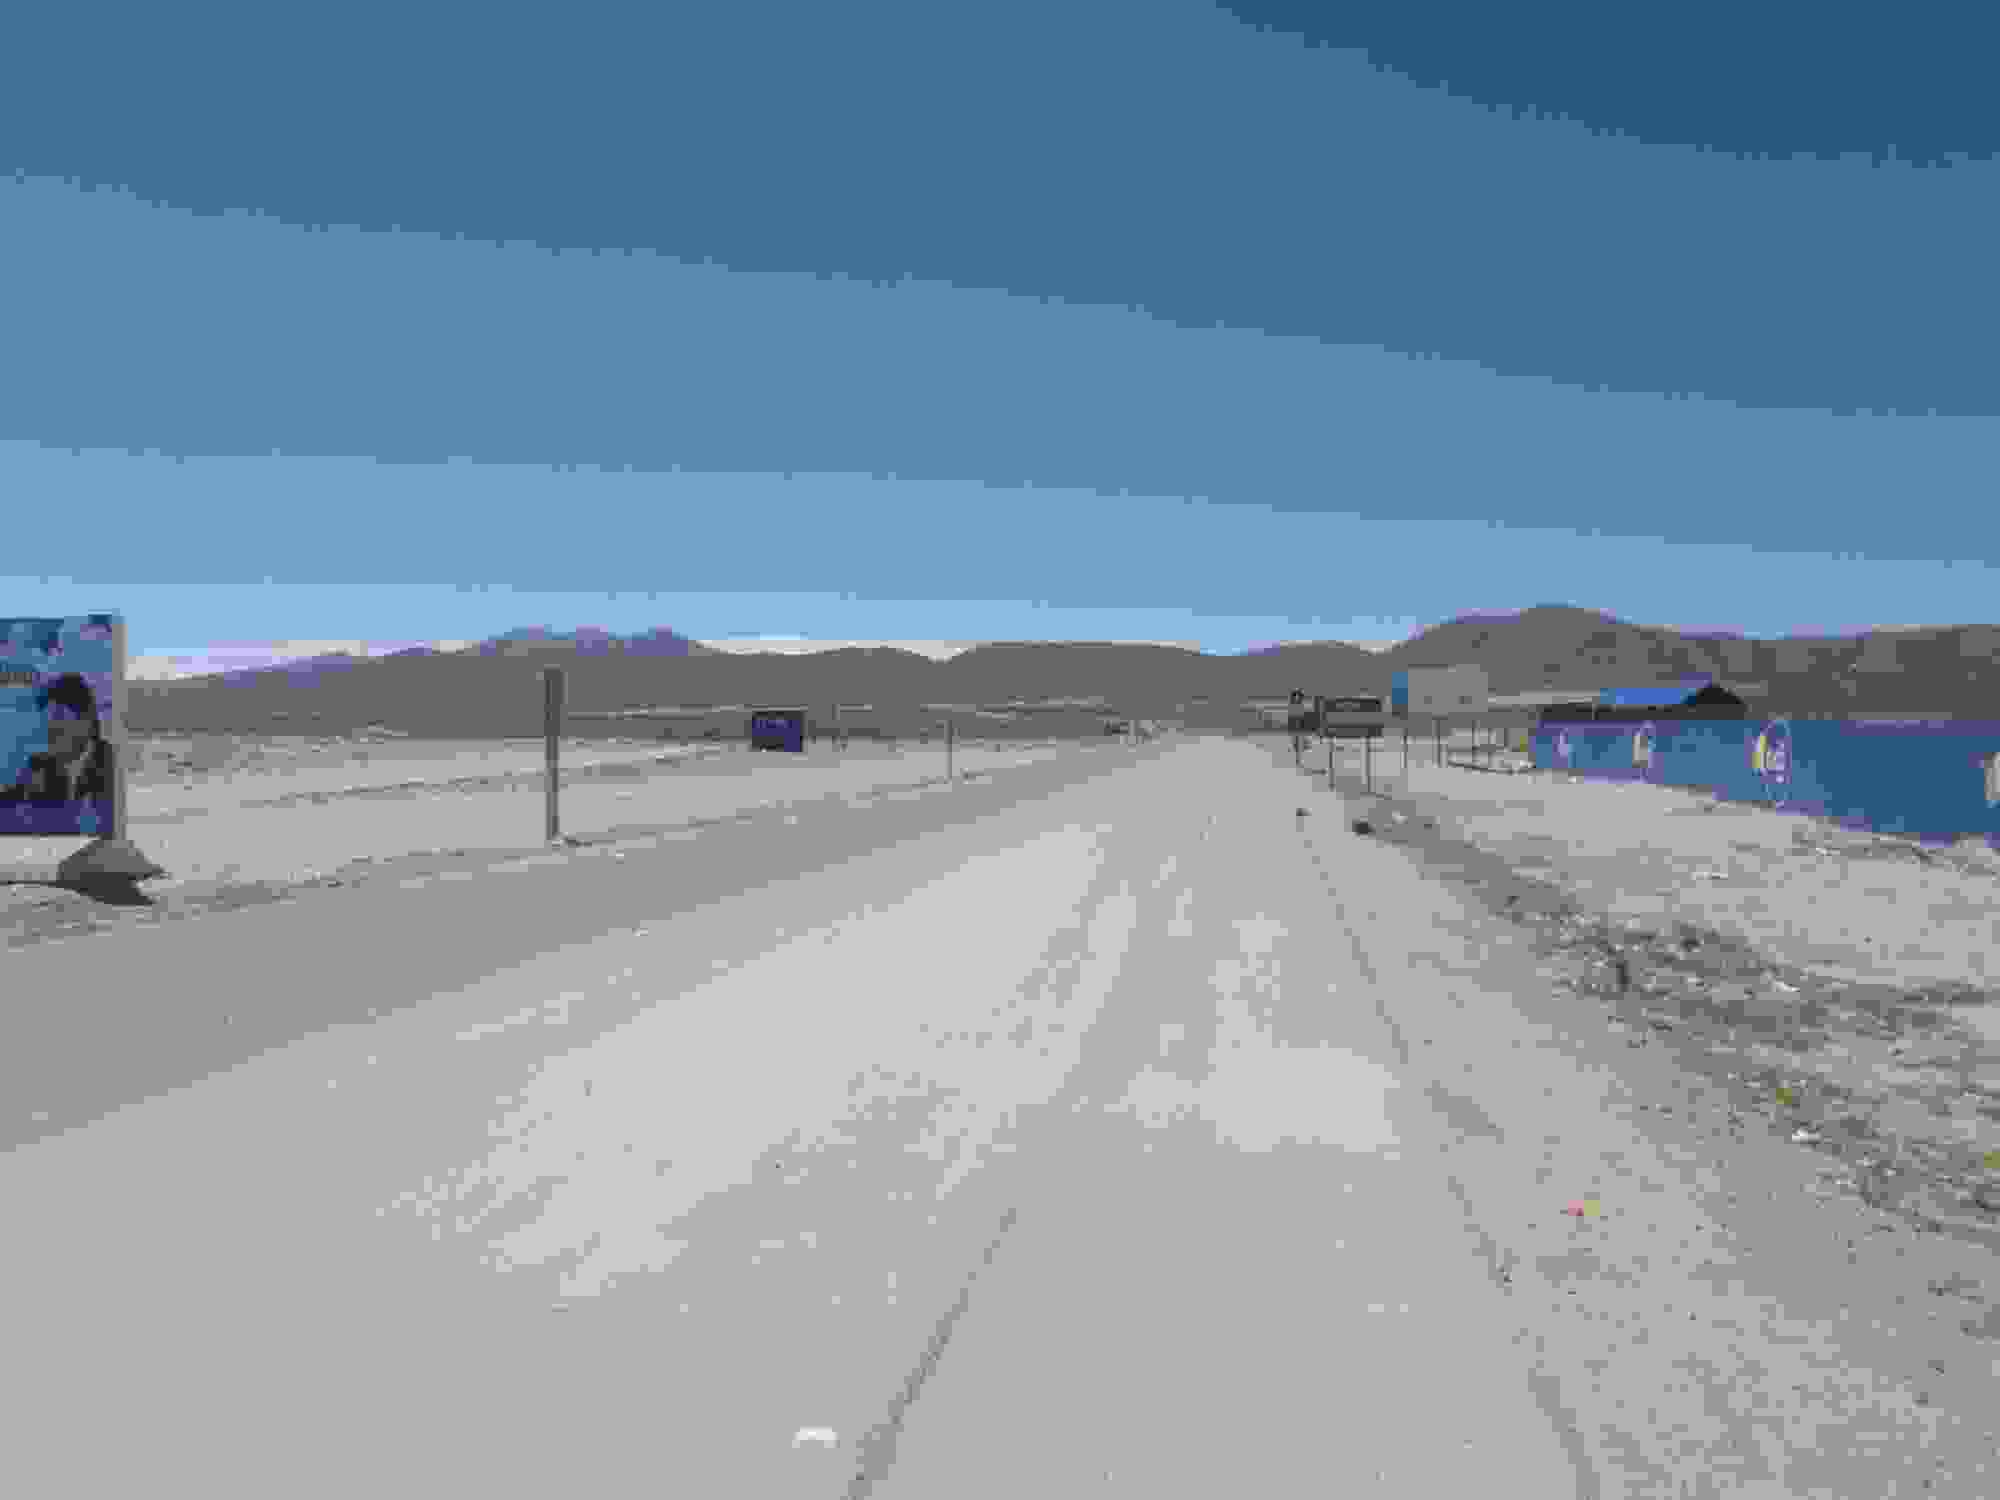
\includegraphics[width=\mywidth]{../wp-content/uploads/2015/04/wpid-wp-1428889869048.jpg} } 
 \newline
 200km avec beaucoup de dénivelé, les paysages sont variés.  \newline
 \newline
\centerline{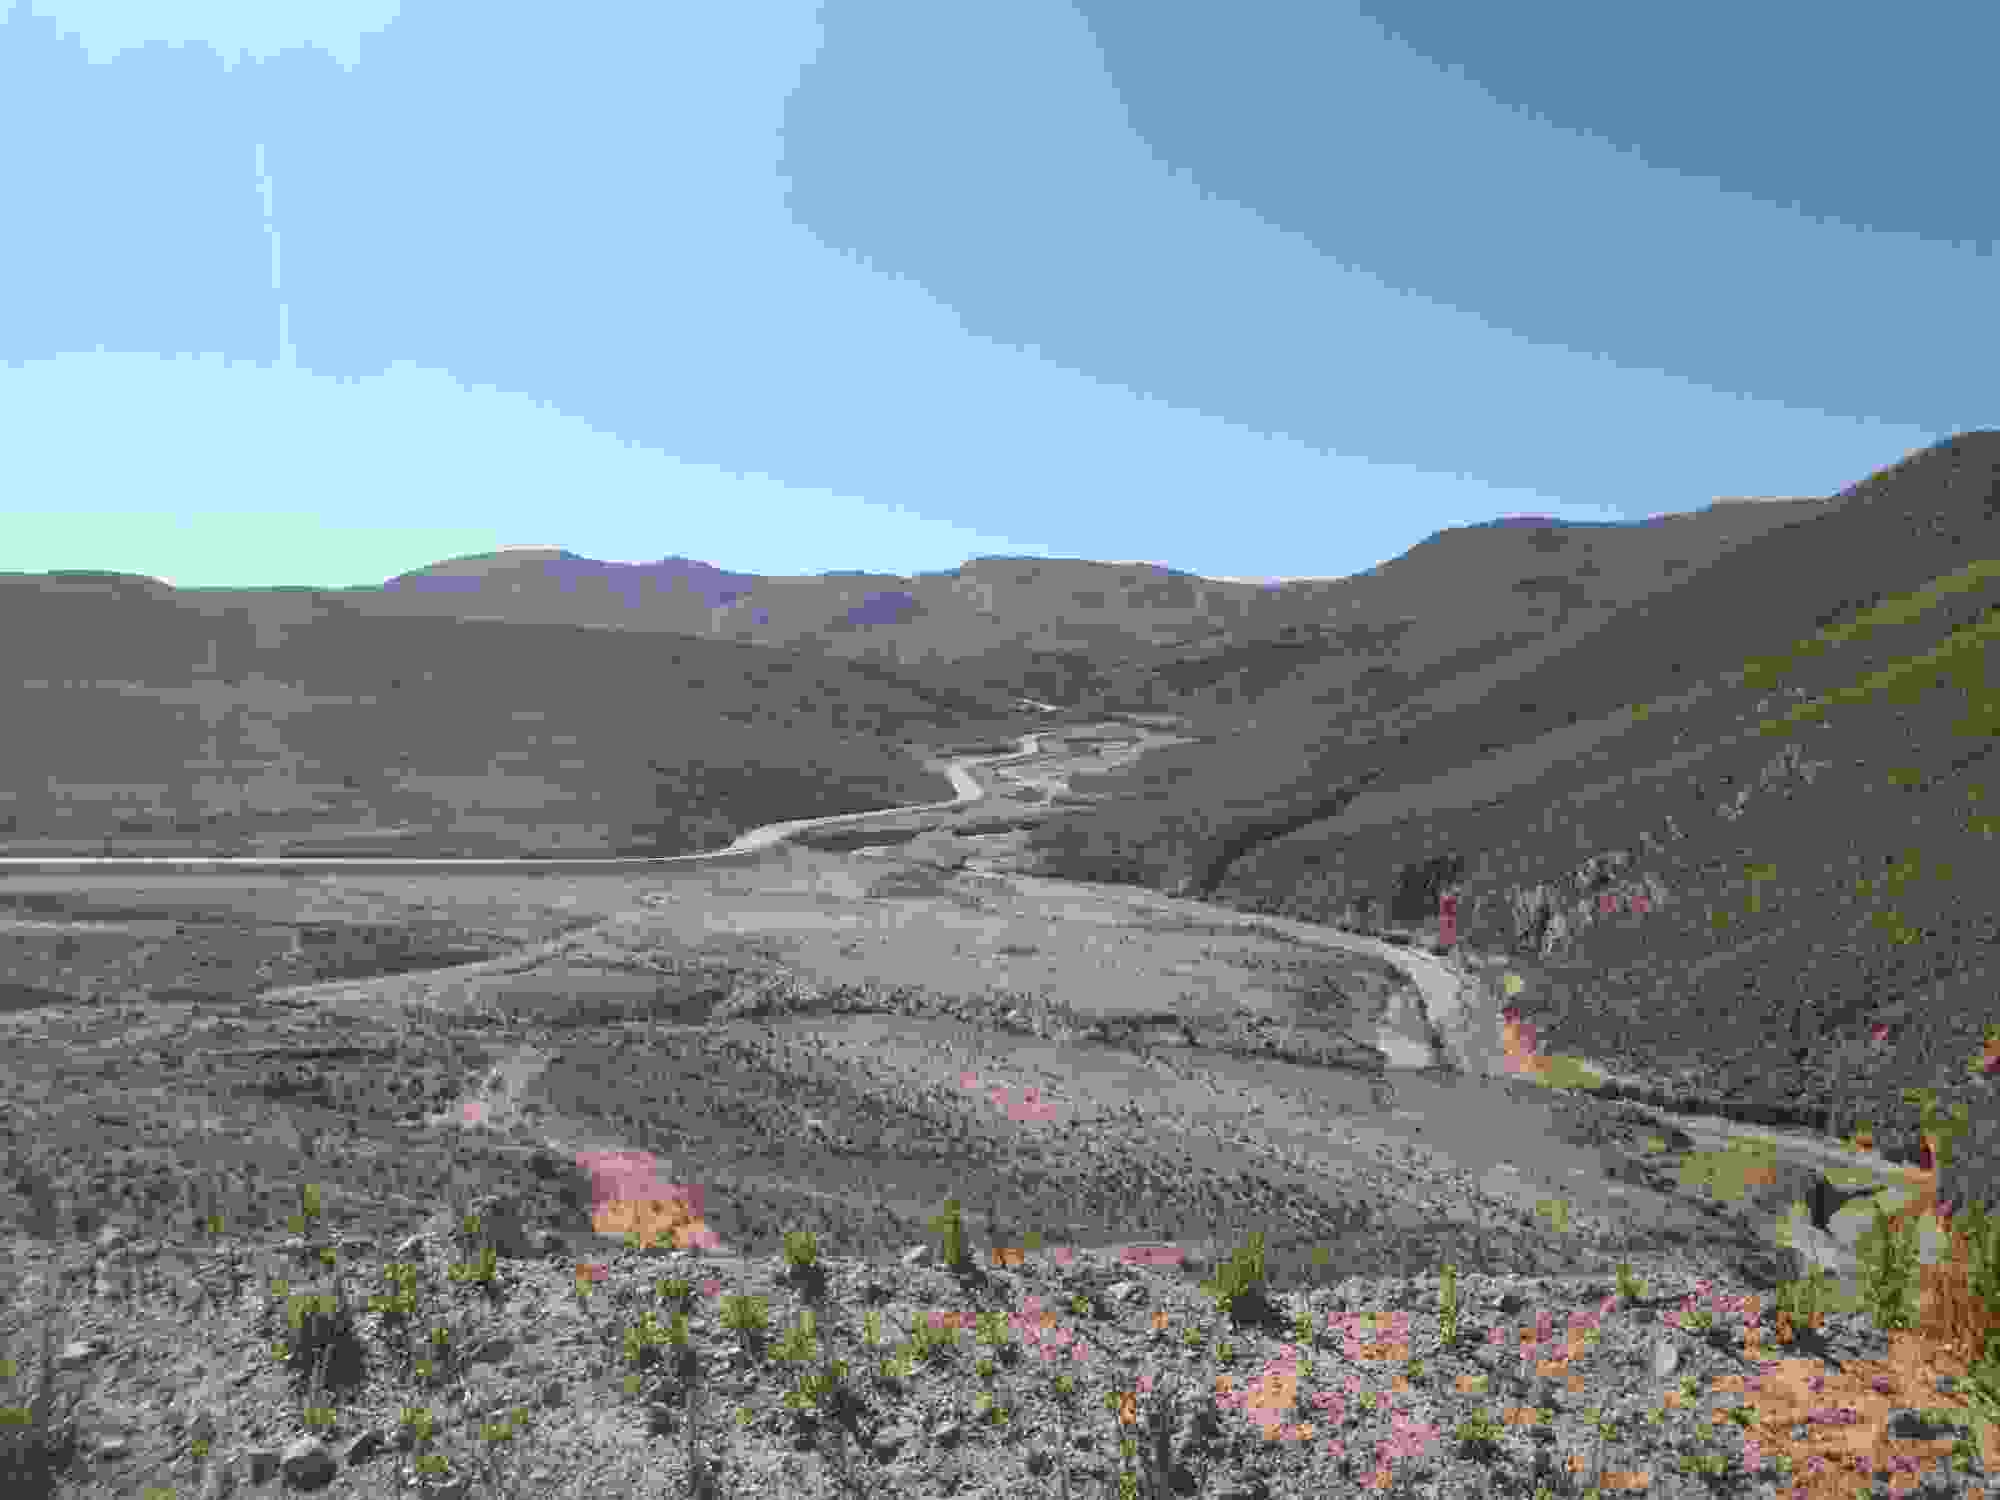
\includegraphics[width=\mywidth]{../wp-content/uploads/2015/04/wpid-wp-1428890082796.jpg} } 
 \newline
 \newline
\centerline{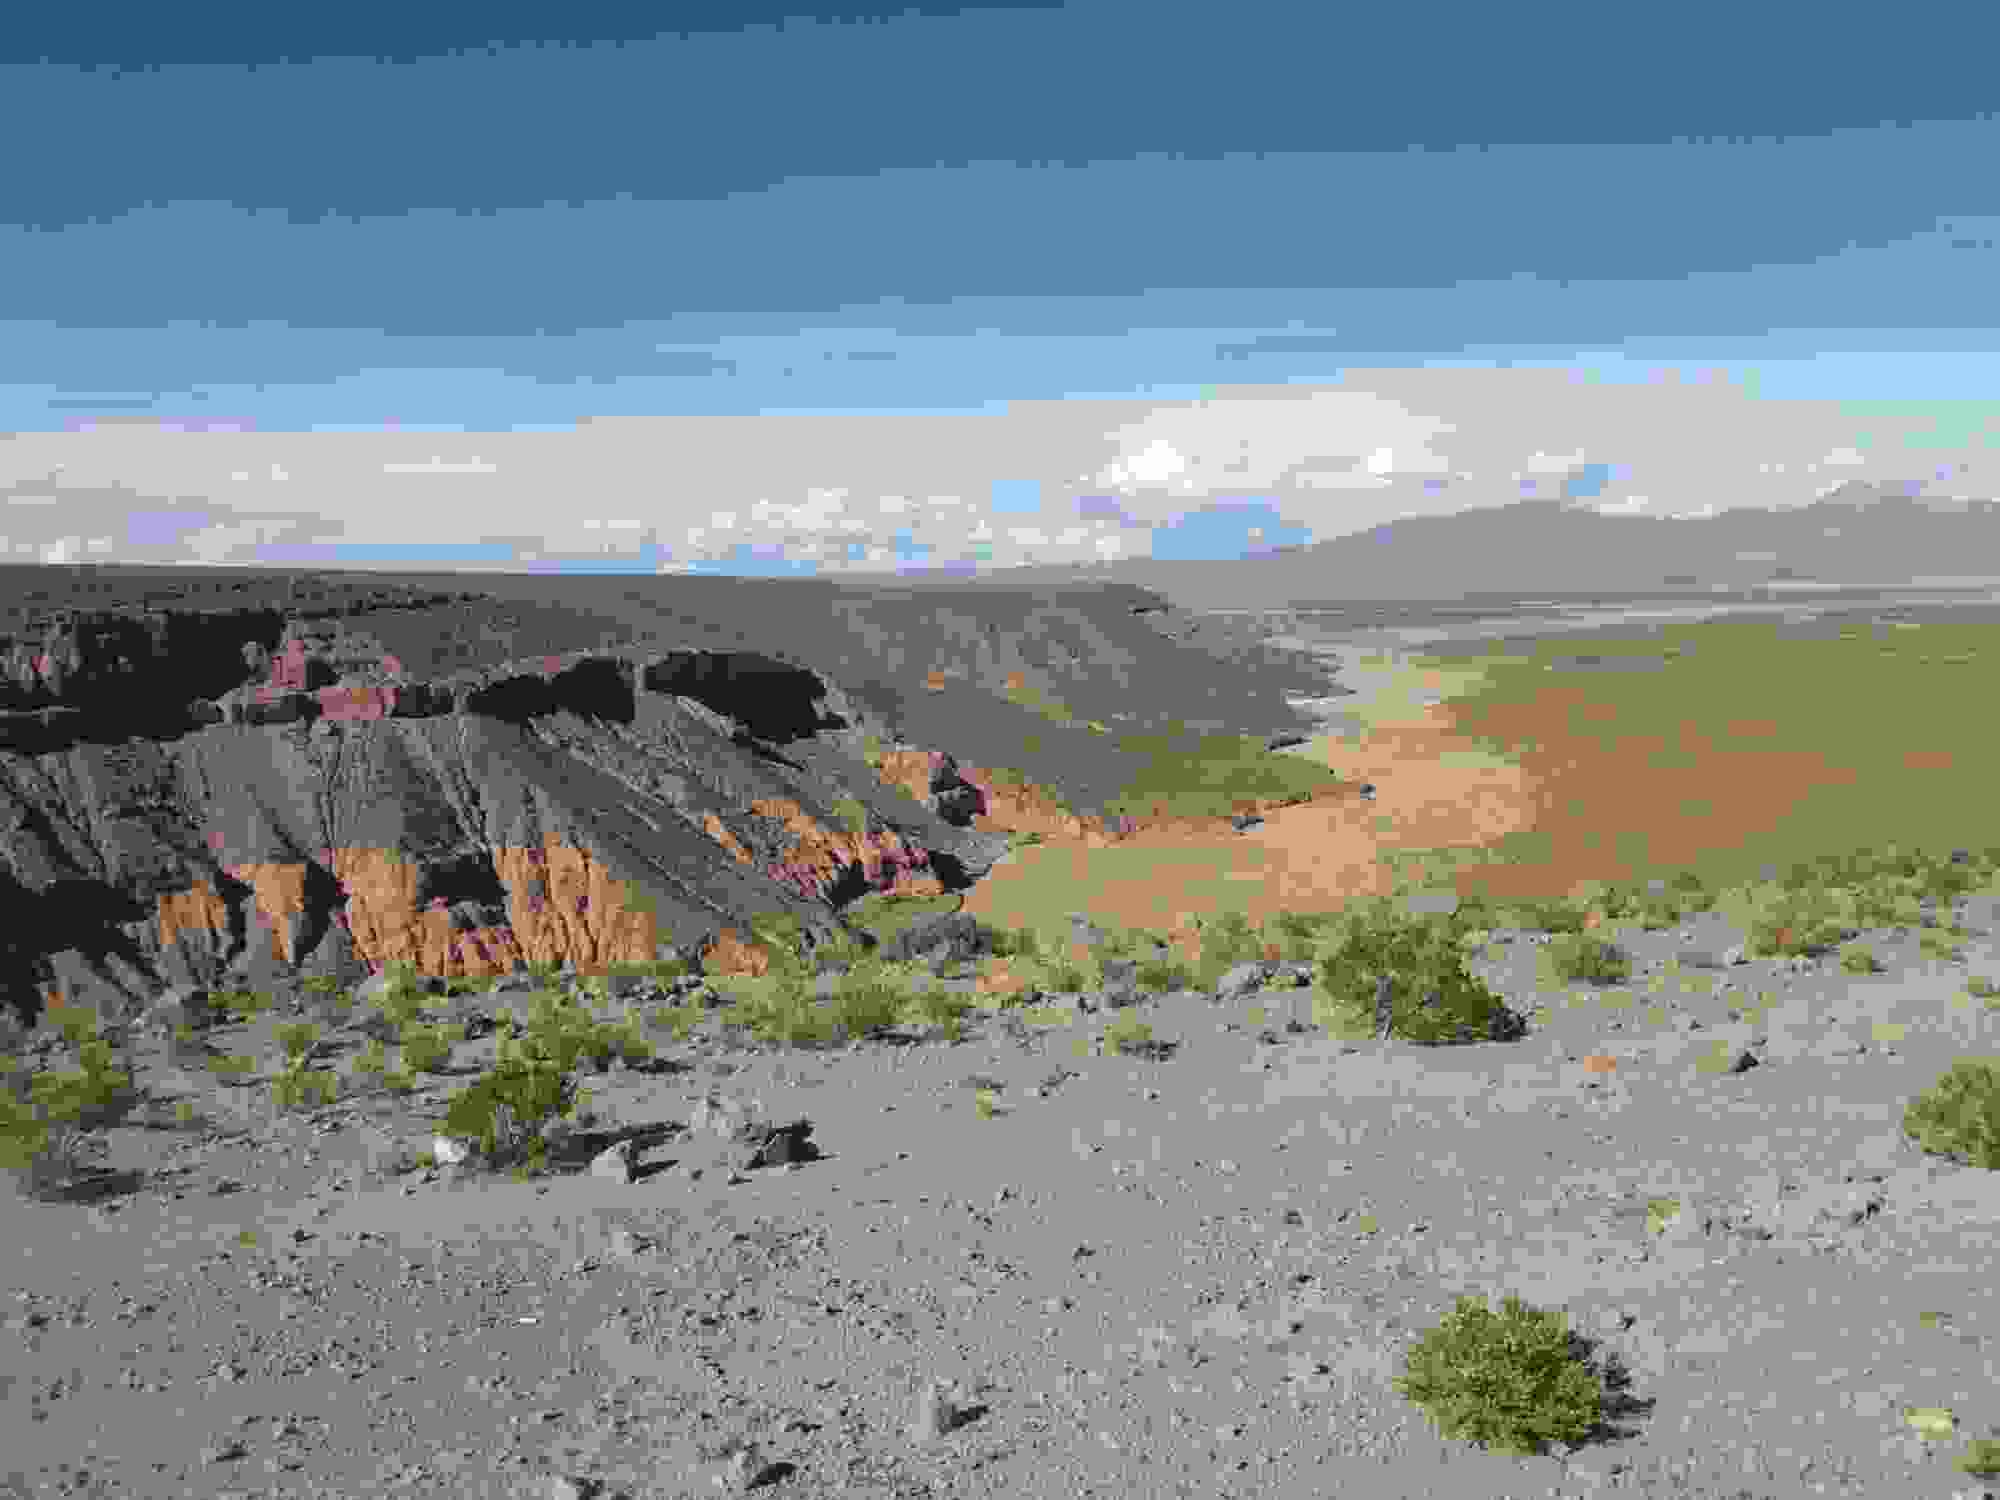
\includegraphics[width=\mywidth]{../wp-content/uploads/2015/04/wpid-wp-1428890125837.jpg} } 
 \newline
 \newline
\centerline{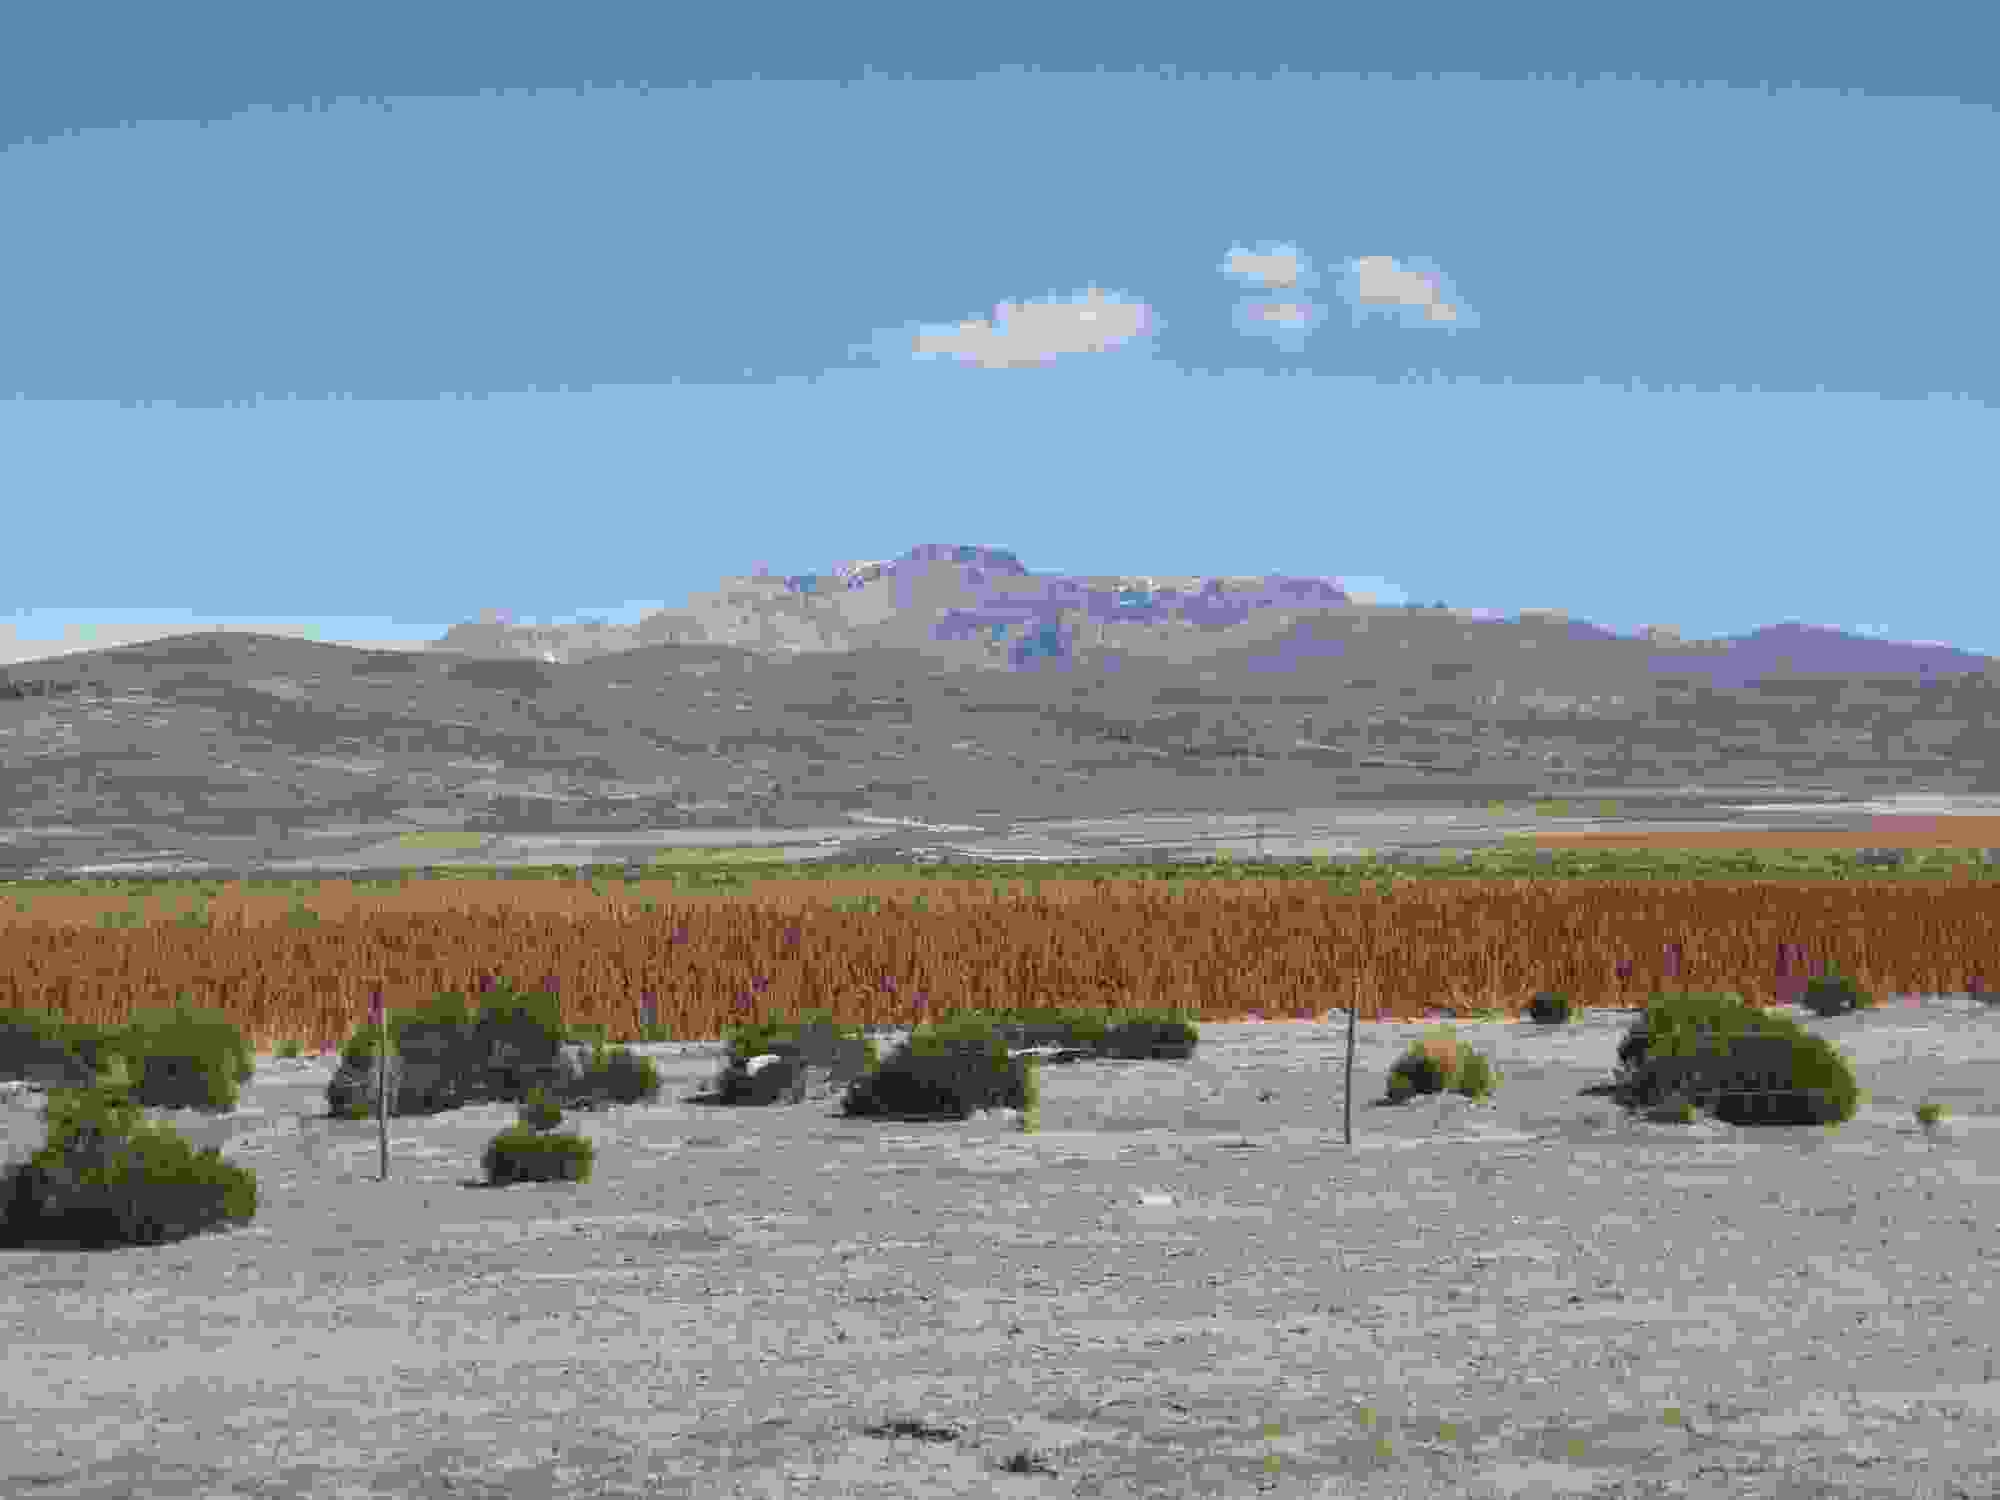
\includegraphics[width=\mywidth]{../wp-content/uploads/2015/04/wpid-wp-1428890169790.jpg} } 
 \newline
 \newline
\centerline{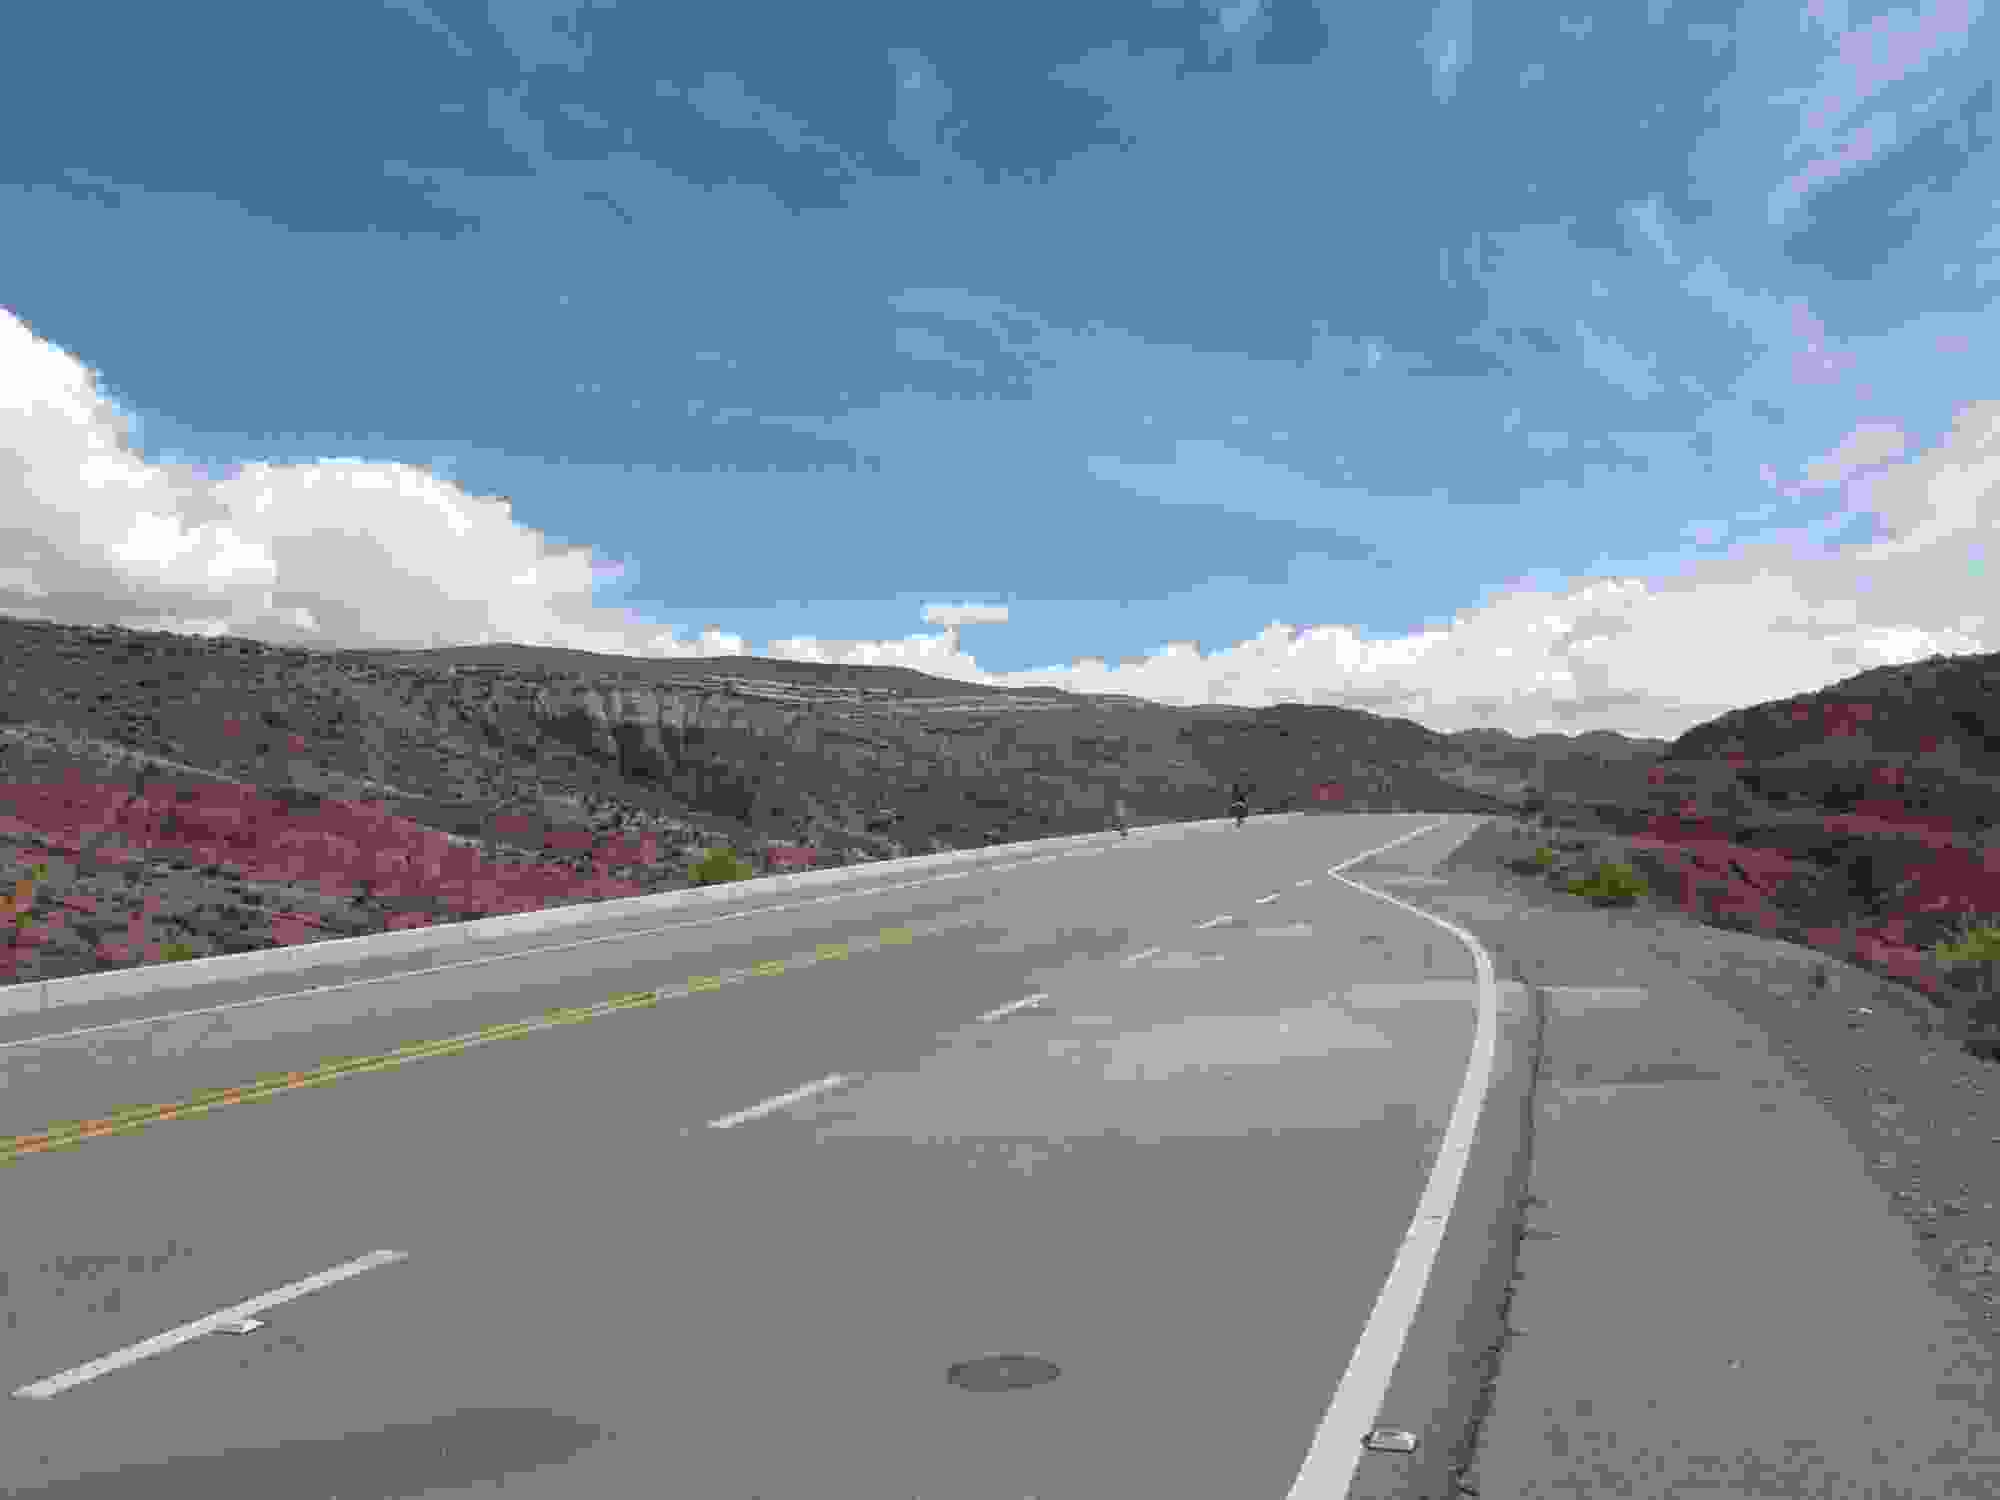
\includegraphics[width=\mywidth]{../wp-content/uploads/2015/04/wpid-wp-1428890252937.jpg} } 
 \newline
 \newline
\centerline{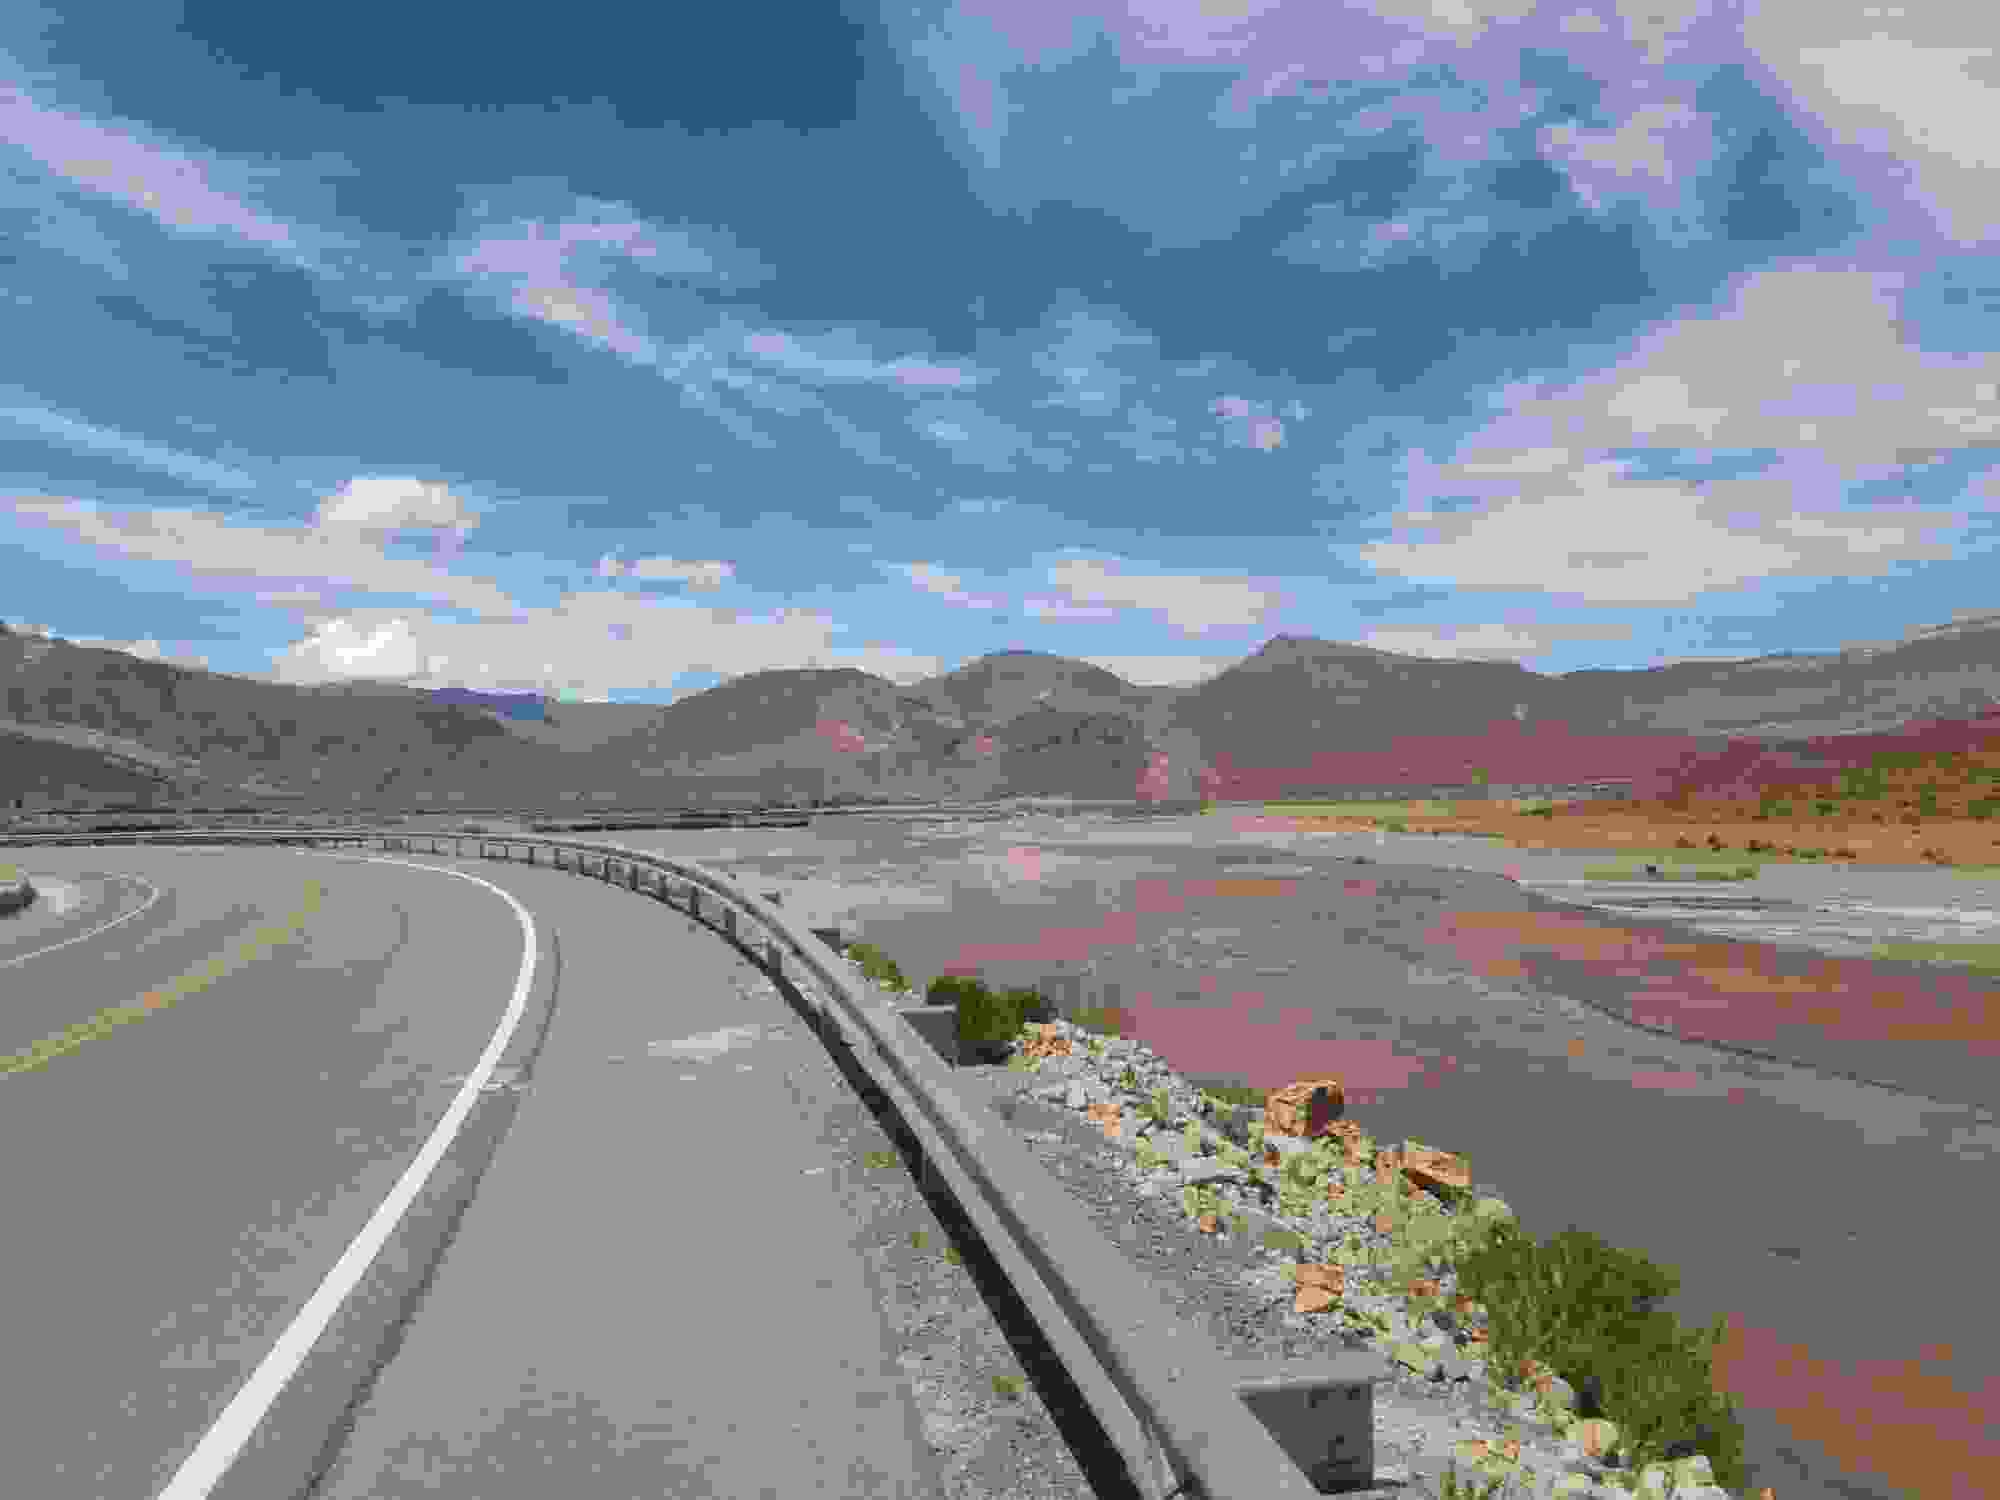
\includegraphics[width=\mywidth]{../wp-content/uploads/2015/04/wpid-wp-1428890285088.jpg} } 
 \newline
 On traverse quelques villages. \newline
 \newline
\centerline{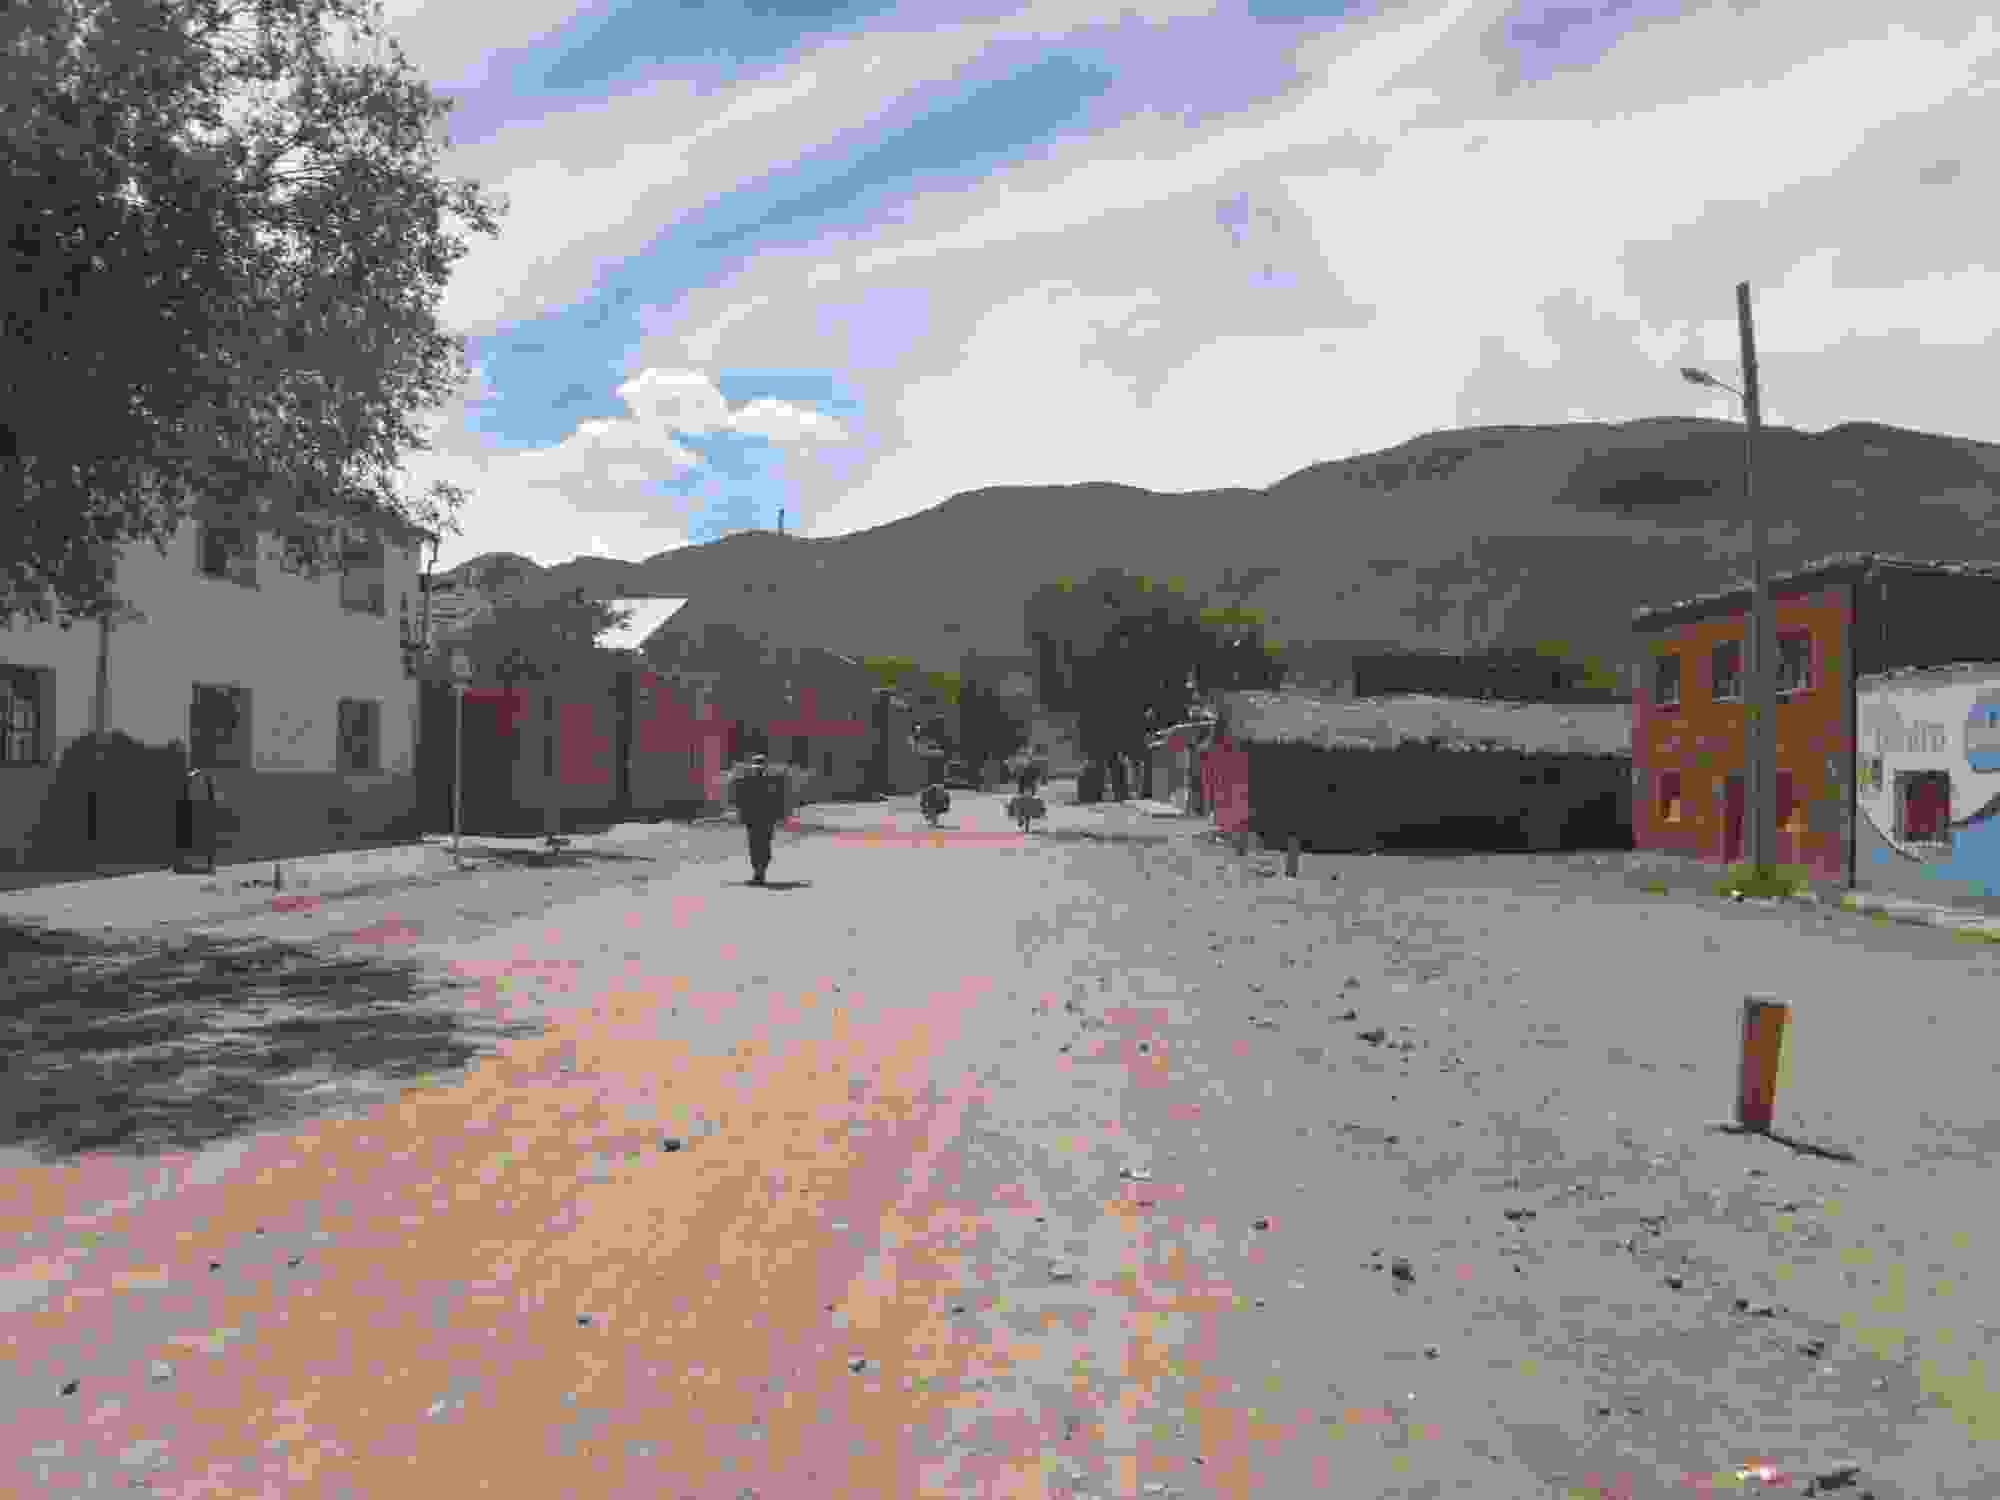
\includegraphics[width=\mywidth]{../wp-content/uploads/2015/04/wpid-wp-1428890373922.jpg} } 
 \newline
 \newline
\centerline{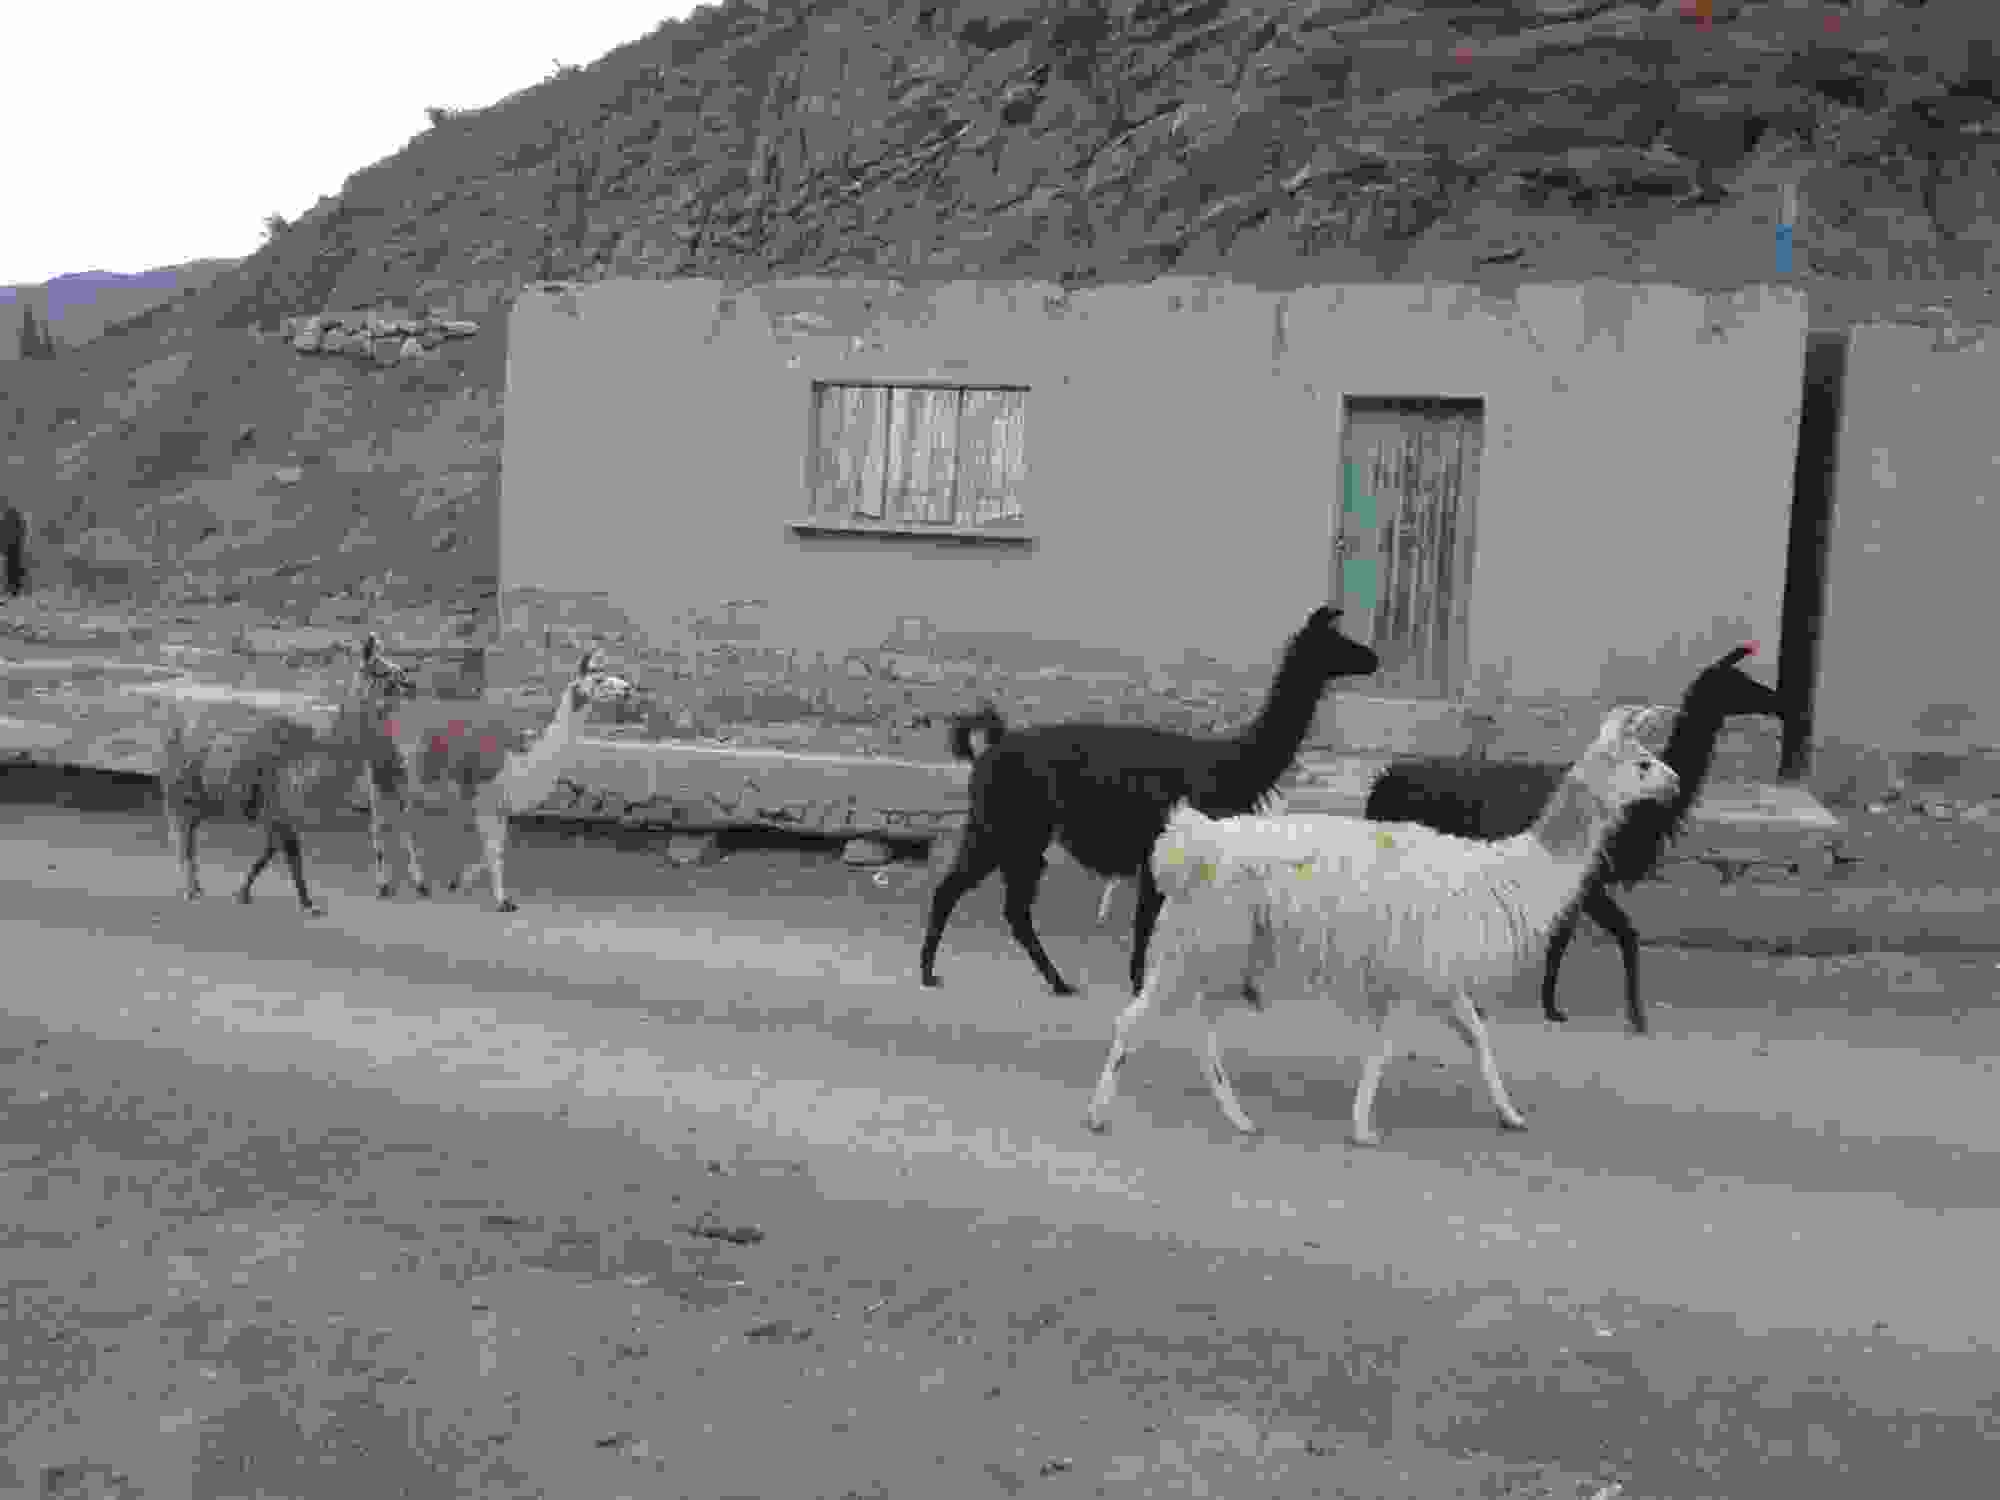
\includegraphics[width=\mywidth]{../wp-content/uploads/2015/04/wpid-wp-1428890480186.jpg} } 
 \newline
 Encore de beaux paysages.  \newline
 \newline
\centerline{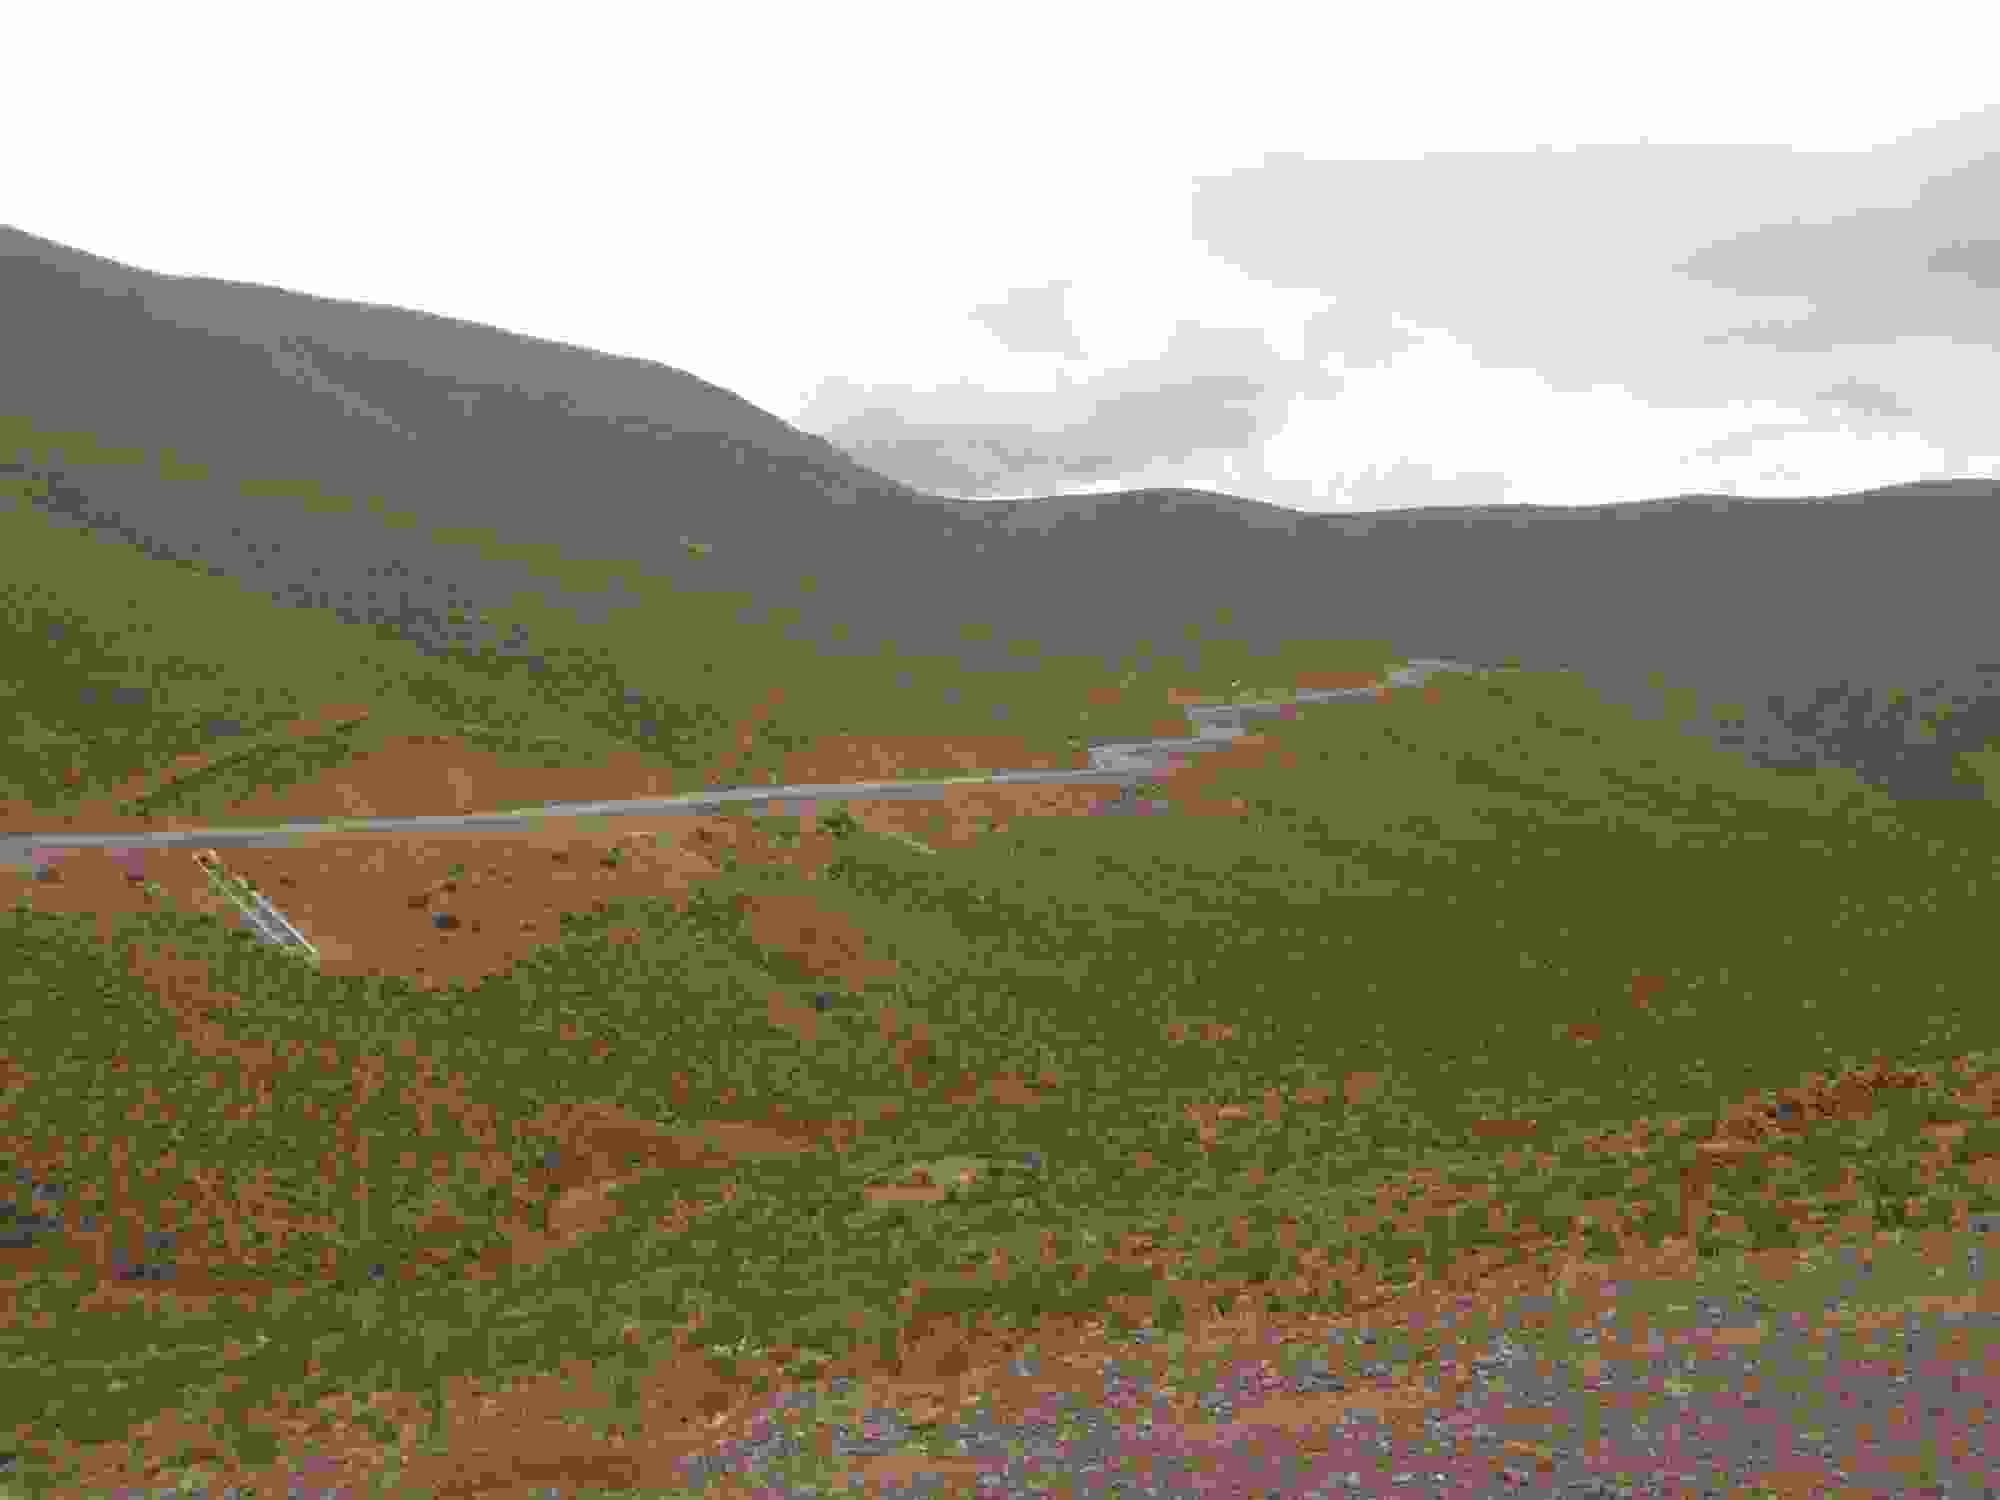
\includegraphics[width=\mywidth]{../wp-content/uploads/2015/04/wpid-wp-1428890534520.jpg} } 
 \newline
 \newline
\centerline{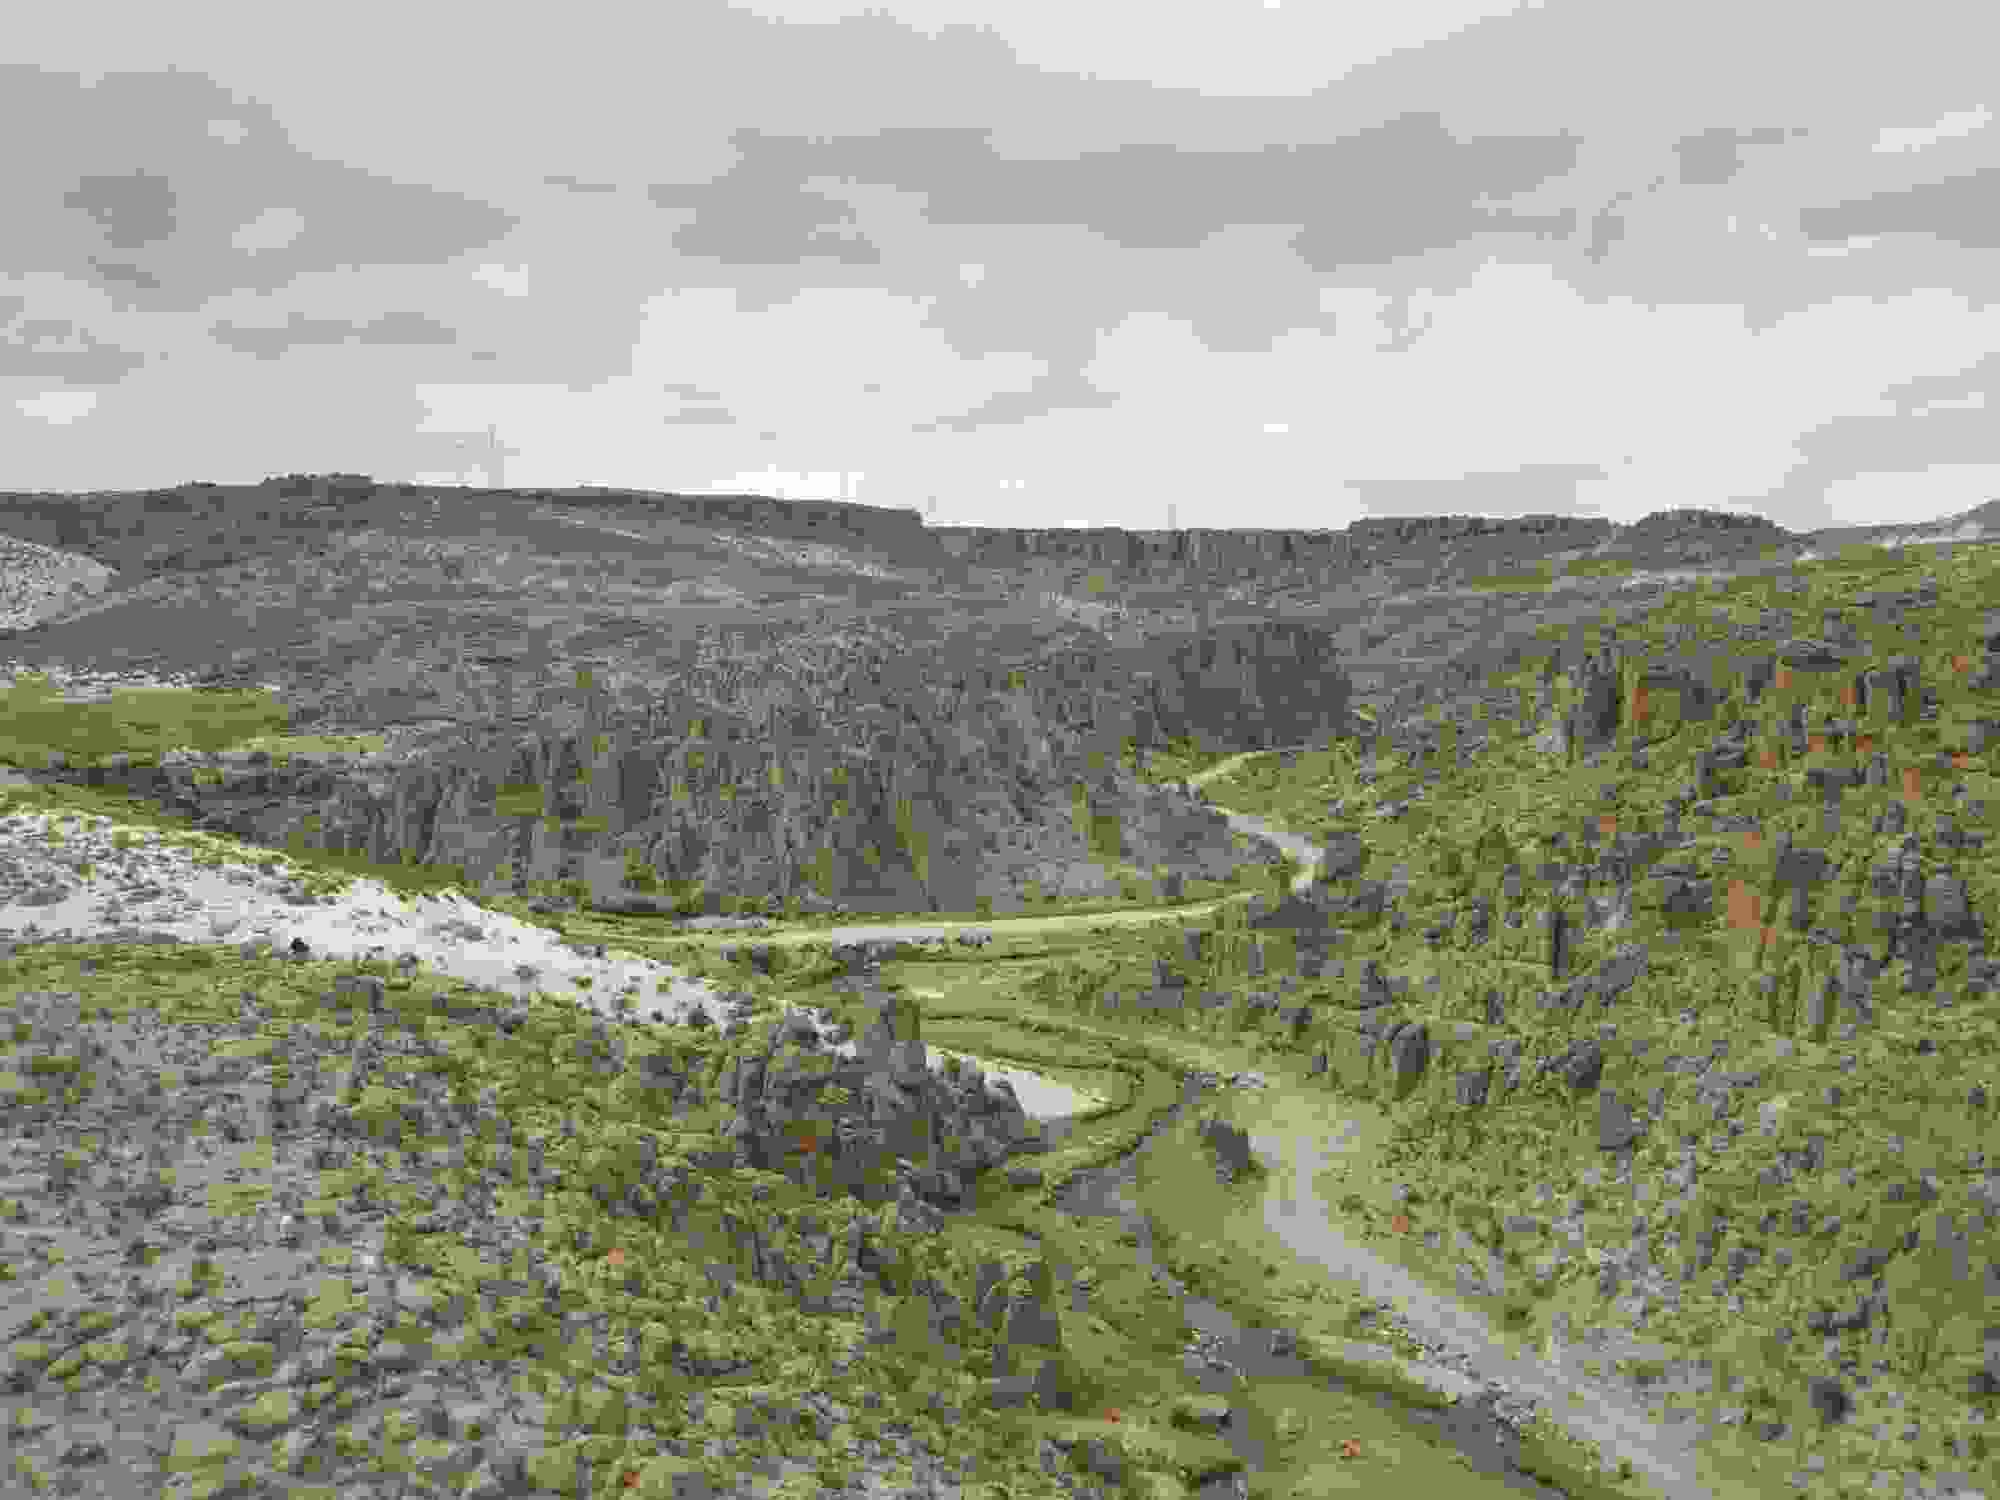
\includegraphics[width=\mywidth]{../wp-content/uploads/2015/04/wpid-wp-1428890635363.jpg} } 
 \newline
 Puis c'est l'arrivée à Potosi \newline
 \newline
\centerline{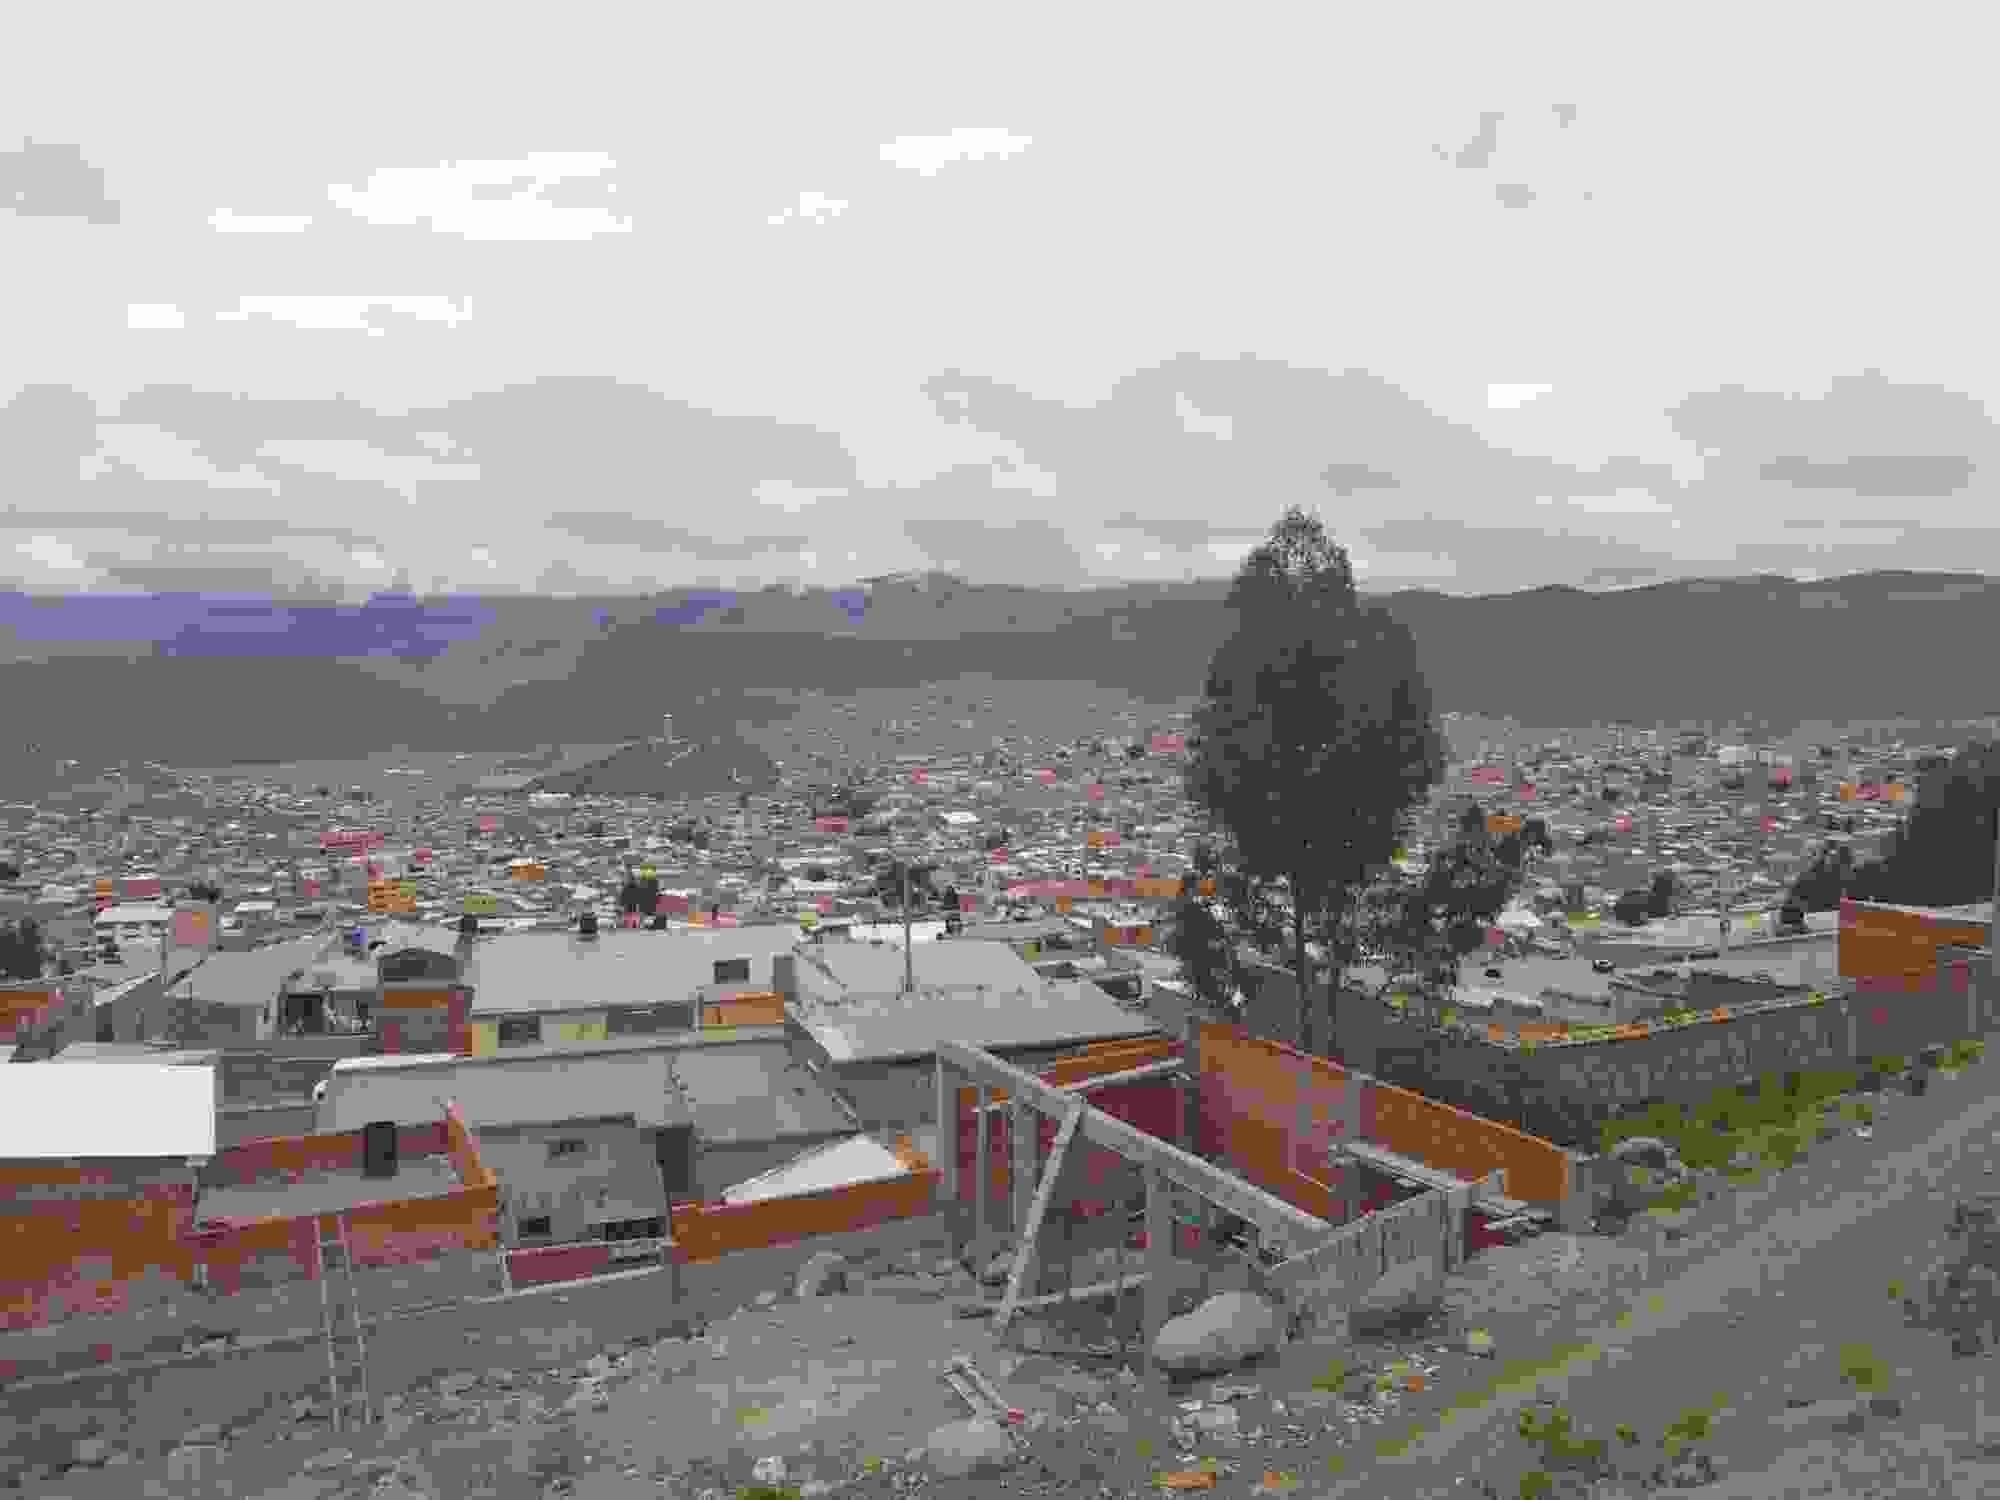
\includegraphics[width=\mywidth]{../wp-content/uploads/2015/04/wpid-wp-1428893483818.jpg} } 
 \newline
 Un lac de couleur bizarre en contrebas de la ville : en fait ce sont les déchets des usines de traitement des minerais. \newline
 \newline
\centerline{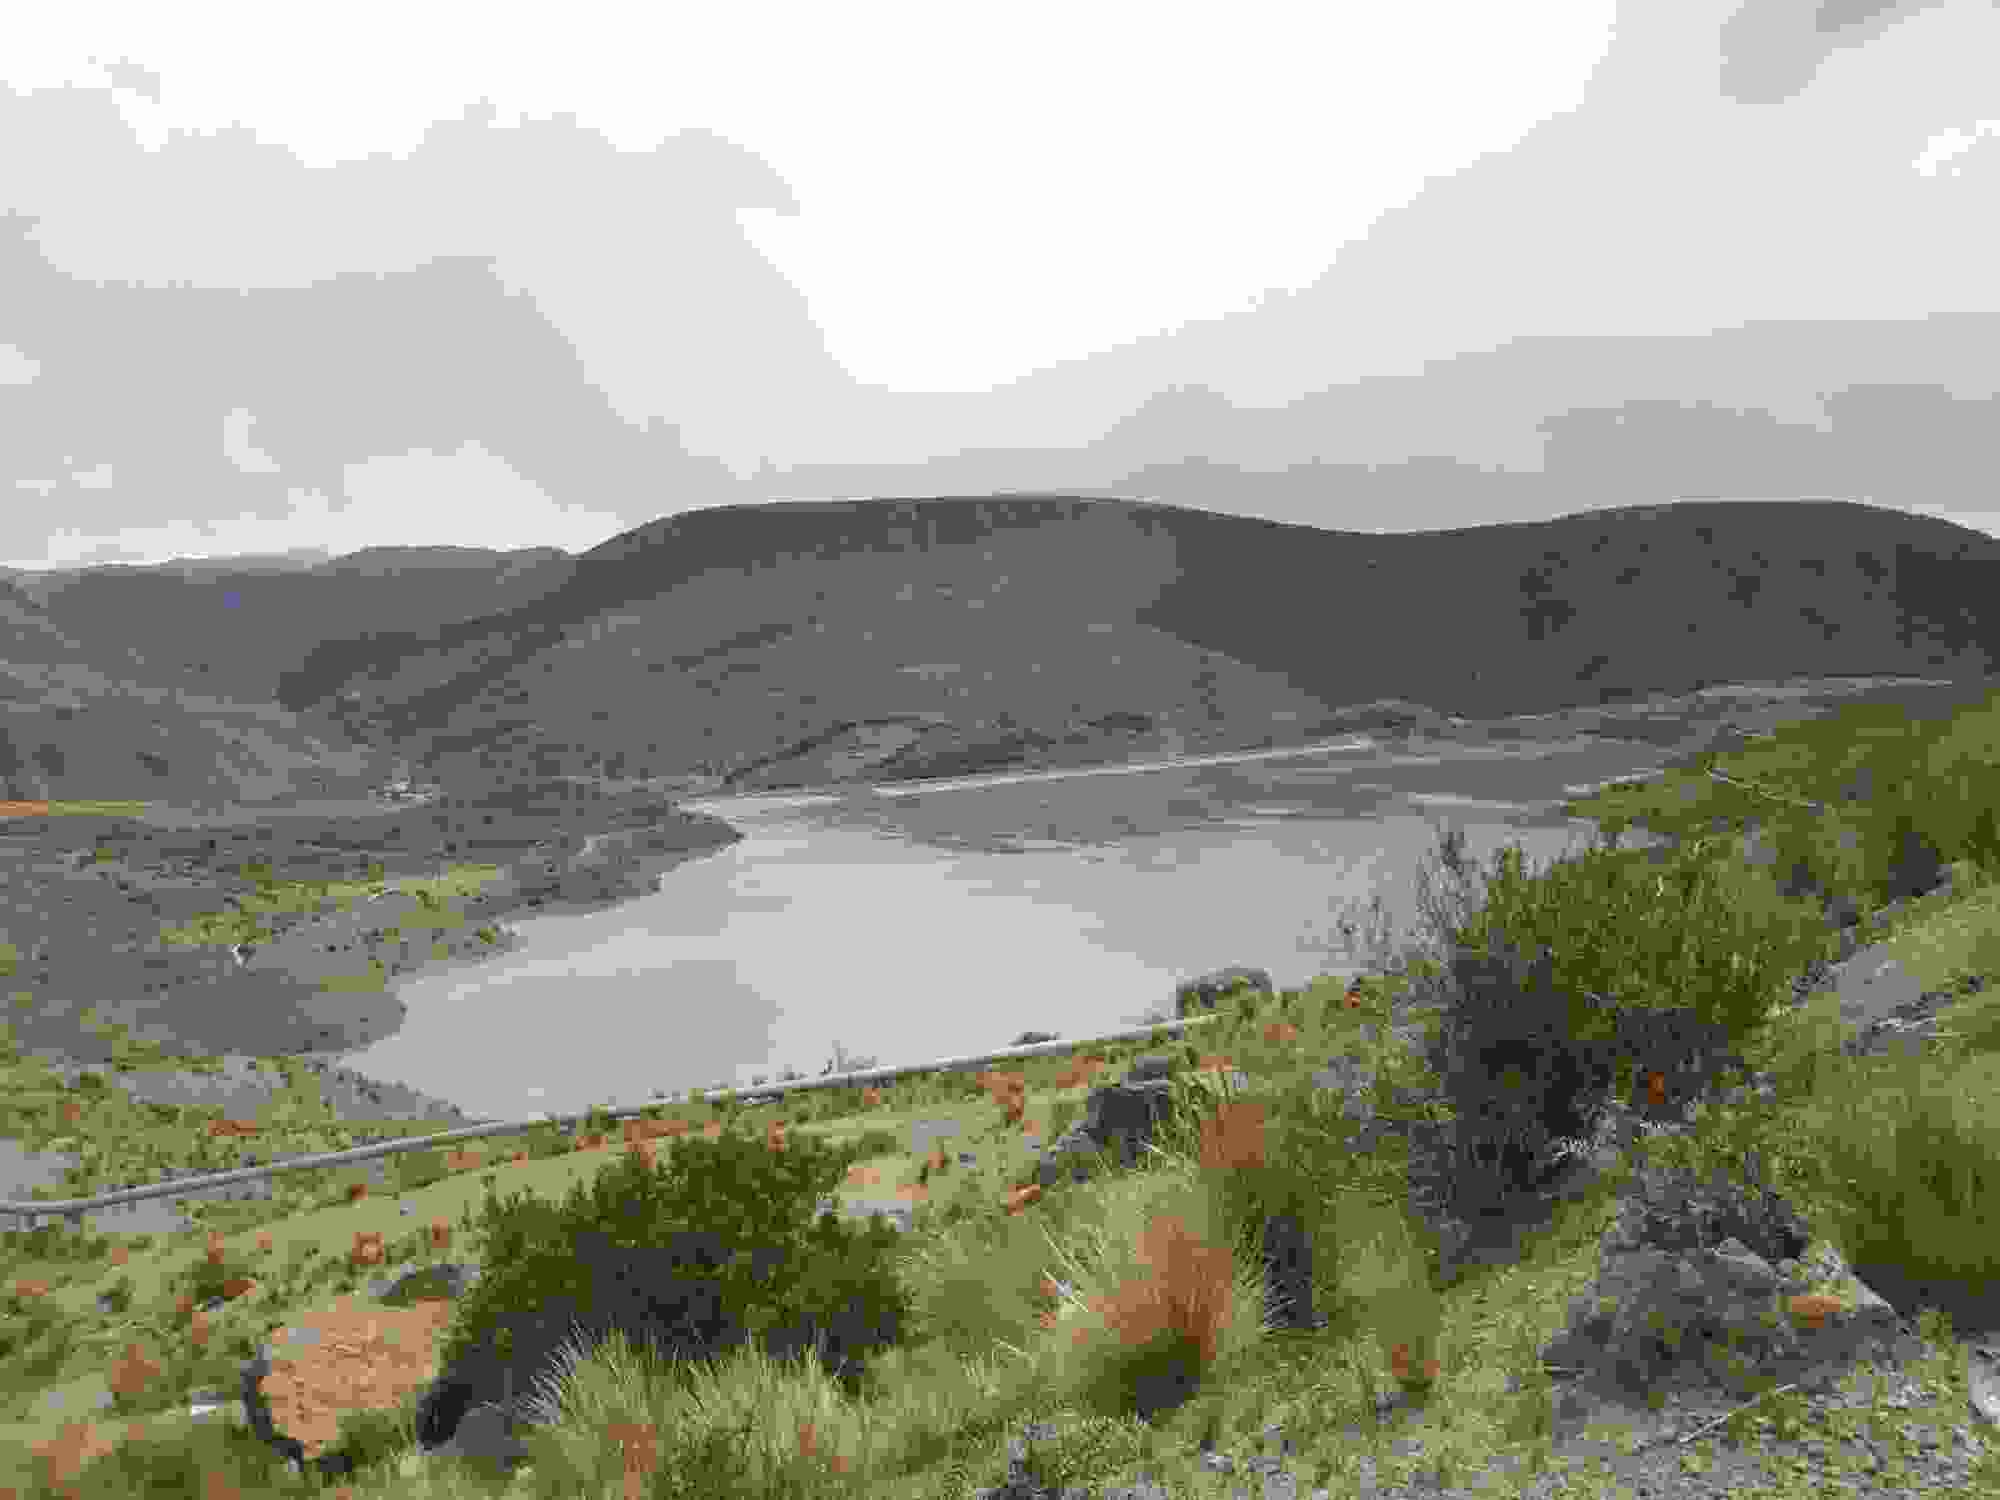
\includegraphics[width=\mywidth]{../wp-content/uploads/2015/04/wpid-wp-1428891087219.jpg} } 
 \newline
 Le centre de Potosi, des petites rues animées et polluées.  \newline
 \newline
\centerline{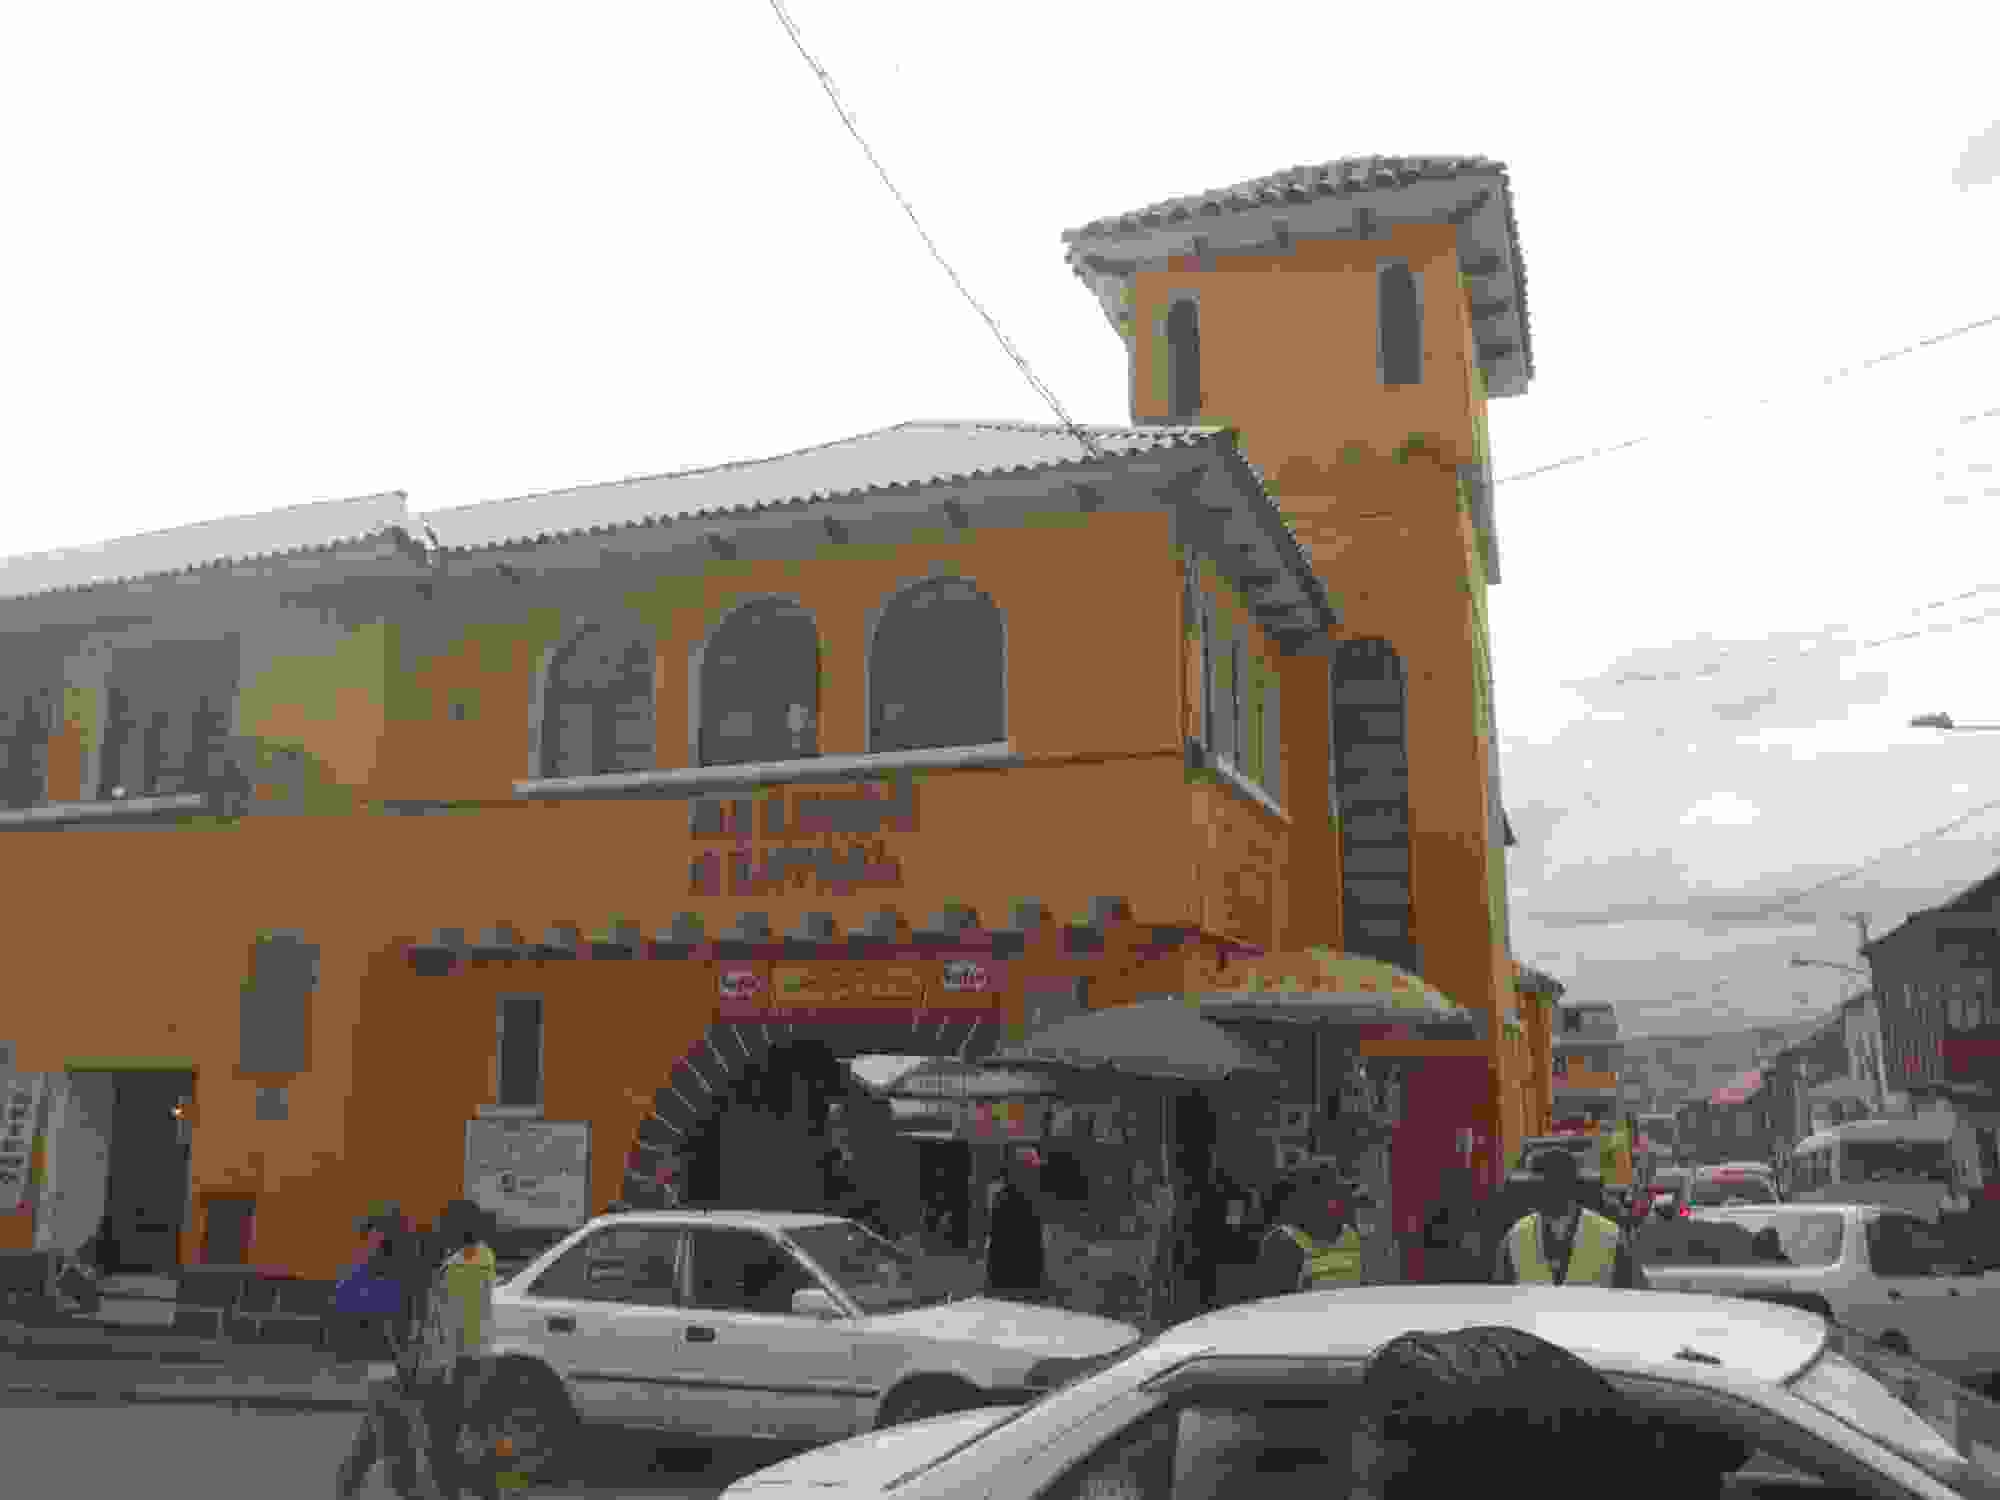
\includegraphics[width=\mywidth]{../wp-content/uploads/2015/04/wpid-wp-1428891137998.jpg} } 
 \newline
 \newline
\centerline{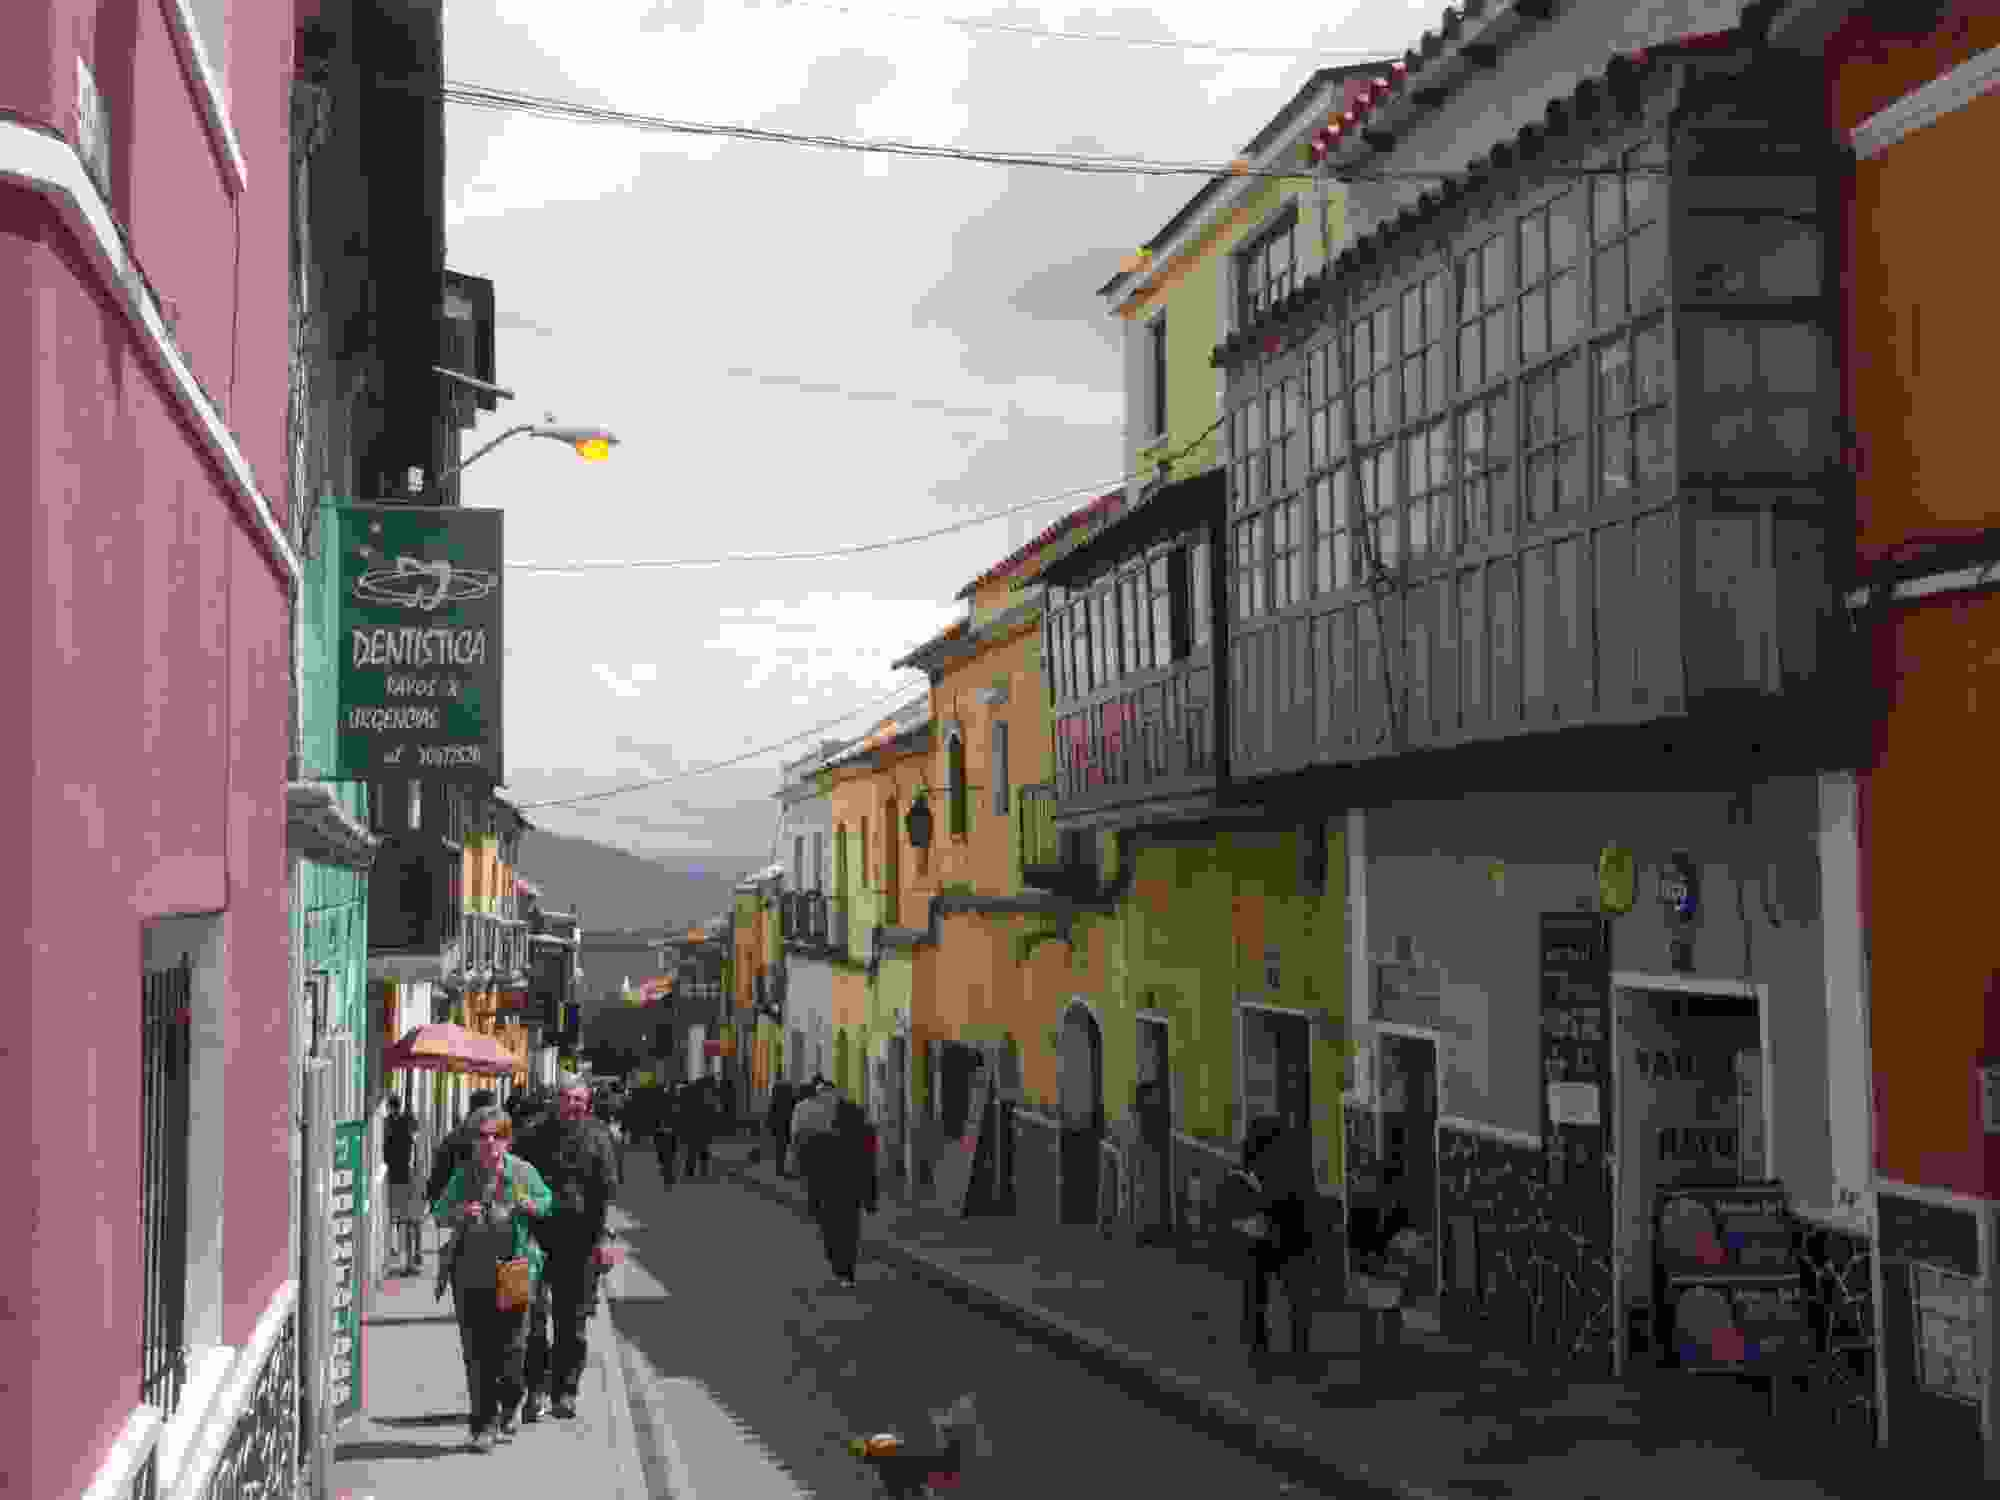
\includegraphics[width=\mywidth]{../wp-content/uploads/2015/04/wpid-wp-1428891177251.jpg} } 
 \newline
 \newline
\centerline{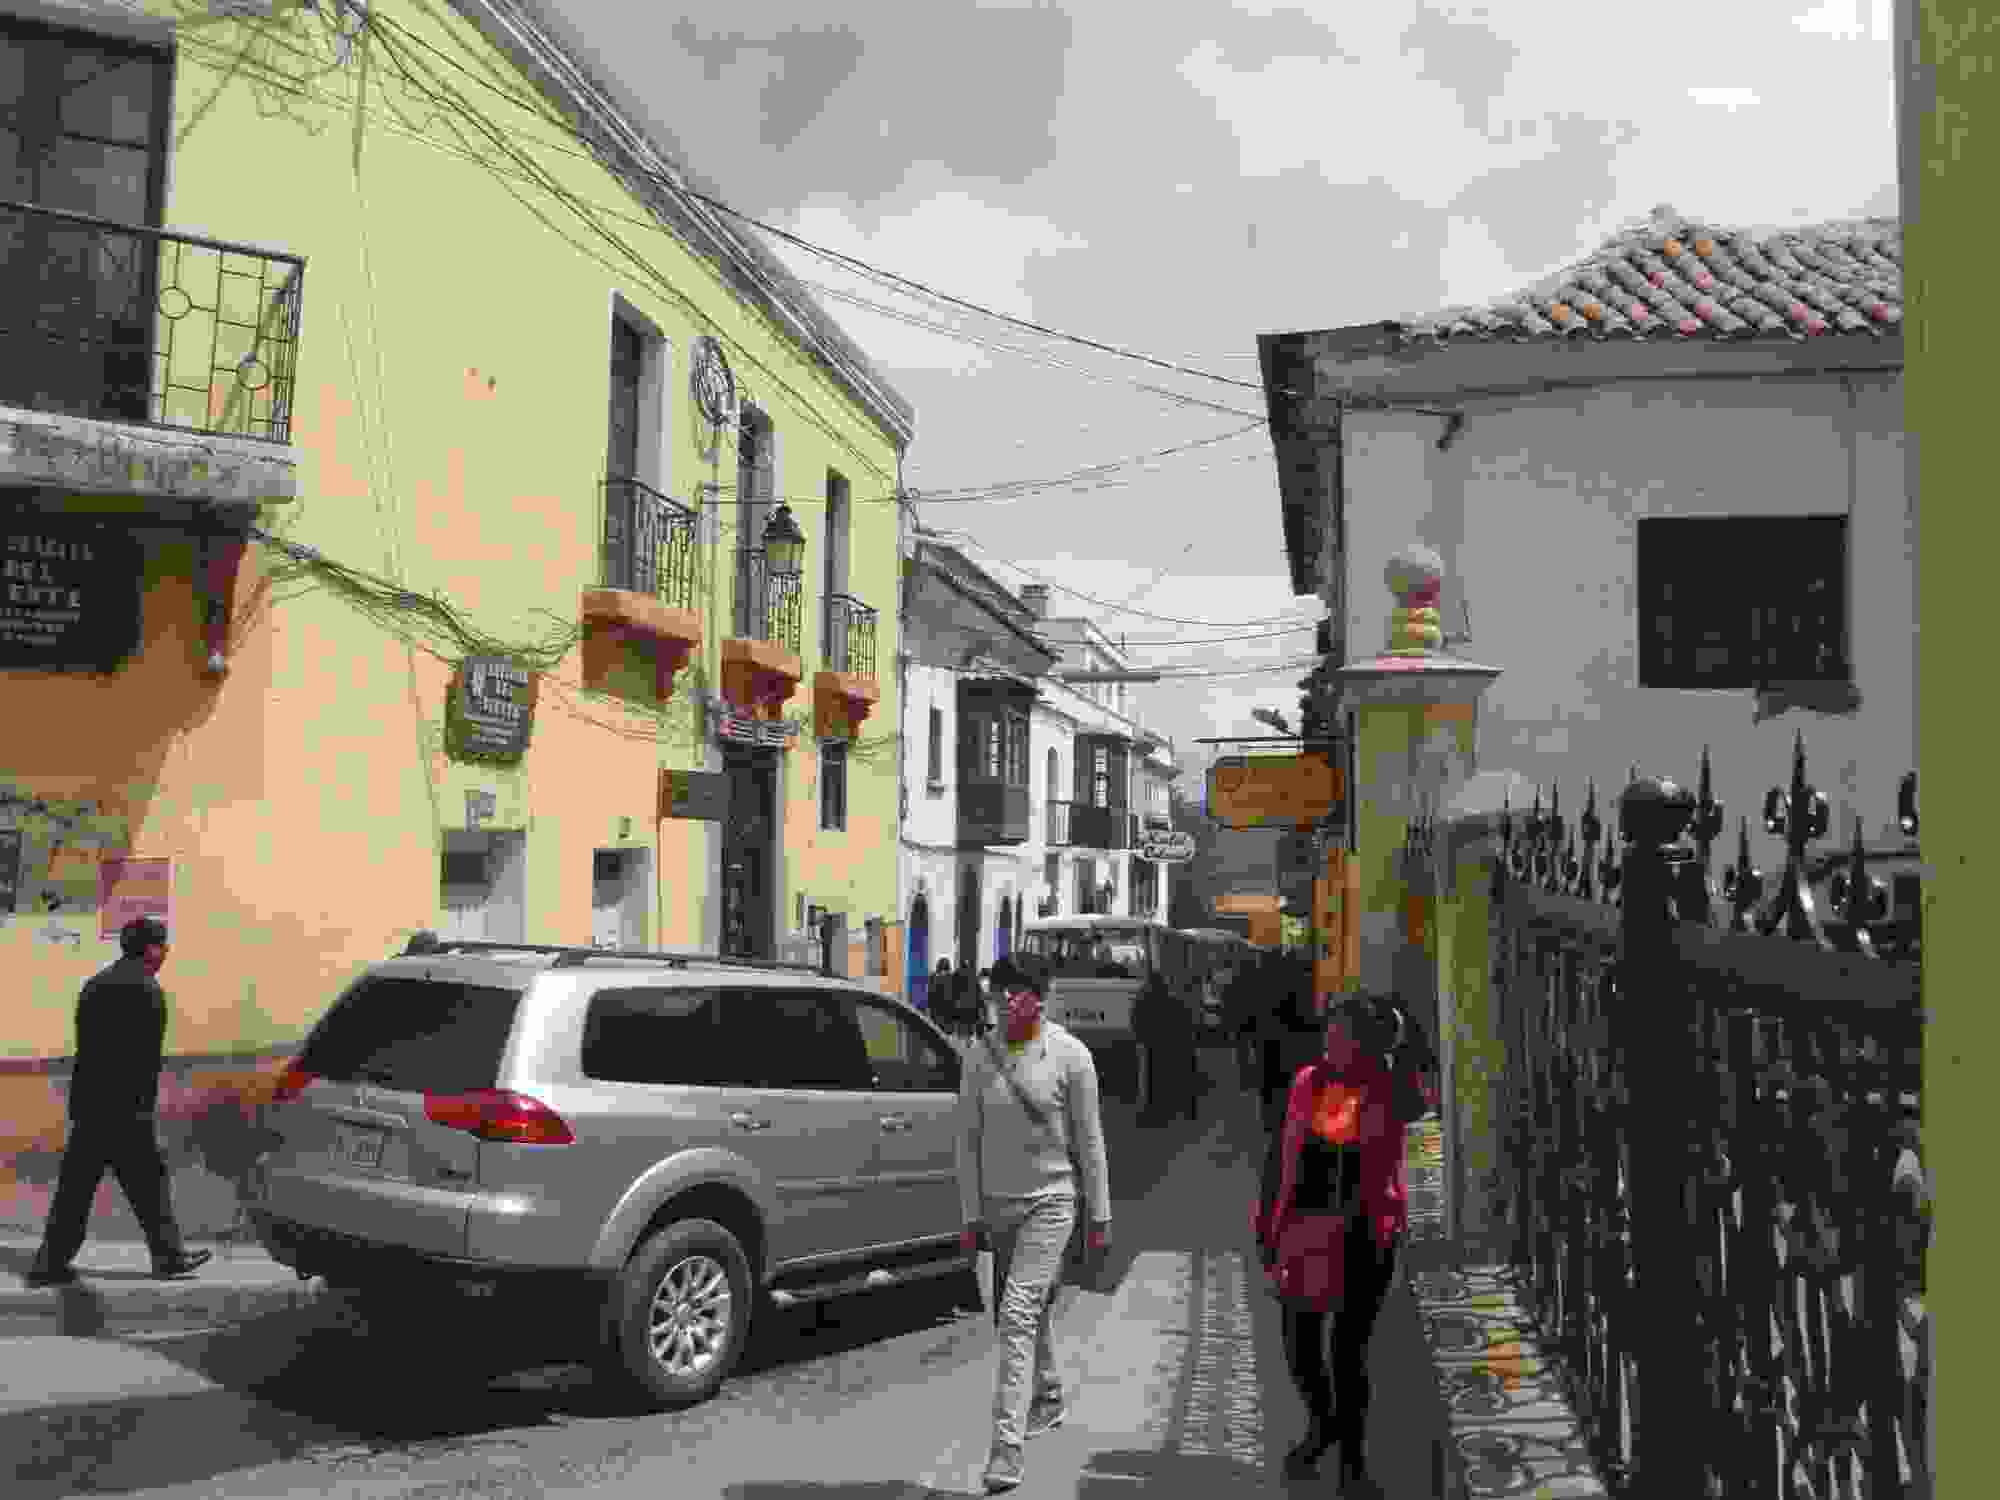
\includegraphics[width=\mywidth]{../wp-content/uploads/2015/04/wpid-wp-1428891217403.jpg} } 
 \newline
 La cathédrale \newline
 \newline
\centerline{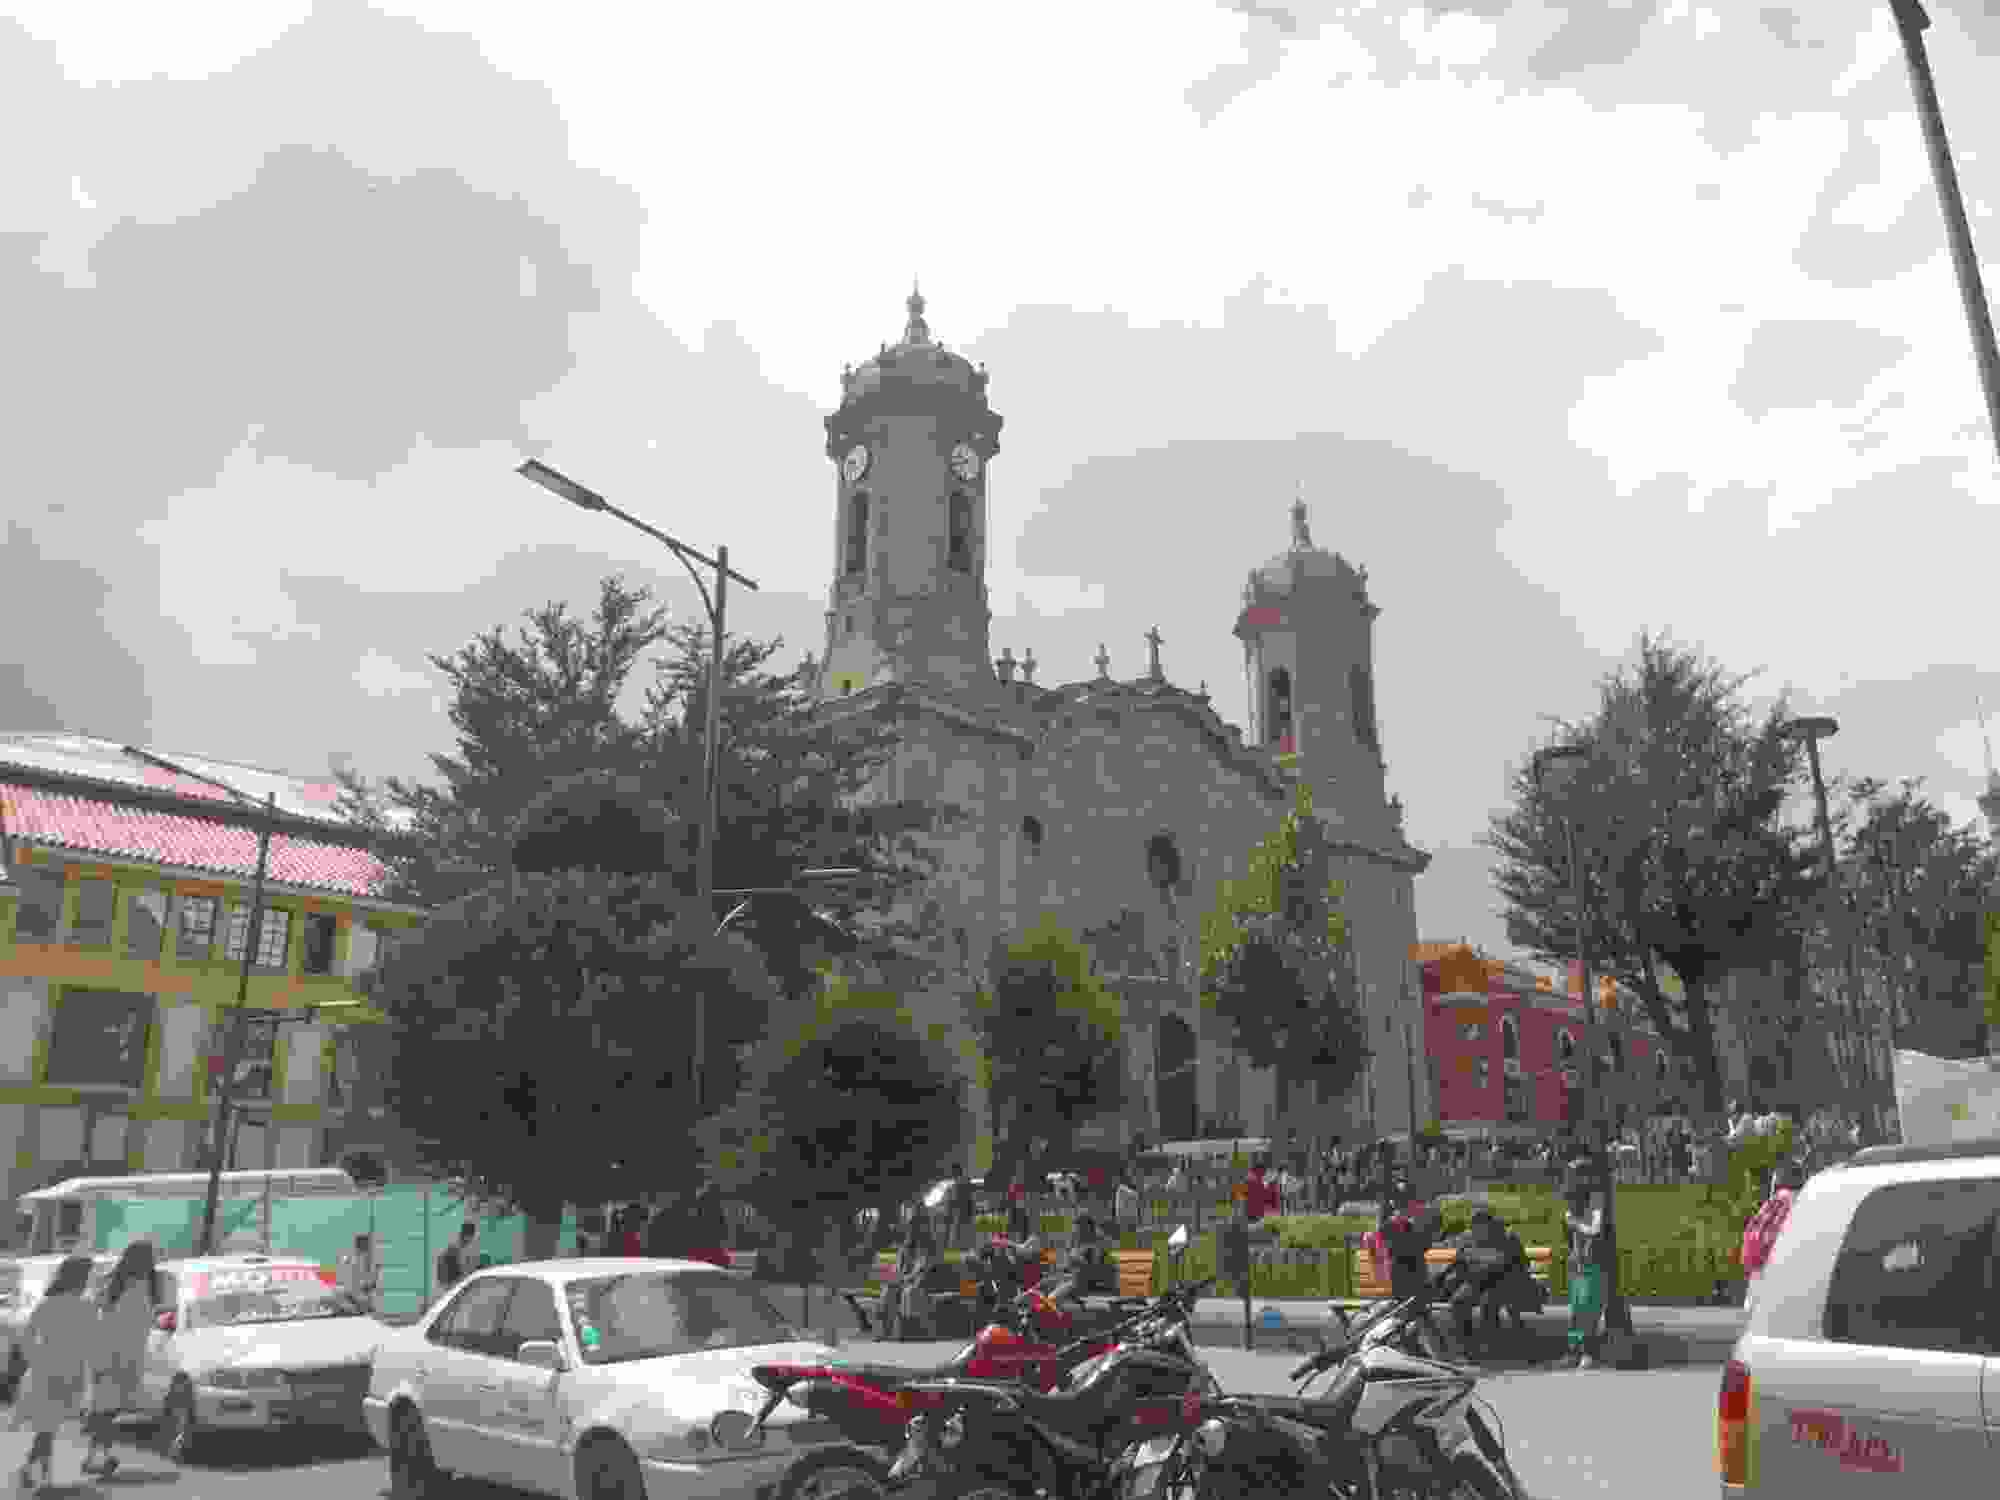
\includegraphics[width=\mywidth]{../wp-content/uploads/2015/04/wpid-wp-1428891310502.jpg} } 
 \newline
 Une église \newline
 \newline
\centerline{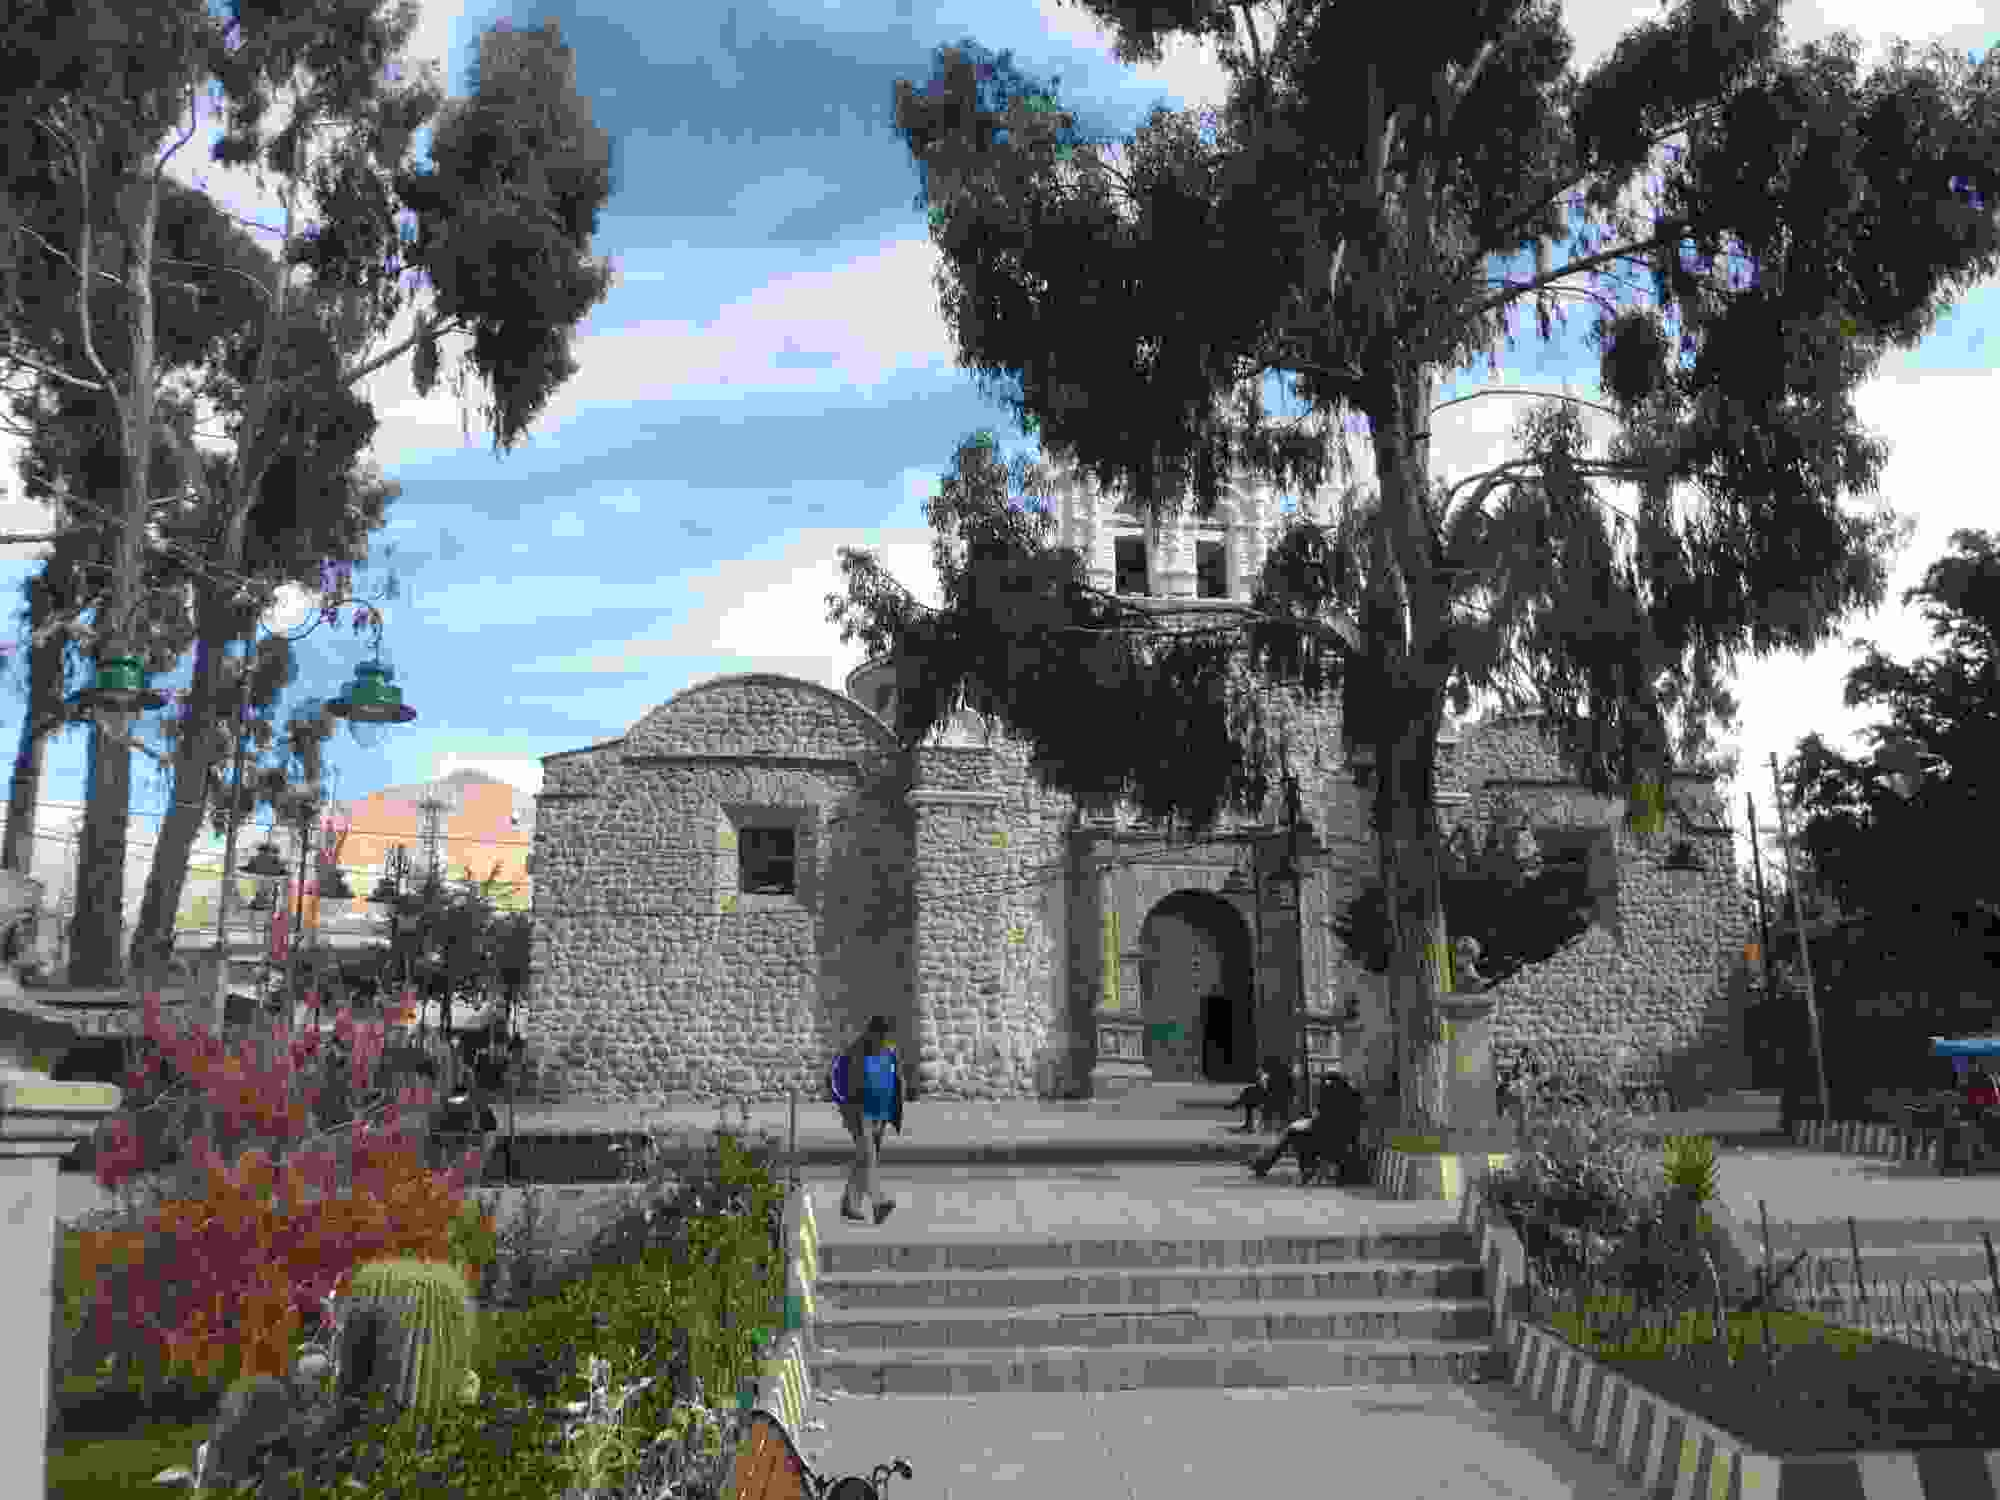
\includegraphics[width=\mywidth]{../wp-content/uploads/2015/04/wpid-wp-1428891346885.jpg} } 
 \newline
 Le couvent Santa Teresa, visite guidée intéressante sur la vie des soeurs à l'époque coloniale : une fois entrées à l'âge de 15 ans celles ci étaient cloîtrées le reste de leur vie sans aucun contact avec l'extérieur.  \newline
 \newline
\centerline{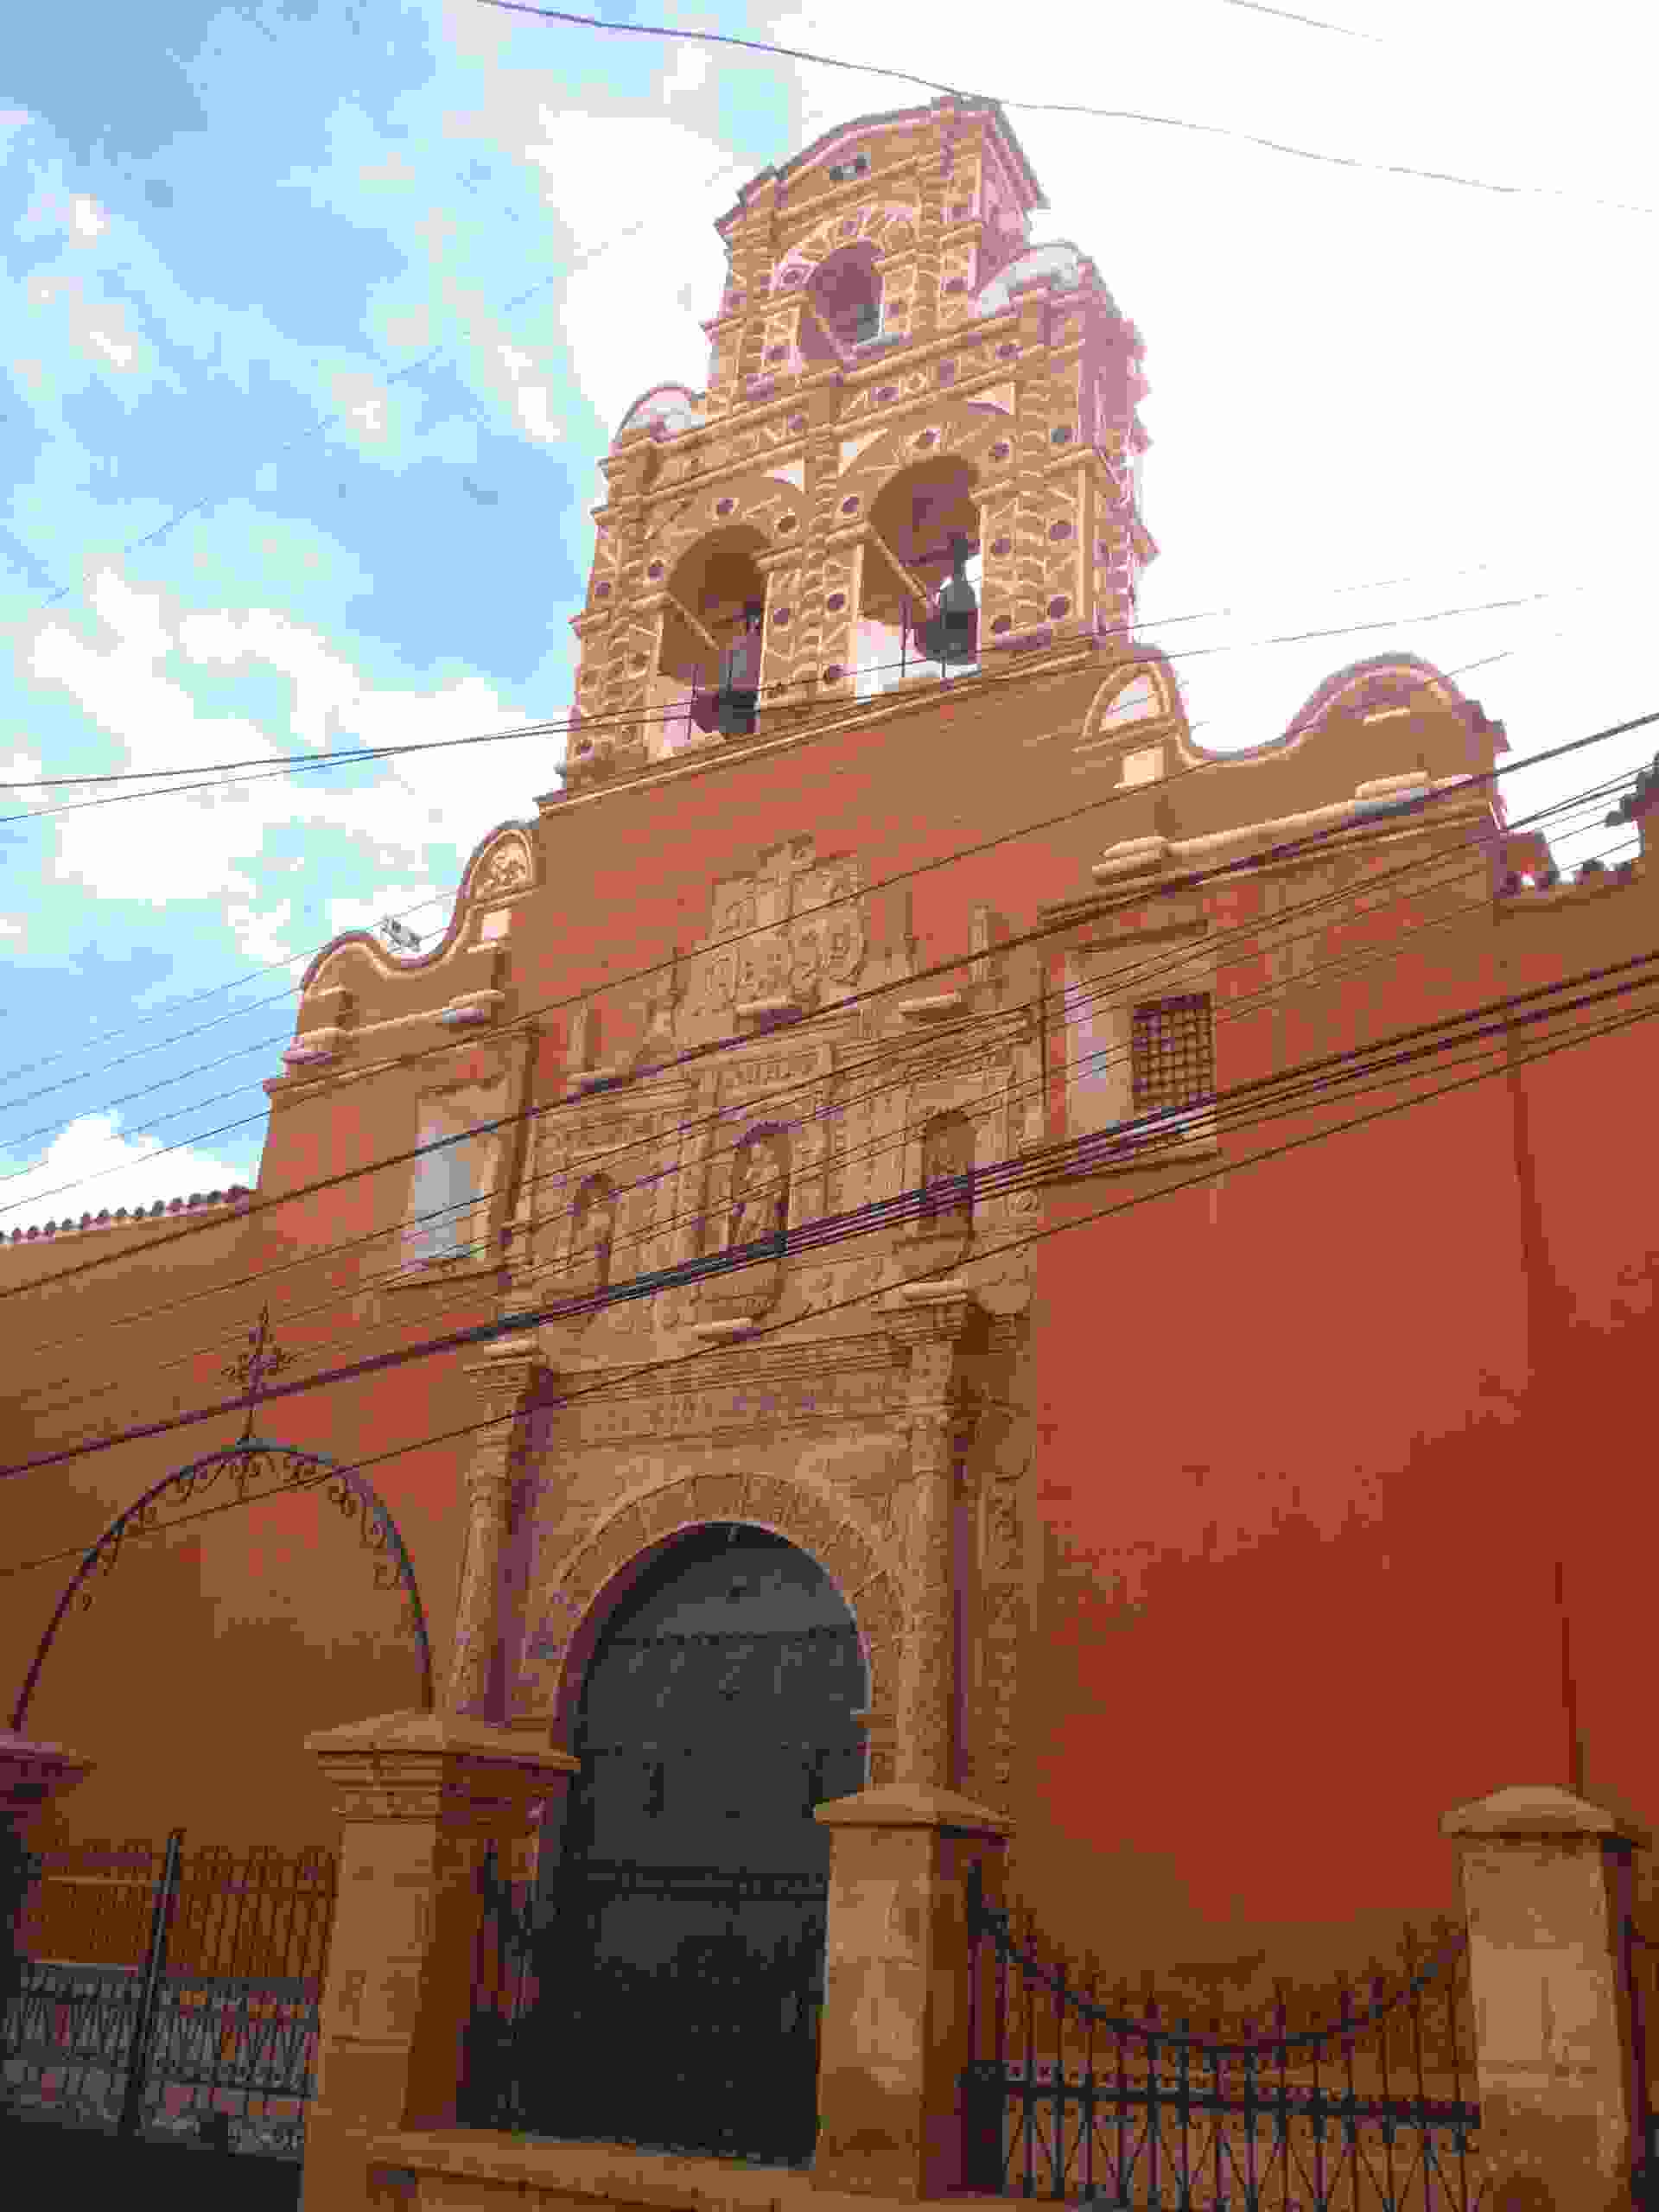
\includegraphics[width=\mywidth]{../wp-content/uploads/2015/04/wpid-wp-1428891737578.jpg} } 
 \newline
 La Casa de la Moneda.  \newline
 \newline
\centerline{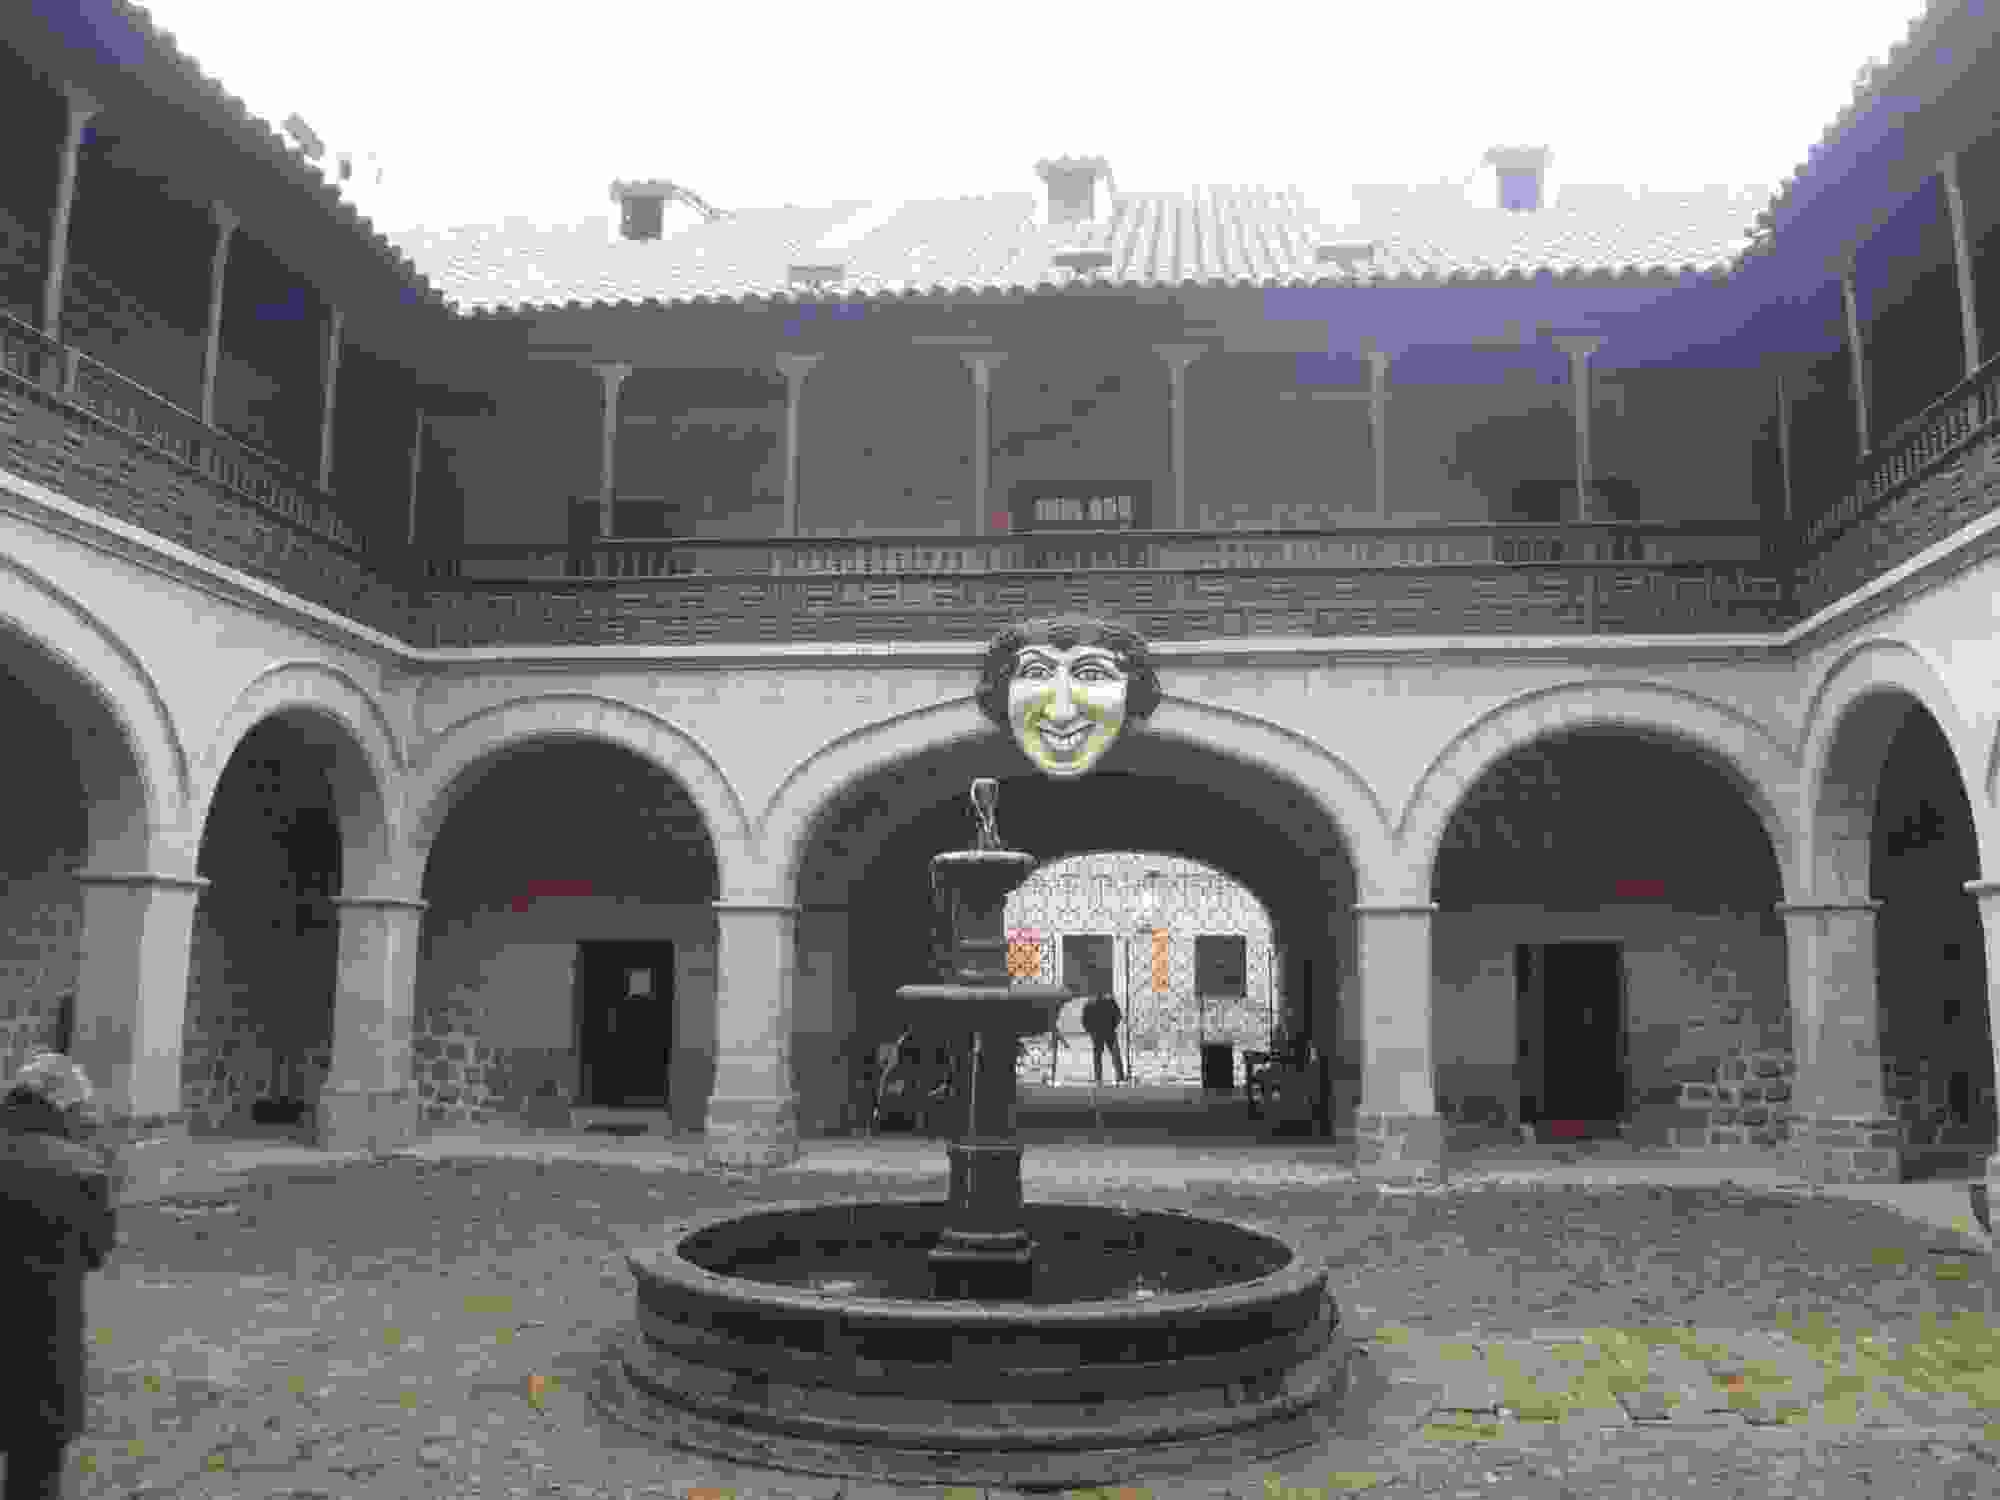
\includegraphics[width=\mywidth]{../wp-content/uploads/2015/04/wpid-wp-1428891875565.jpg} } 
 \newline
 Mais Potosi ce sont avant tout les mines d'argent, creusées dans le Cerro Rico. \newline
 \newline
\centerline{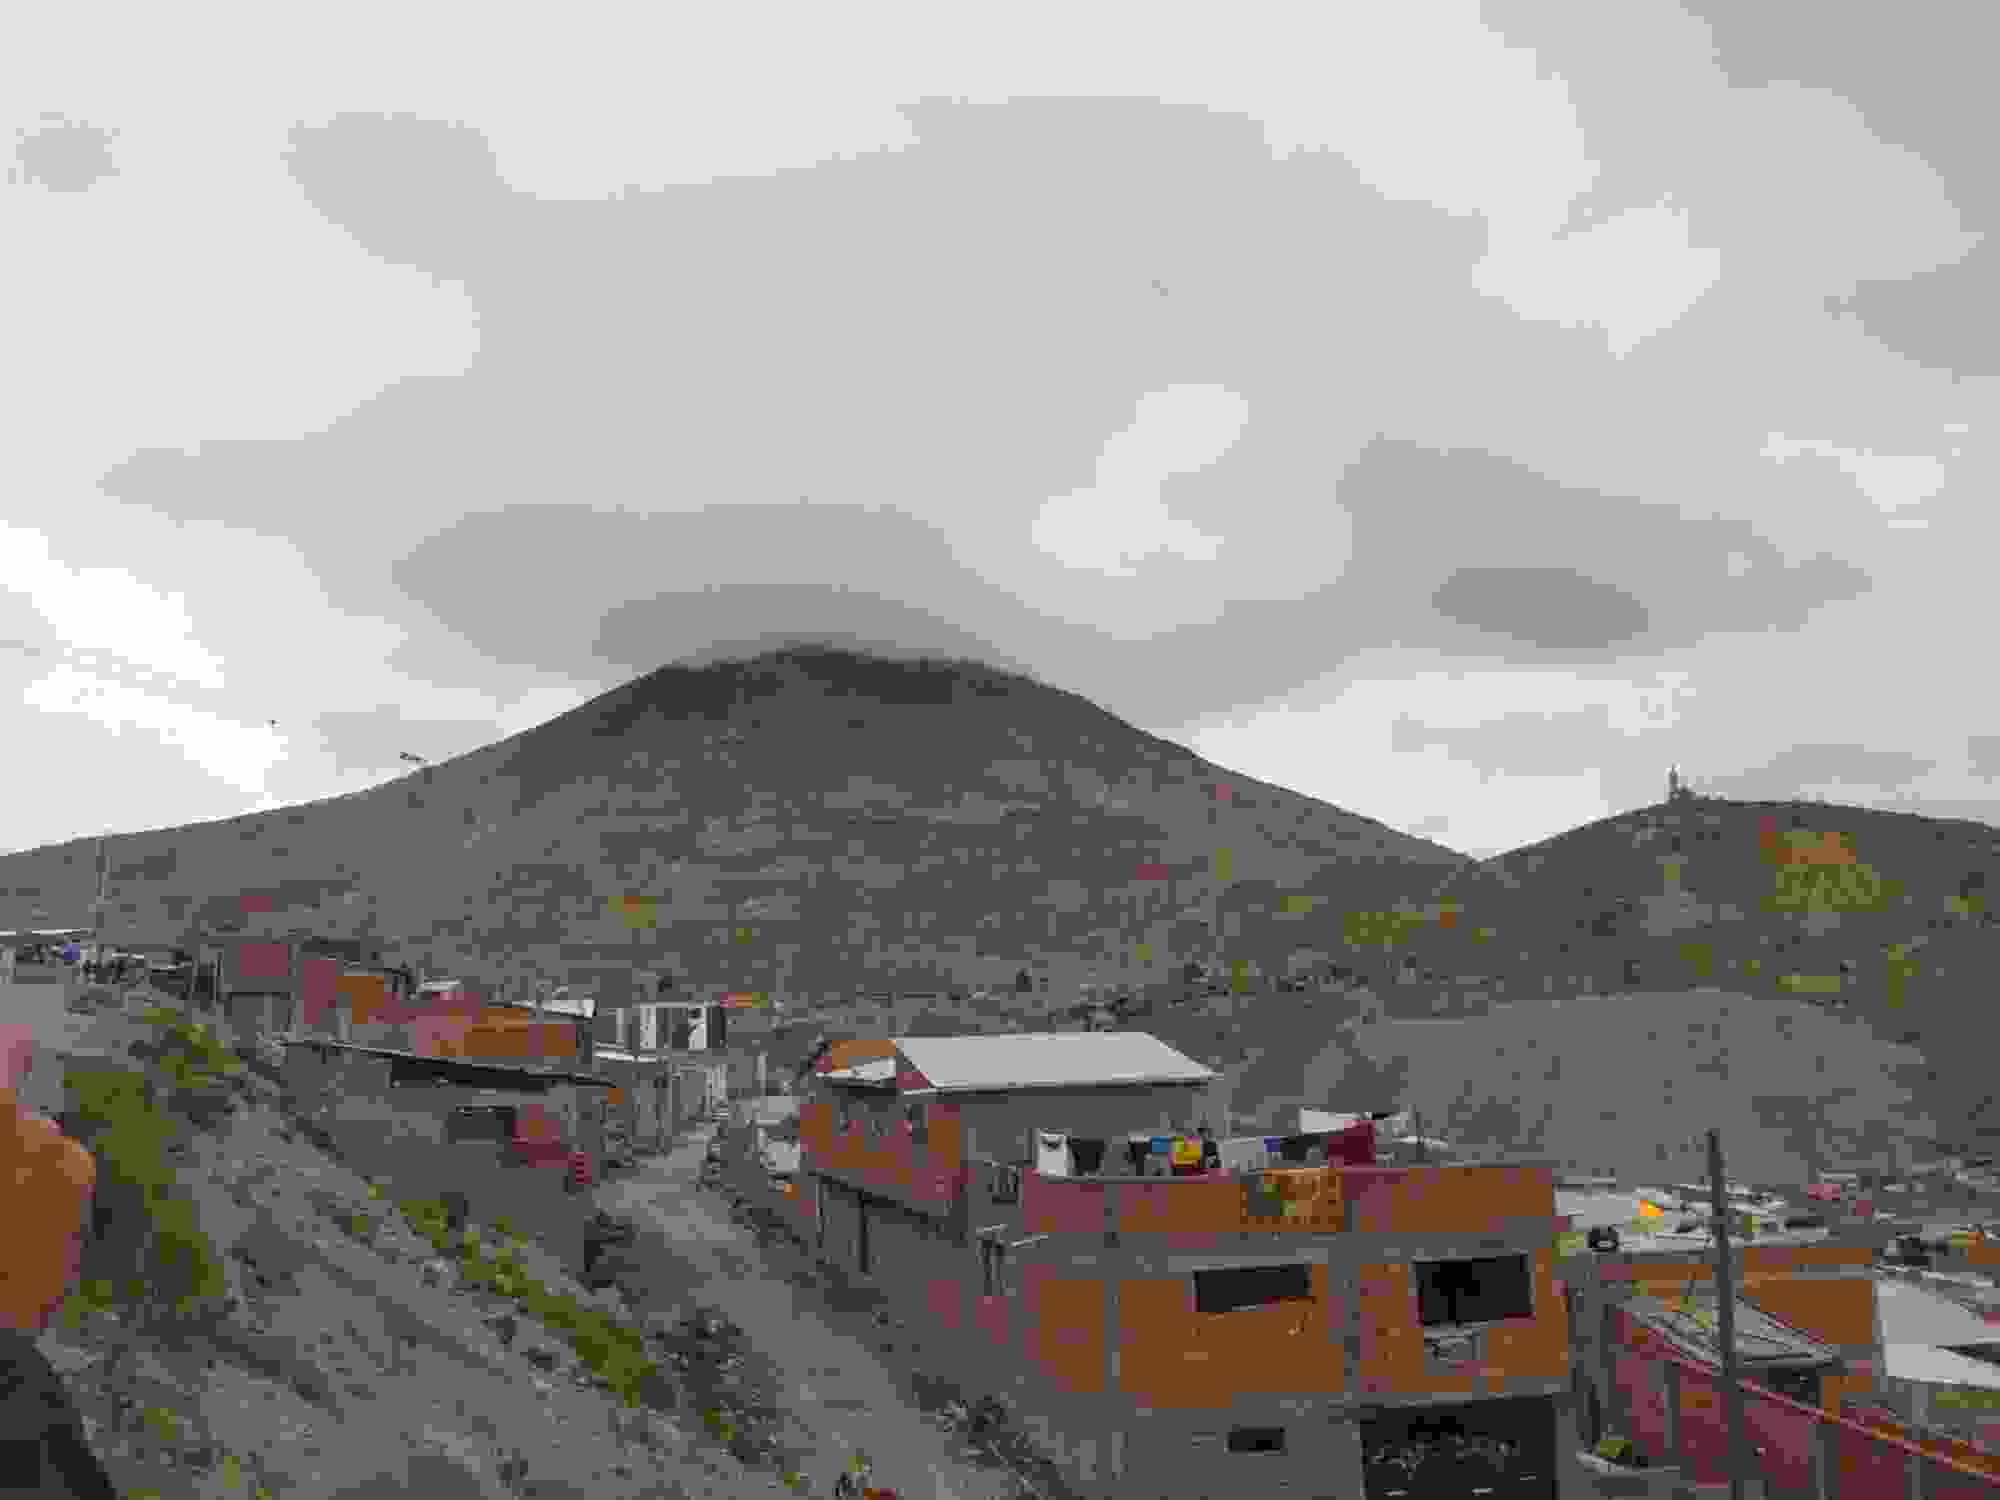
\includegraphics[width=\mywidth]{../wp-content/uploads/2015/04/wpid-wp-1428891958963.jpg} } 
 \newline
 La visite commence au marché des mineurs pour acheter des cadeaux pour les mineurs : feuilles de coca, boissons. \newline
 \newline
\centerline{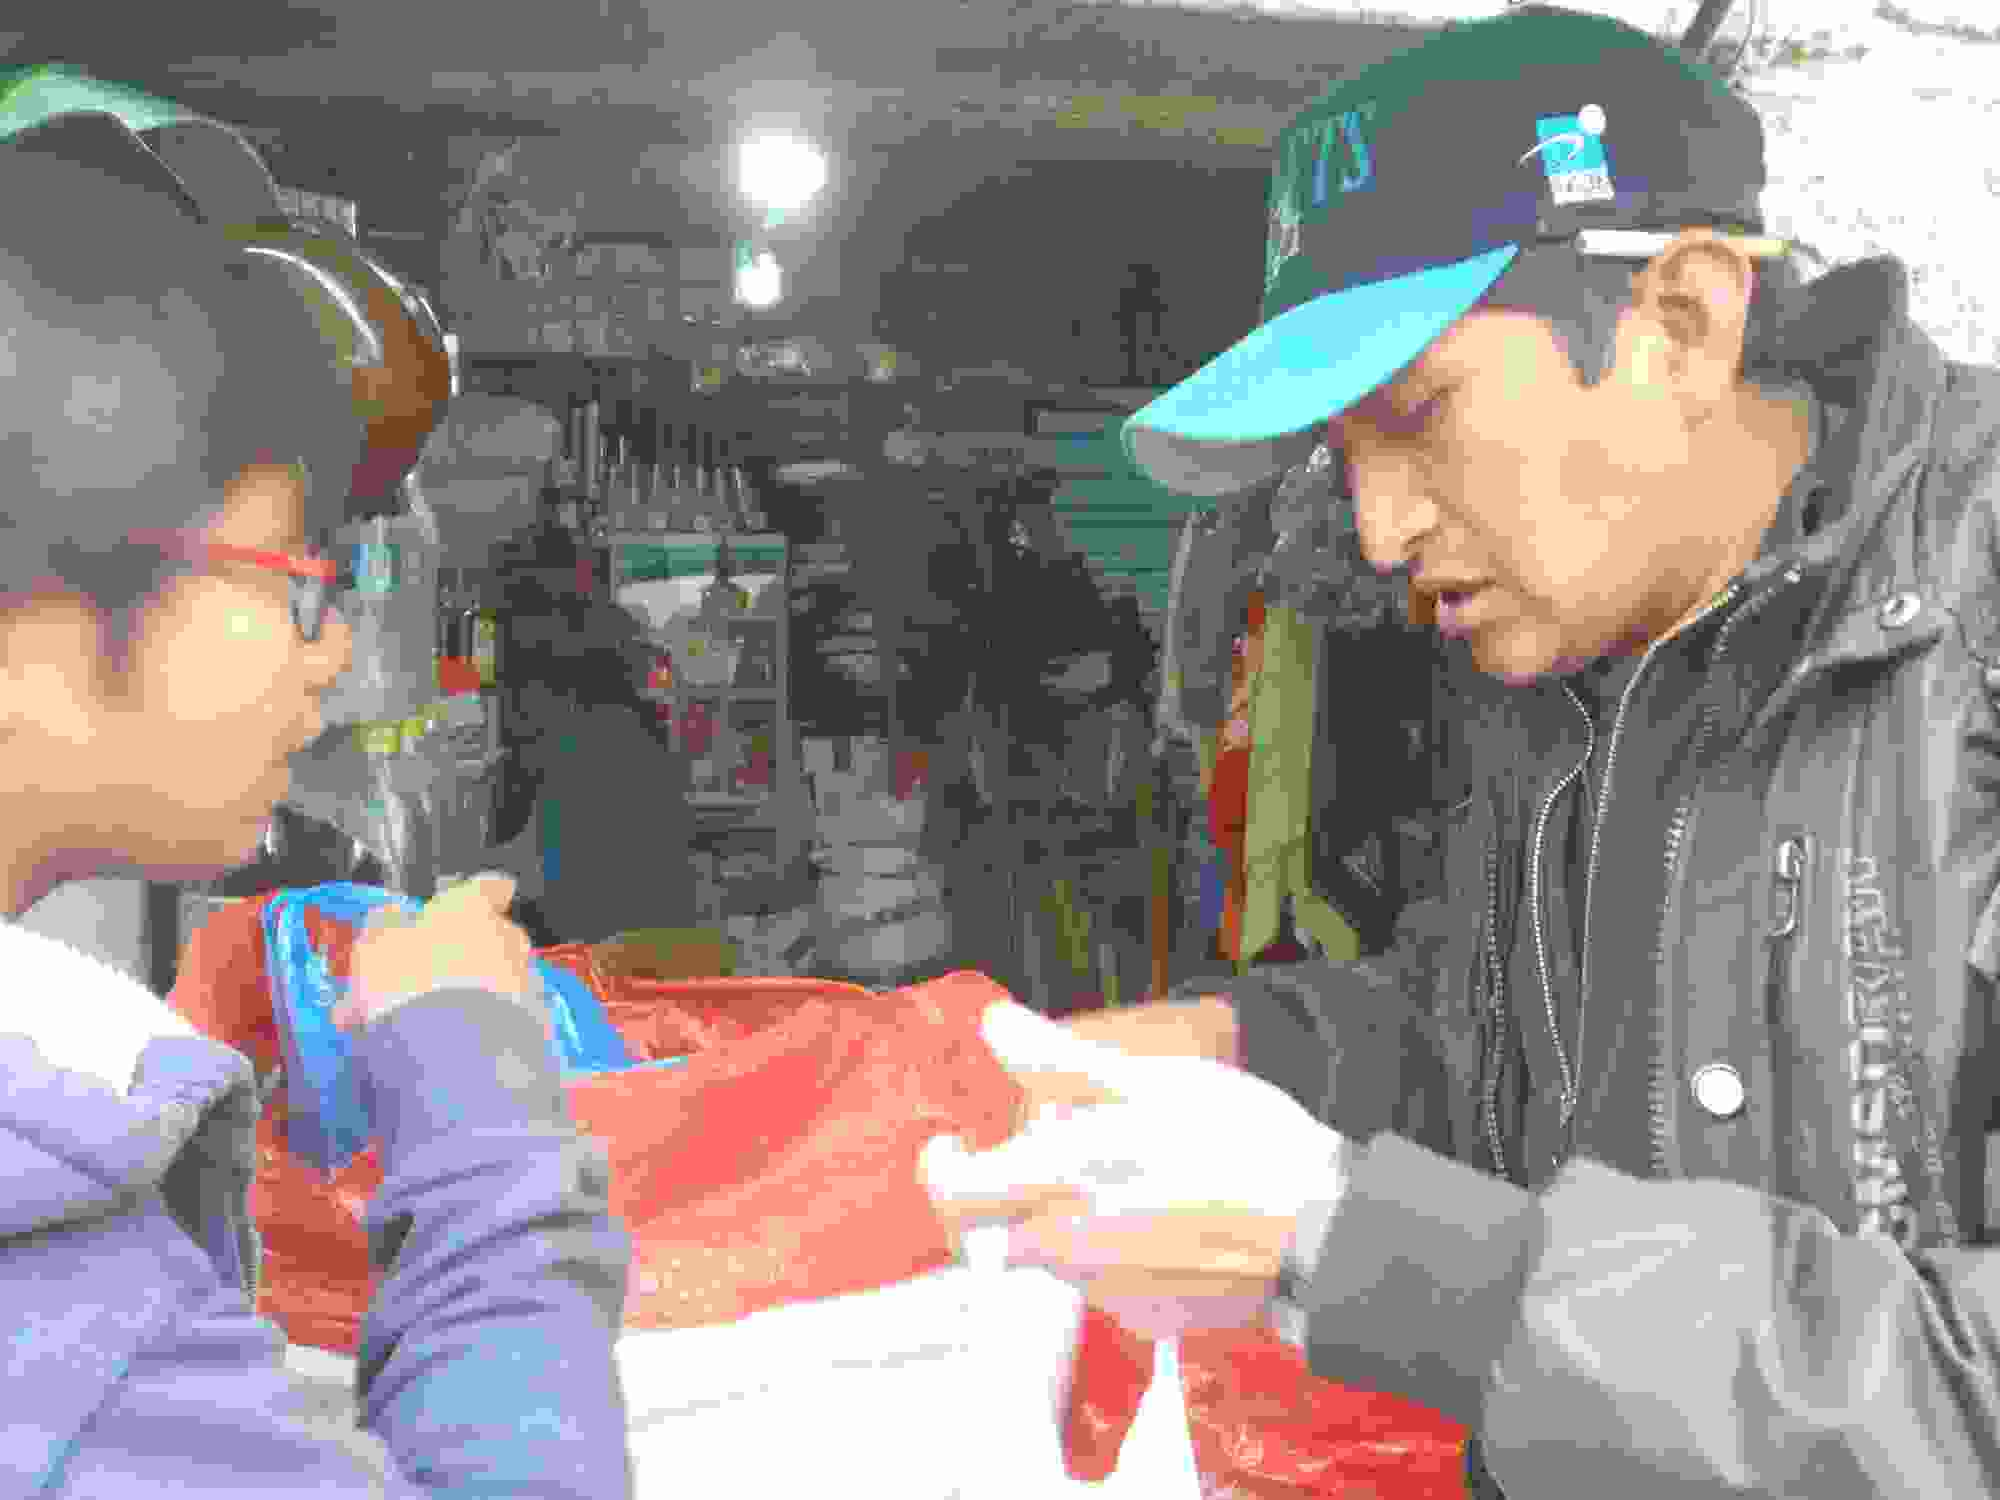
\includegraphics[width=\mywidth]{../wp-content/uploads/2015/04/wpid-wp-1428892276575.jpg} } 
 \newline
 On enfile la tenue de protection.  \newline
 \newline
\centerline{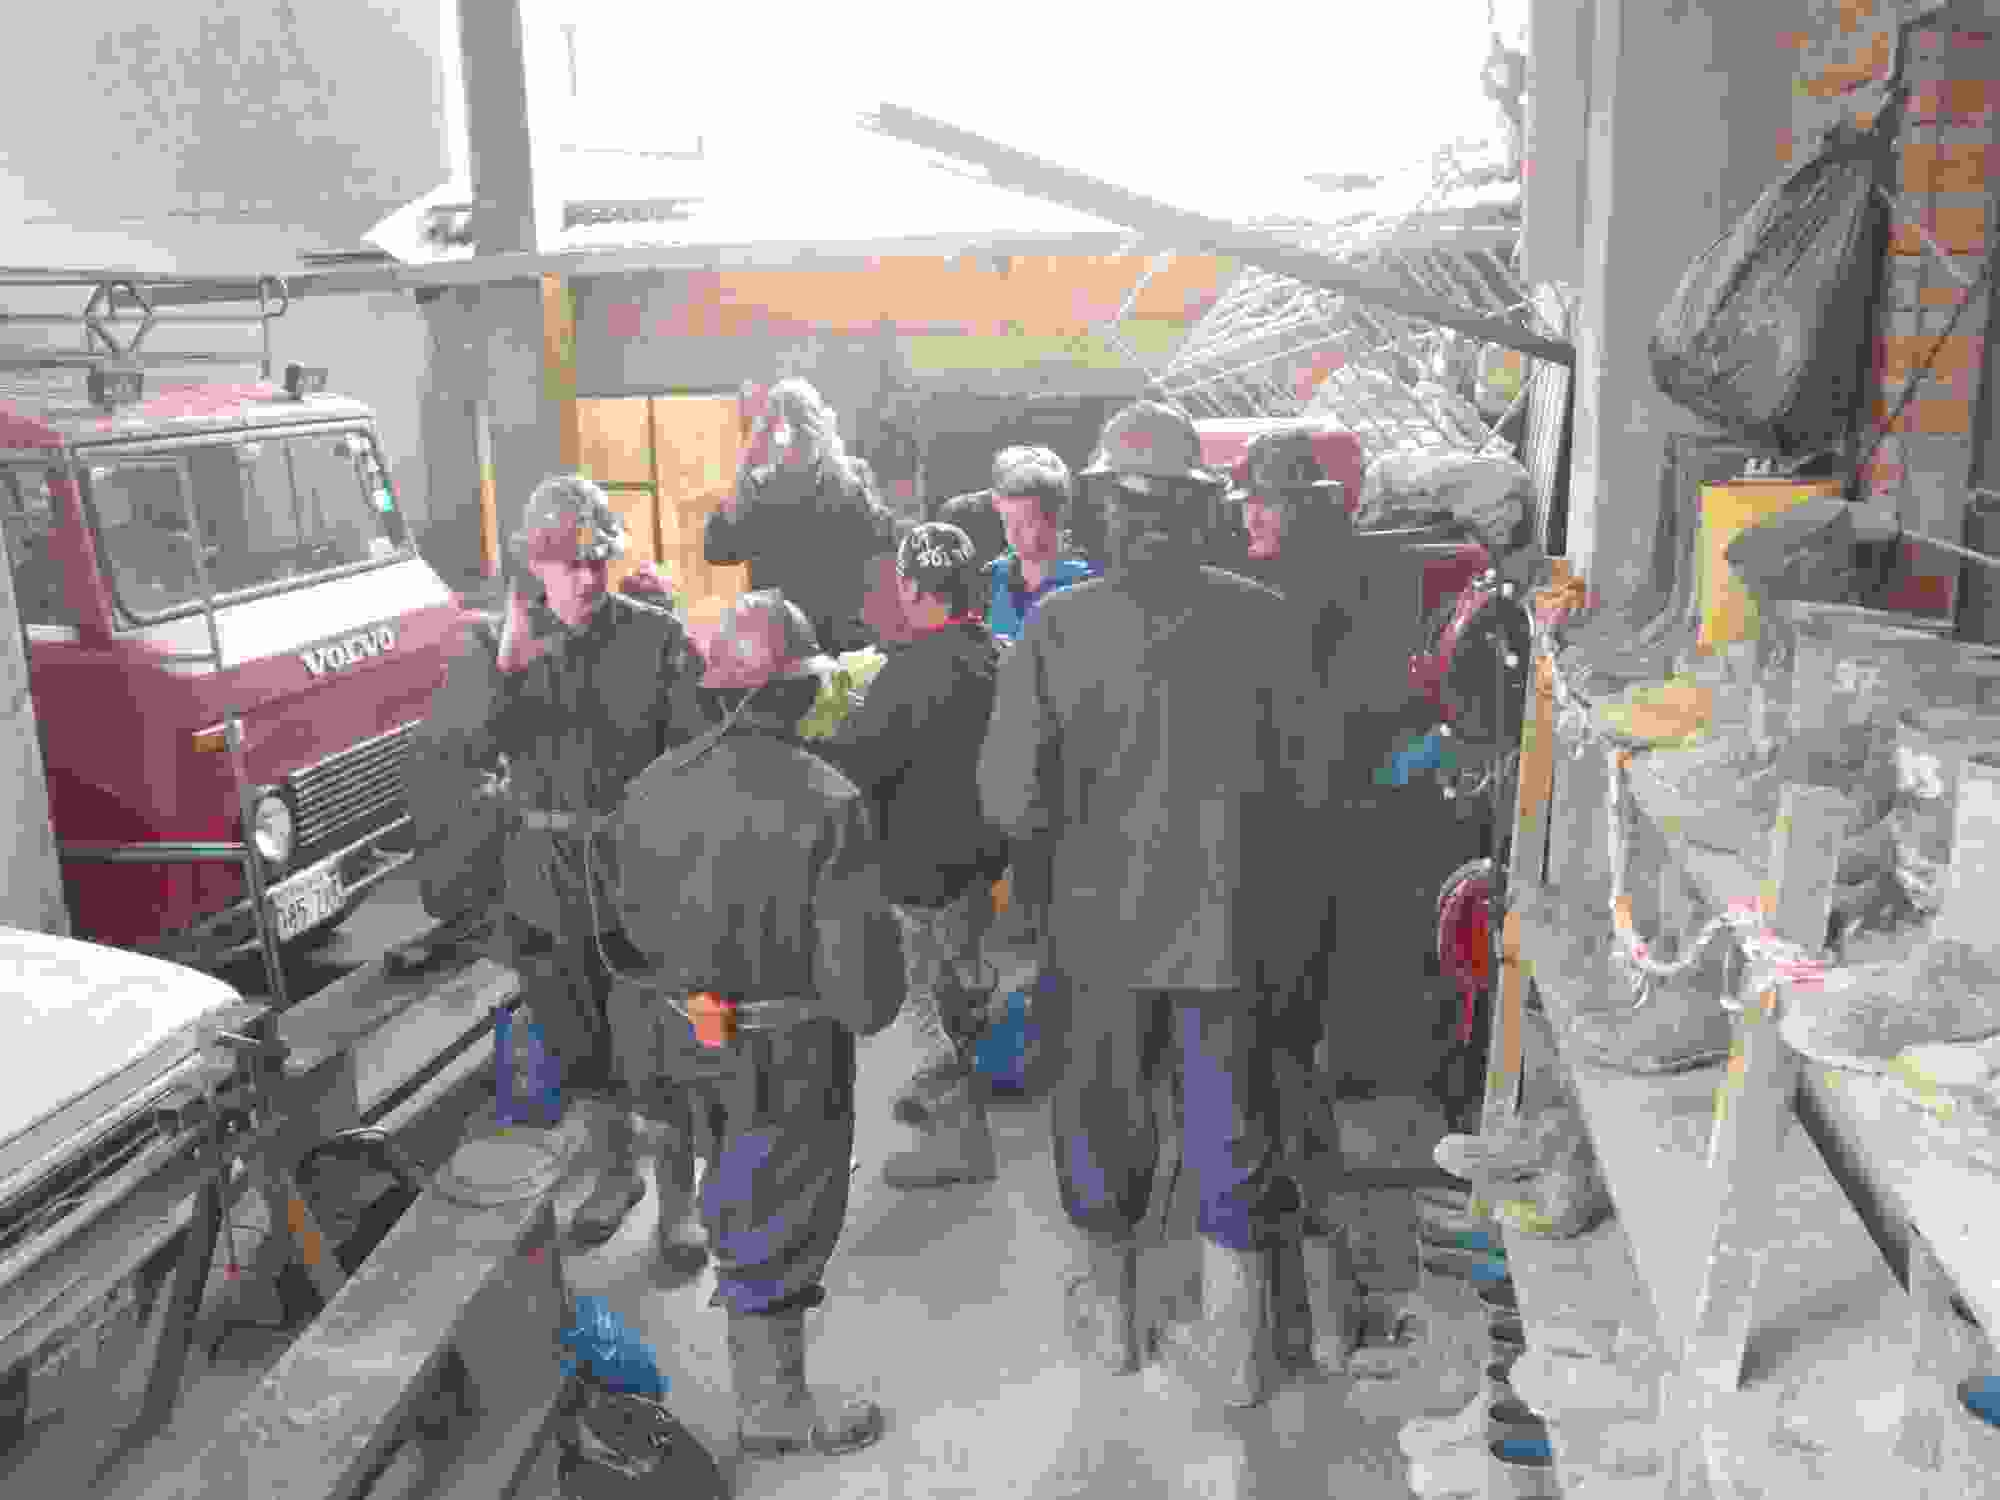
\includegraphics[width=\mywidth]{../wp-content/uploads/2015/04/wpid-wp-1428892402383.jpg} } 
 \newline
 Visite d'une usine de traitement des minerais : argent, zinc et plomb sont extraits ici.  \newline
 \newline
\centerline{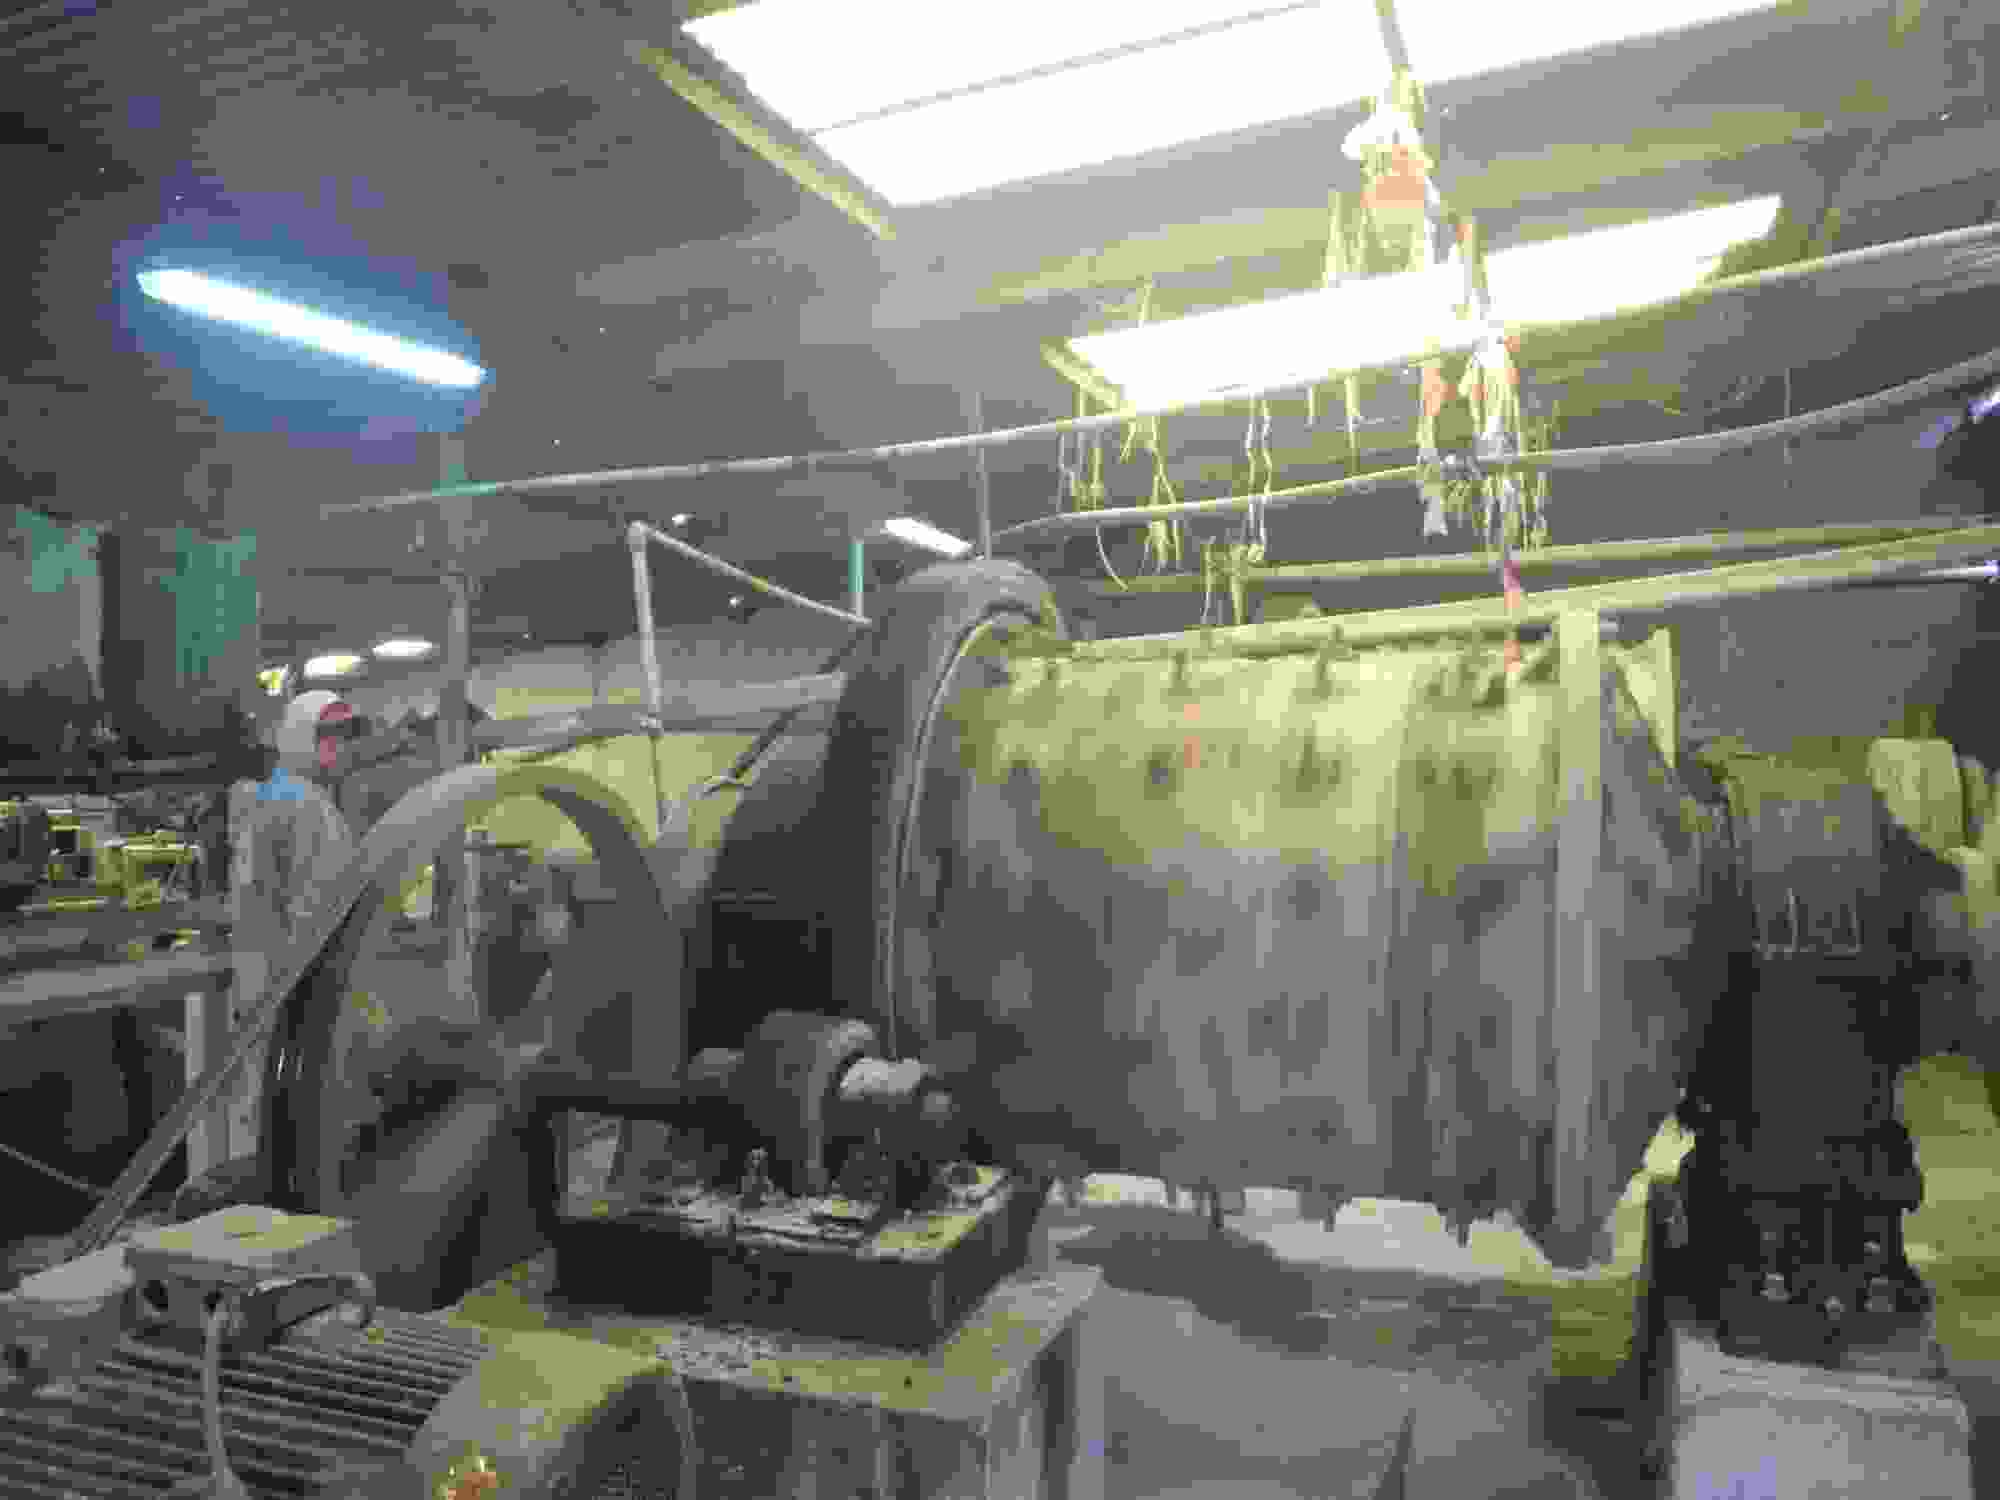
\includegraphics[width=\mywidth]{../wp-content/uploads/2015/04/wpid-wp-1428892501544.jpg} } 
 \newline
 \newline
\centerline{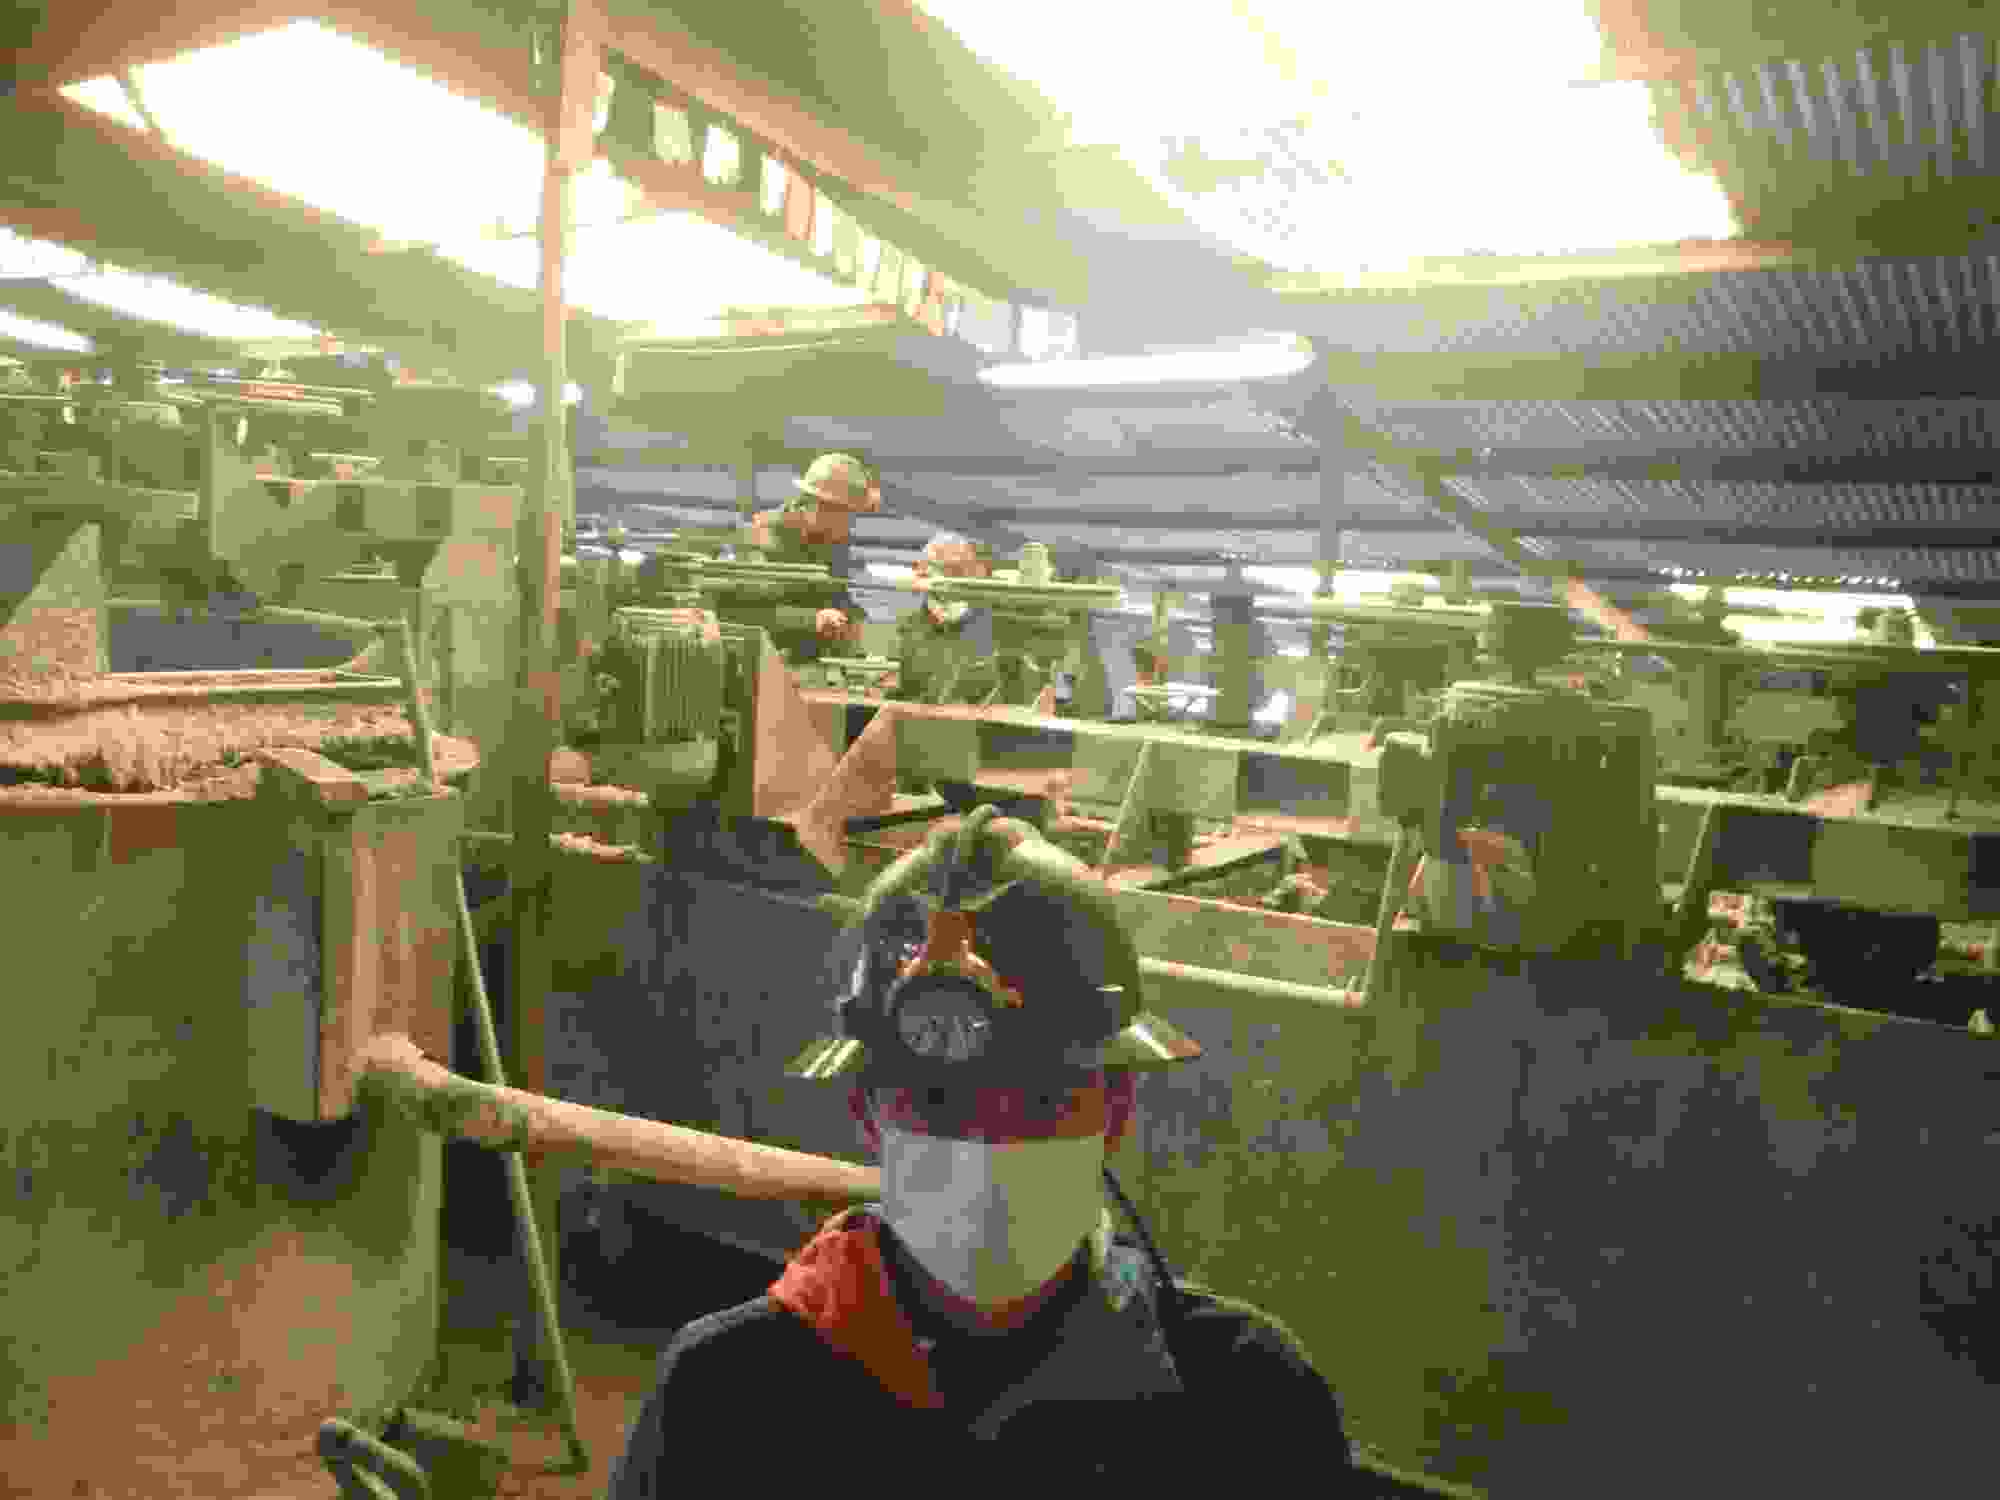
\includegraphics[width=\mywidth]{../wp-content/uploads/2015/04/wpid-wp-1428892515847.jpg} } 
 \newline
 Puis c'est la visite de la mine, guidée par un ancien mineur.  \newline
 \newline
\centerline{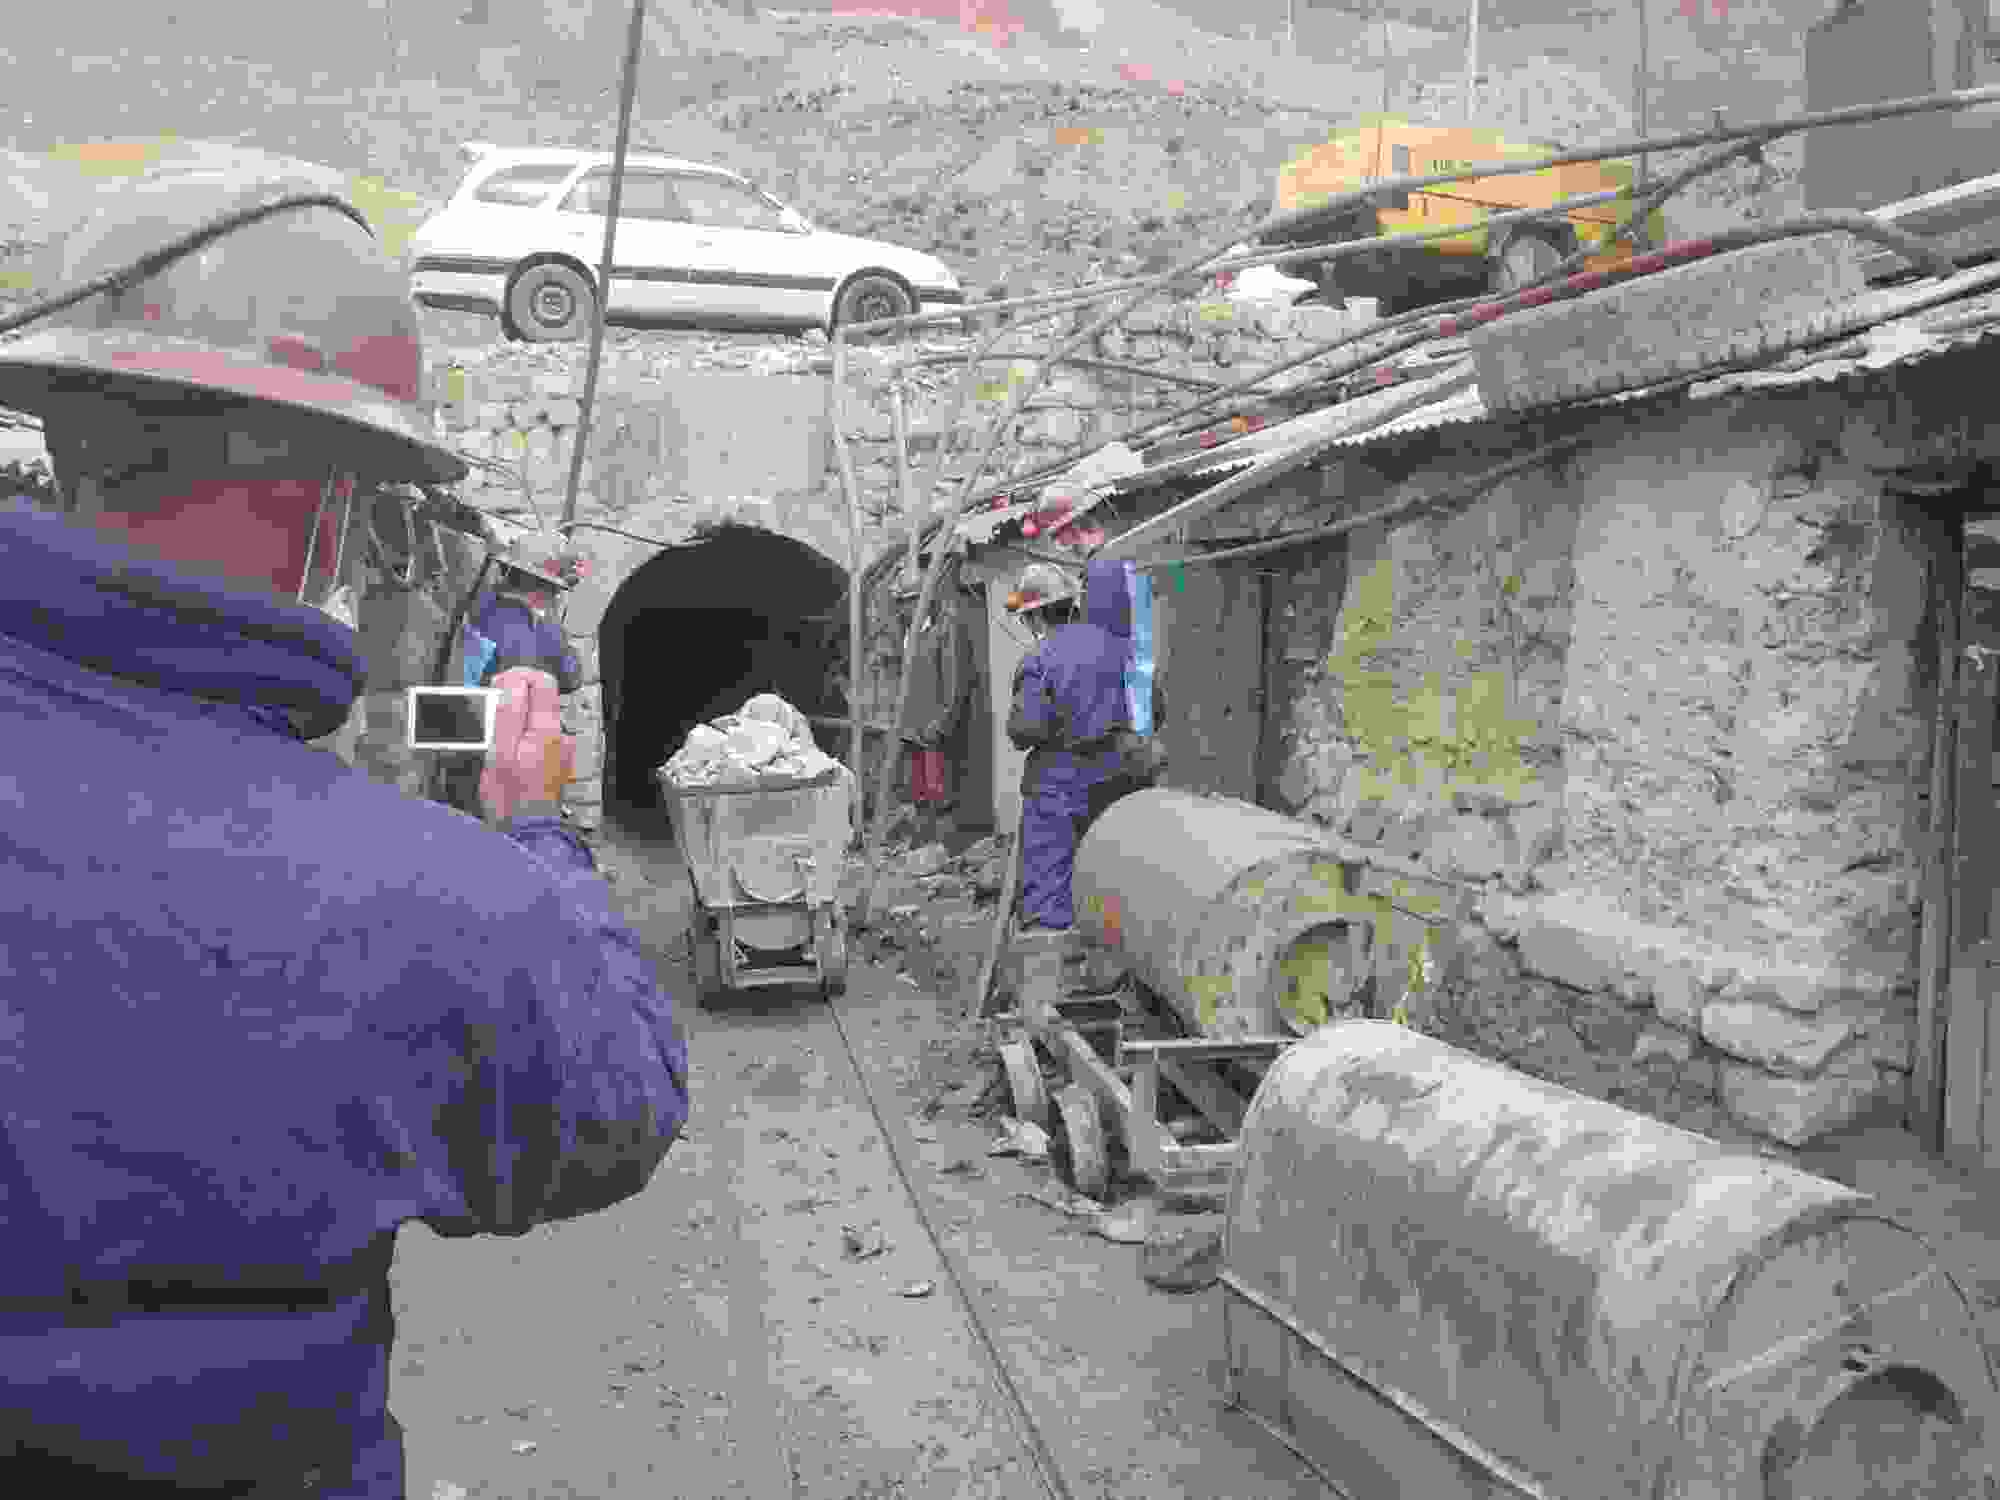
\includegraphics[width=\mywidth]{../wp-content/uploads/2015/04/wpid-wp-1428892613443.jpg} } 
 \newline
 «El Tio» porte bonheur pour les mineurs.  \newline
 \newline
\centerline{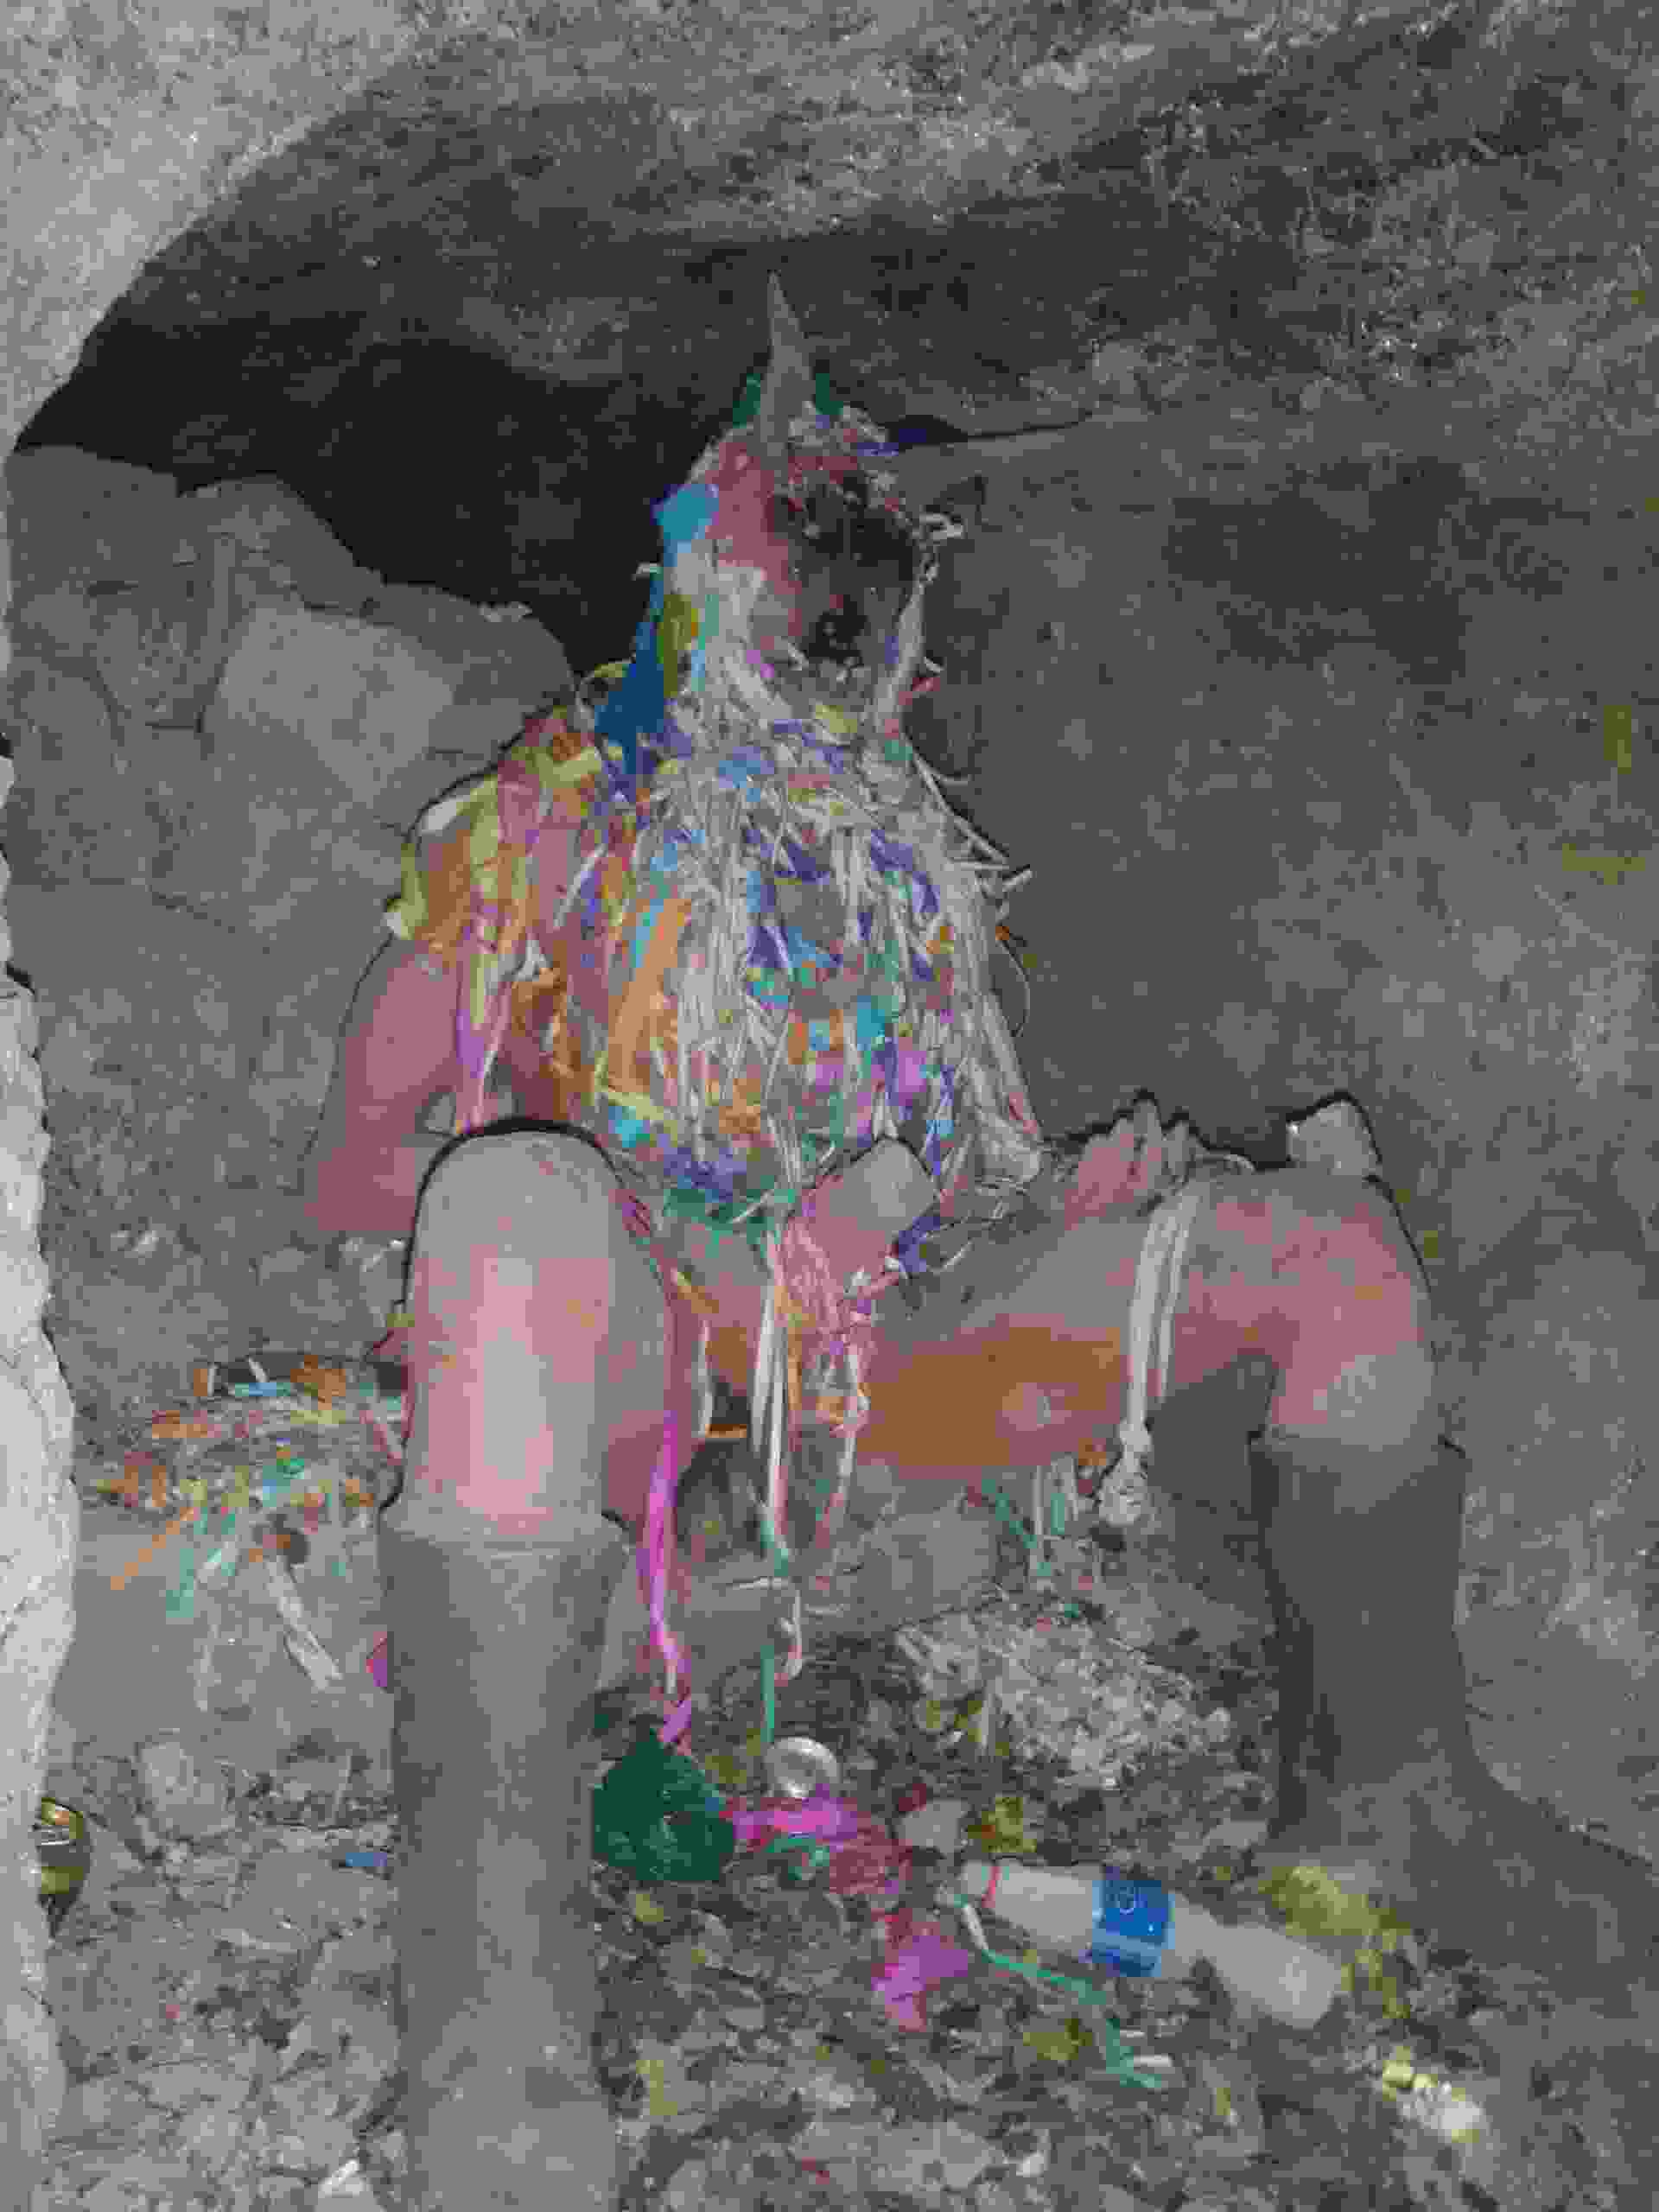
\includegraphics[width=\mywidth]{../wp-content/uploads/2015/04/wpid-wp-1428892725739.jpg} } 
 \newline
 Les galeries, on doit marcher courbé et la plupart du temps dans la boue.  \newline
 \newline
\centerline{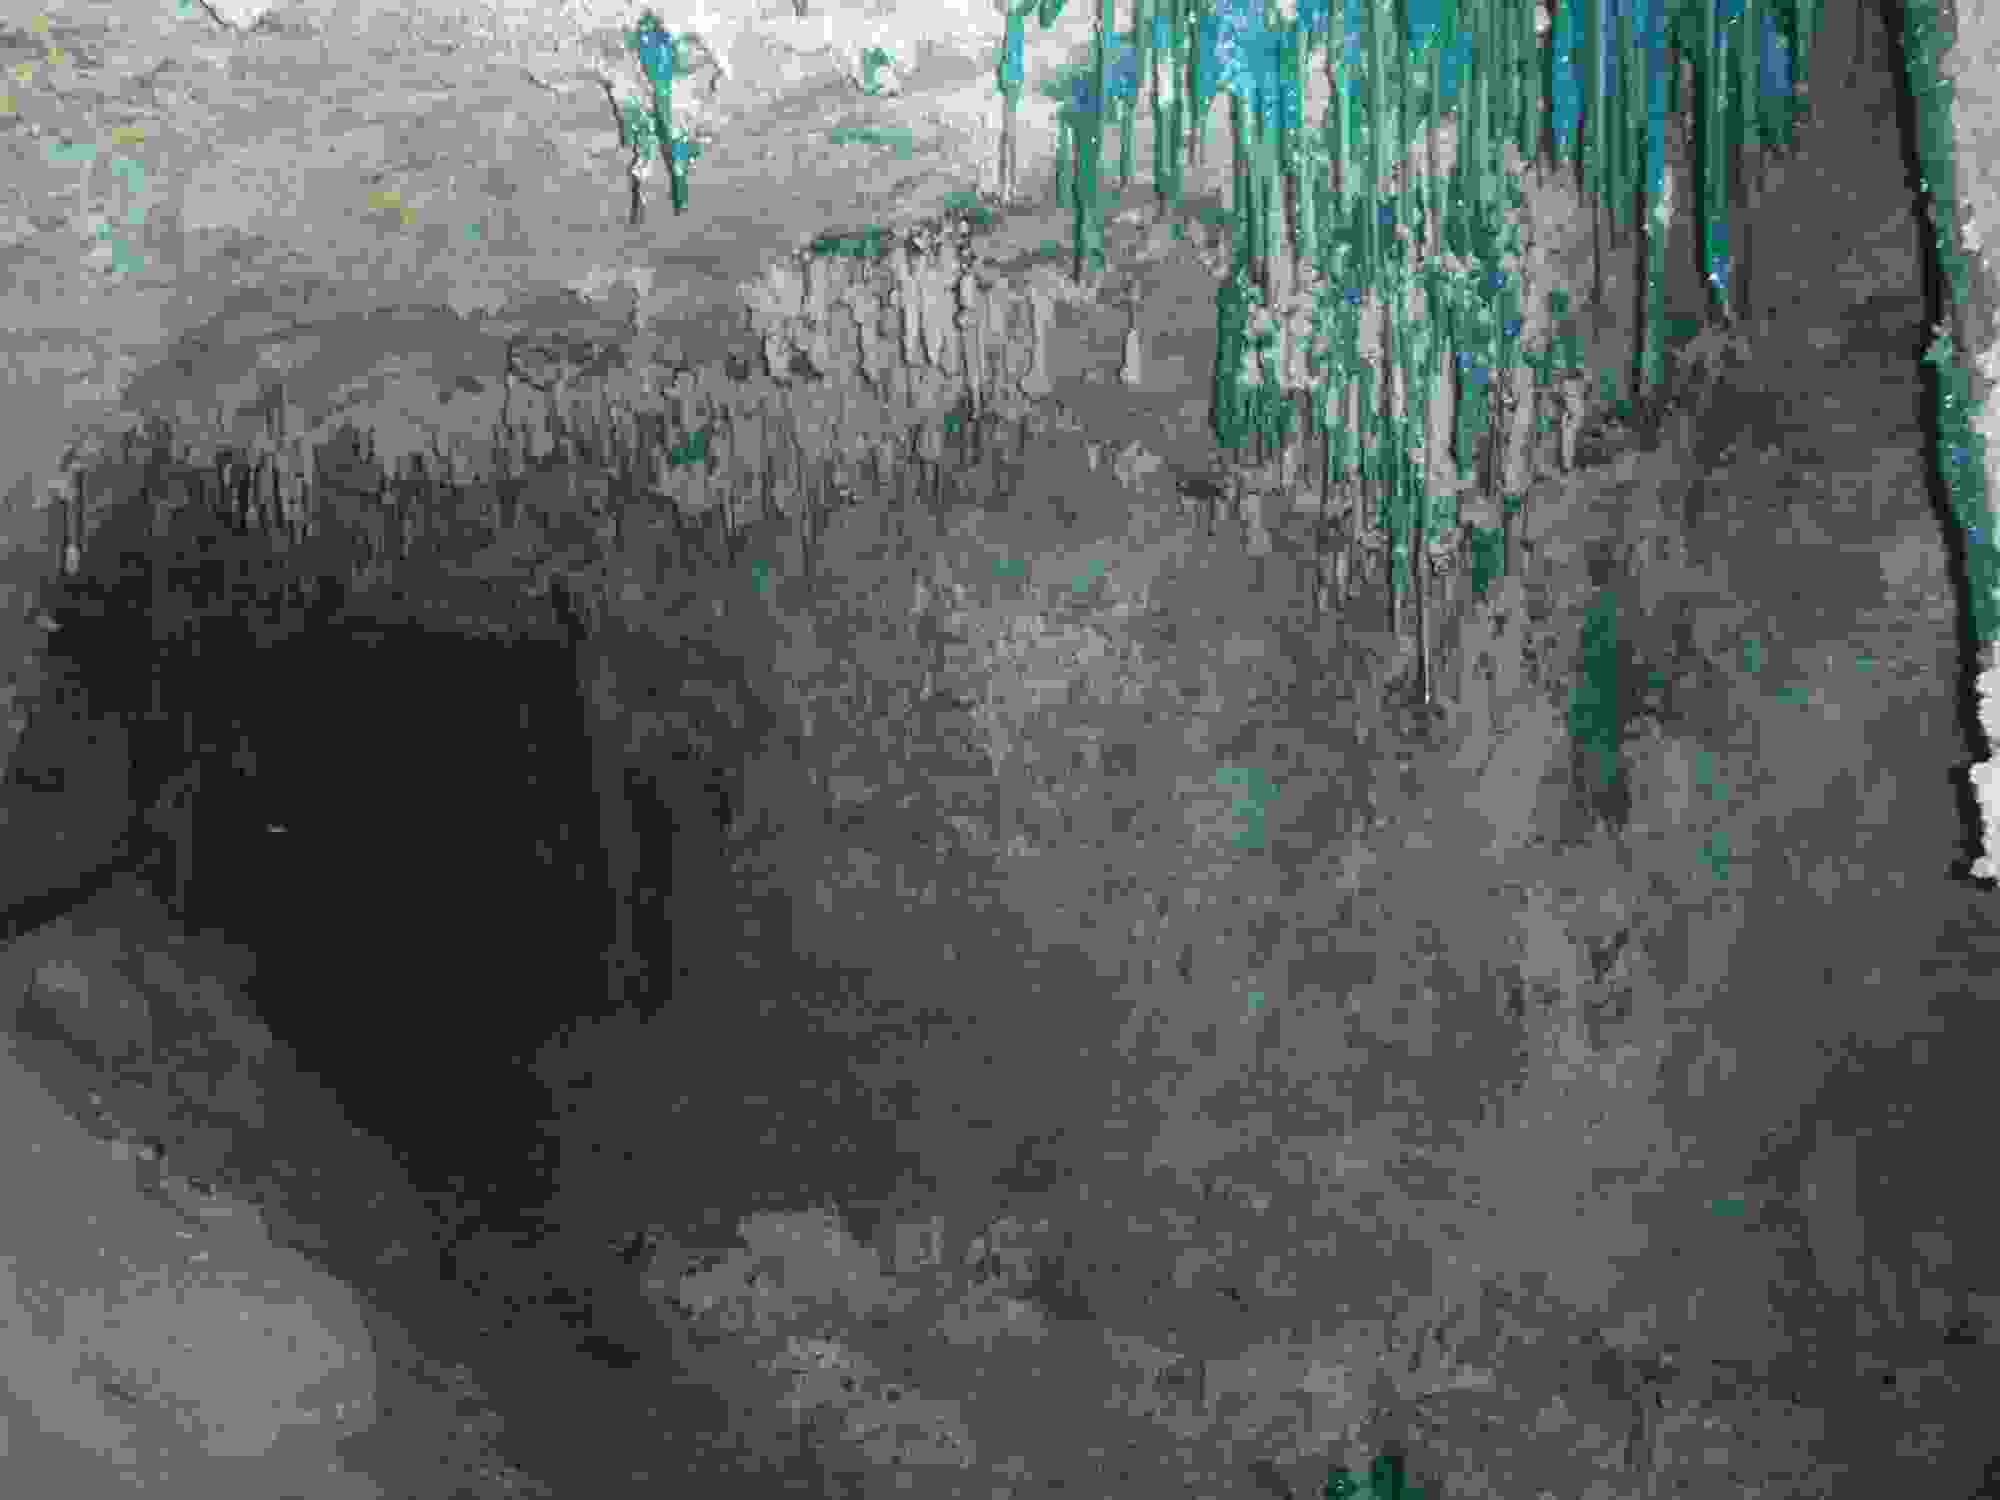
\includegraphics[width=\mywidth]{../wp-content/uploads/2015/04/wpid-wp-1428892808307.jpg} } 
 \newline
 On croise quelques mineurs : les feuilles de coca leur donnent l'énergie pour travailler toute la journée sans manger. \newline
 Ce travail usant et dangereux leur permet de gagner 2 à 3 fois le salaire minimum bolivien.  \newline
 \newline
\centerline{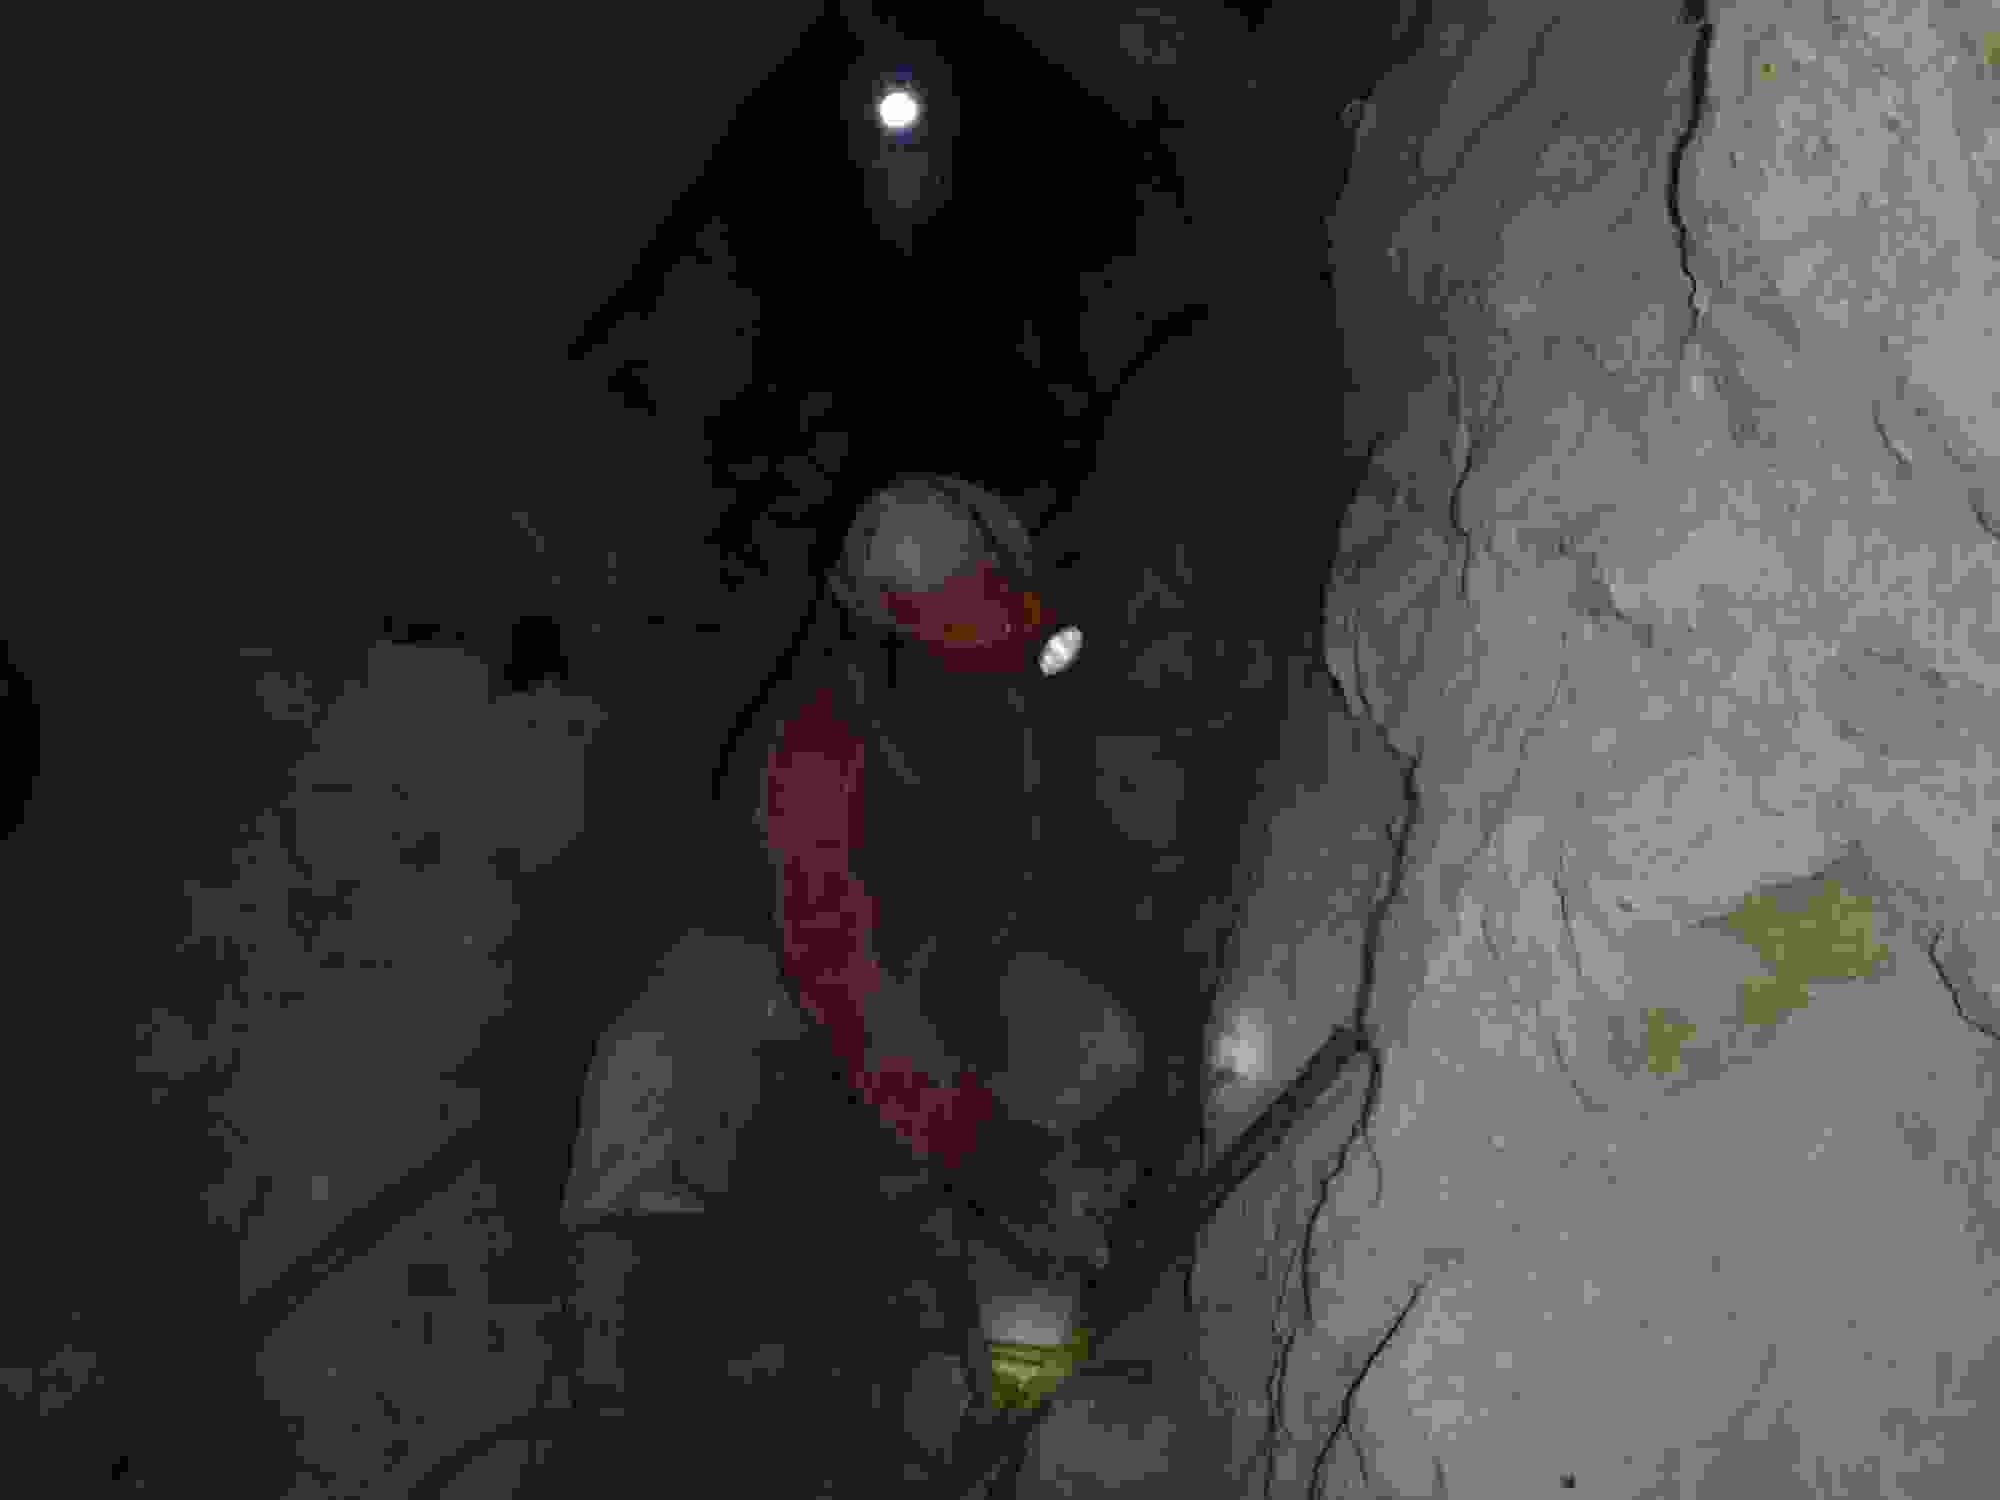
\includegraphics[width=\mywidth]{../wp-content/uploads/2015/04/wpid-wp-1428892913145.jpg} } 
 \newline
 \newline
\centerline{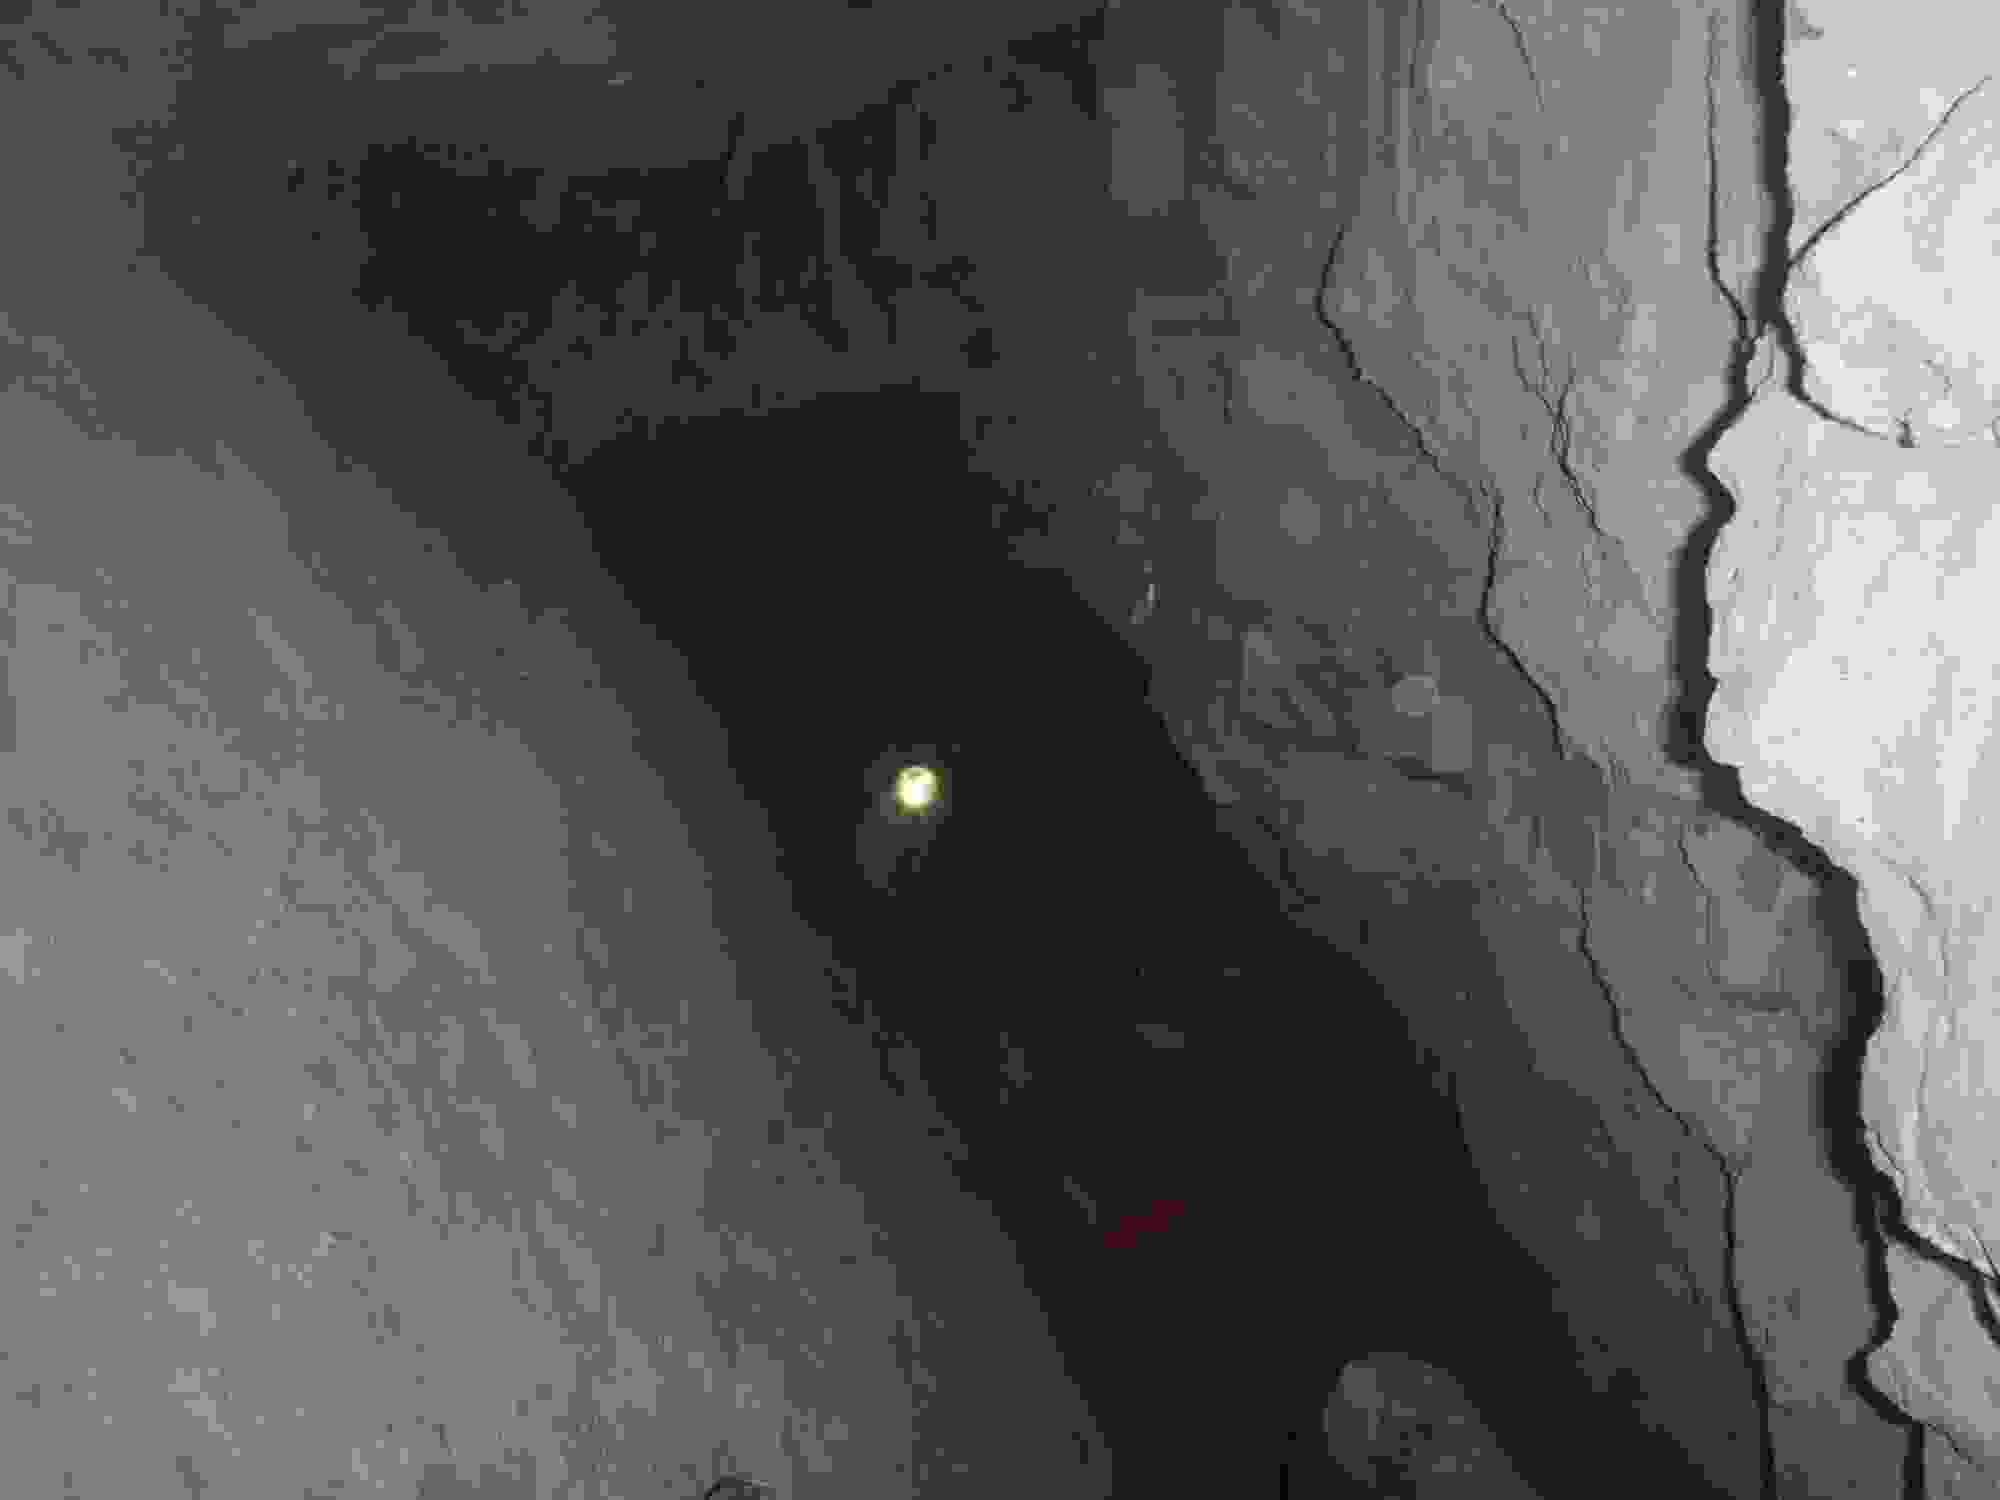
\includegraphics[width=\mywidth]{../wp-content/uploads/2015/04/wpid-wp-1428892926957.jpg} } 
 \newline

\newpage
 
